%%%%%%%%%%%%%%%%%%%%%%%%%%%%%%%%%%%%%%%%%%%%%%
%
%		My Thesis
%
%		EDOC Template
%		2011
%
%%%%%%%%%%%%%%%%%%%%%%%%%%%%%%%%%%%%%%%%%%%%%%

% IMPORTANT: To change the color of the rectangles, go to head/settings_epfl_template.tex, line 36, color bluegray

\documentclass[a4paper,11pt]{DoctoralThesis}
\input{head/settings_epfl_template.tex} % epfl template packages are here
%%%%%%%%%%%%%%%%%%%%%%%%%%%%%%%%%%%%%%%%%%%%%%
%
%		Thesis Settings
%		Custom settings
%
%		2011
%
%%%%%%%%%%%%%%%%%%%%%%%%%%%%%%%%%%%%%%%%%%%%%%

% %
% %   Use this file for your own custom packages, command-definitions, etc...
% %
% % 

\usepackage[utf8]{inputenc} % Required for inputting international characters
\usepackage[T1]{fontenc} % Output font encoding for international characters
\DeclareMathAlphabet{\mathcal}{OMS}{cmsy}{m}{n} % because fourrier font makes \mathcal too fancy
\usepackage{xfrac}
\usepackage[section]{placeins}
%\usepackage{mathpazo} % Use the Palatino font by default
%\usepackage{libertine}
%\usepackage{libertinust1math}
\usepackage[T1]{fontenc}
\usepackage{siunitx}
%\usepackage[backend=bibtex,style=ieee]{biblatex} % Use the bibtex backend with the authoryear citation style (which resembles APA)

% \usepackage[block=ragged,natbib=true]{biblatex}

%\usepackage{subcaption} % for subfigures
\usepackage{graphicx}
\usepackage{wrapfig}
%\usepackage{caption}
%\usepackage[caption=false]{subfig}
%\captionsetup[subfigure]{width=0.7\textwidth}
\graphicspath{{Figures/}{./}} % Specifies where to look for included images

\usepackage{tikz}
\usetikzlibrary{positioning,arrows,fit,backgrounds, patterns}

\usepackage[super]{nth}

%\usepackage[autostyle=true]{csquotes} % Required to generate language-dependent quotes in the bibliography

\usepackage{layout}
\usepackage{diagbox}

\usepackage{tikz}
\usepackage{datapie}
\usepackage[automake]{glossaries-extra}
\makeglossaries

\newcommand{\comment}[1]{{\color{red}{\bf comment: #1}}}
  % place your custom packages, etc... in this file!
\setabbreviationstyle{long-short}

\newabbreviation{ai}{AI}{Artificial Intelligence}
\newabbreviation{ml}{ML}{Machine Learning}
\newabbreviation{ann}{ANN}{Artificial Neural Network}
\newabbreviation{llm}{LLM}{Large Language Model}
\newabbreviation{mllm}{MLLM}{Multimodal Large Language Model}
\newabbreviation{bow}{BoW}{Bag of Words}
\newabbreviation{rnn}{RNN}{Recurrent Neural Network}
\newabbreviation{lstm}{LSTM}{Long Short-Term Memory}
\newabbreviation{gru}{GRU}{Gated Recurrent Unit}
\newabbreviation{brnn}{BRNN}{Bidirectional Recurrent Neural Network}
\newabbreviation{vqa}{VQA}{Visual Question Answering}
\newabbreviation{medvqa}{Med-VQA}{Medical Visual Question Answering}
\newabbreviation{san}{SAN}{Stacked Attention Networks}
\newabbreviation{dme}{DME}{Diabetic Macular Edema}
\newabbreviation{cnn}{CNN}{Convolutional Neural Network}
\newabbreviation{vit}{ViT}{Vision Transformer}
\newabbreviation{roc}{ROC}{Receiver Operating Characteristic}
\newabbreviation{nlp}{NLP}{Natural Language Processing}
\newabbreviation{nlu}{NLU}{Natural Language Understanding}
\newabbreviation{nlg}{NLG}{Natural Language Generation}
\newabbreviation{bert}{BERT}{Bidirectional Encoder Representations from Transformers}
\newabbreviation{peft}{PEFT}{Parameter-Efficient Finetuning}
\newabbreviation{vlm}{VLM}{Vision-Language Model}
\newabbreviation{mlb}{MLB}{Multimodal Low-rank Bilinear}
\newabbreviation{mcb}{MCB}{Multimodal Compact Bilinear}
\newabbreviation{mutan}{MUTAN}{Multimodal Tucker Fusion for Visual Question Answering}
\newabbreviation{mfb}{MFB}{Multimodal Factorized Bilinear}
\newabbreviation{mfh}{MFH}{Multimodal Factorized High-order}
\newabbreviation{butd}{BUTD}{Bottom-Up Top-Down}
\newabbreviation{r-cnn}{R-CNN}{Region-based Convolutional Neural Network}
\newabbreviation{ban}{BAN}{Bilinear Attention Networks}
\newabbreviation{dae}{DAE}{Denoising Auto-Encoder}
\newabbreviation{icl}{ICL}{In-Context Learning}
\newabbreviation{gelu}{GELU}{Gaussian Error Linear Unit}
\newabbreviation{relu}{ReLU}{Rectified Linear Unit}
\newabbreviation{3d}{3D}{three-dimensional}
\newabbreviation{2d}{2D}{two-dimensional}
\newabbreviation{nli}{NLI}{Natural Language Inference}
\newabbreviation{rte}{RTE}{Recognizing Textual Entailment}
\newabbreviation{vtt}{VTT}{Visual Turing Test}
%----------------------------------------------------------------------------------------
%	THESIS INFORMATION
%----------------------------------------------------------------------------------------

\thesistitle{Spatial Awareness and Logic for Robust Visual Question Answering} % Your thesis title, this is used in the title and abstract, print it elsewhere with \ttitle
% other possible titles
% 
% Towards Robust Visual Question Answering through Granularity and Logic
% Towards Robust Visual Question Answering through Spatial Awareness and Logic
% Towards Robust Visual Question Answering through Locality and Logic
% Granularity and Logic for Robust Visual Question Answering
% Locality and Logic for Robust Visual Question Answering
% Compositionality and Logic for Robust Visual Question Answering
% Bridging Spatiality and Logic for Robust Visual Question Answering
% Bridging Locality and Logic for Robust Visual Question Answering
% Towards Compositional and Consistent Visual Question Answering


\supervisor{Prof. Dr. Raphael Sznitman\\Dr. Pablo Márquez Neila} % Your supervisor's name, this is used in the title page, print it elsewhere with \supname
\coadvisor{Dr. Damien Teney} % Your examiner's name, this is not currently used anywhere in the template, print it elsewhere with \examname
\degree{PhD in Biomedical Engineering} % Your degree name, this is used in the title page and abstract, print it elsewhere with \degreename
\author{Tascón Morales Sergio} % Your name, this is used in the title page and abstract, print it elsewhere with \authorname

\matriculation{20-140-794} % Your matriculation number, this is not currently used anywhere in the template, print it elsewhere with \matriculationnum

\subject{SUBJECT} % Your subject area, this is not currently used anywhere in the template, print it elsewhere with \\subjectname
\keywords{keyword1, keyword2} % Keywords for your thesis, this is not currently used anywhere in the template, print it elsewhere with \keywordnames
\university{University of Bern} % Your university's name and URL, this is used in the title page and abstract, print it elsewhere with \univname
\department{Faculty of Medicine} % Your department's name and URL, this is used in the title page and abstract, print it elsewhere with \deptname
\group{AIMI} % Your research group's name and URL, this is used in the title page, print it elsewhere with \groupname
\faculty{Graduate School for Cellular and Biomedical Sciences} % Your faculty's name and URL, this is used in the title page and abstract, print it elsewhere with 
%\facname

%!TEX root = 00_main.tex

\newif\ifdraft
% \draftfalse
\drafttrue

\definecolor{orange}{rgb}{1,0.5,0}
\definecolor{pink}{rgb}{0.98, 0.38, 0.5}
\definecolor{darkgreen}{rgb}{0.055, 0.490, 0.016} 
\definecolor{amber}{rgb}{1.0, 0.75, 0.0}

\ifdraft
 \usepackage[normalem]{ulem}
 \newcommand{\RS}[1]{{\color{red}{\bf RS: #1}}}
 \newcommand{\rs}[1]{{\color{red}#1}}
 \newcommand{\PMN}[1]{{\color{orange}{\bf PMN: #1}}}
 \newcommand{\pmn}[1]{{\color{orange}#1}}
 \newcommand{\STM}[1]{{\color{blue}{\bf STM: #1}}}
 \newcommand{\stm}[1]{{\color{blue}#1}}
  \newcommand{\pte}[1]{{\color{amber}{\bf TODO: #1}}}

\else
 \newcommand{\sout}[1]{}
 \newcommand{\RS}[1]{{\color{red}{}}}
 \newcommand{\rs}[1]{#1}
 \newcommand{\PMN}[1]{{\color{red}{}}}
 \newcommand{\pmn}[1]{#1}
 \newcommand{\STM}[1]{{\color{red}{}}}
 \newcommand{\stm}[1]{#1}
  \newcommand{\ARGUMENT}[1]{{\color{gray}{}}}
 \newcommand{\argument}[1]{#1}
\fi

\newcommand{\vect}[1]{\boldsymbol{#1}}

\newcommand{\real}{\mathbb{R}}
\newcommand{\expect}{\mathbb{E}}
\newcommand{\x}{\mathbf{x}}
\newcommand{\p}{\mathbf{p}}
\newcommand{\q}{\mathbf{q}}
\newcommand{\h}{\mathbf{h}}
\newcommand{\g}{\mathbf{g}}
\newcommand{\z}{\mathbf{z}}
\newcommand{\s}{\mathbf{s}}
\newcommand{\y}{\mathbf{y}}
\newcommand{\m}{\mathbf{m}}
\newcommand{\T}{\mathbf{T}}
\newcommand{\haty}{\hat{\y}}
\newcommand{\w}{\mathbf{w}}
\renewcommand{\d}{\mathbf{d}}
\newcommand{\W}{\mathbf{W}}
\newcommand{\X}{\mathcal{X}}
\newcommand{\Z}{\mathcal{Z}}
\newcommand{\bZ}{\mathbf{Z}}
\newcommand{\M}{\mathcal{M}}
\newcommand{\I}{\mathcal{I}}
\newcommand{\balpha}{\bm{\alpha}}
\newcommand{\pkde}{p_{\textrm{kde}}}
\newcommand{\psv}{p_{\balpha}}
\newcommand{\Cls}{\#\text{Cls}}
\newcommand{\Seg}{\#\text{Seg}}
\newcommand{\locatt}{\textrm{locatt}}
\newcommand{\att}{\textrm{att}}
\newcommand{\thetabf}{\bm{\theta}}
\newcommand{\rbf}{\mathbf{r}}

\newcommand{\fig}{Fig.}

\newcommand{\eg}{\emph{e.g.}}
\newcommand{\ie}{\emph{i.e.}}
\newcommand{\etc}{etc. }

\newcommand{\ddv}{\textbf{DDV}}
\newcommand{\ocsvm}{OC-SVM}
\newcommand{\ours}{\textbf{Ours}}

\DeclareMathOperator*{\argmax}{arg\,max}
\DeclareMathOperator*{\argmin}{arg\,min}
\DeclareMathOperator*{\avgpool}{avg\_pool}
\DeclareMathOperator*{\maxpool}{max\_pool}

% \renewcommand{\algorithmicrequire}{\textbf{Input:}}
% \renewcommand{\algorithmicensure}{\textbf{Output:}}

%%%%%%%%%%%%%%%%%%%%%%%%%%%%%%%%%%%%%%%%%%%%%%
%%%%% HEAD: Book-Begin
%%%%%%%%%%%%%%%%%%%%%%%%%%%%%%%%%%%%%%%%%%%%%%


\begin{document}
\setlength{\parindent}{0pt}
\setlength{\parskip}{0pt}	 % needs to be before titlepage and frontmatter to keep the table of contents lists short
\frontmatter
%----------------------------------------------------------------------------------------
%	TITLE PAGE 1
%----------------------------------------------------------------------------------------

\begin{titlepage}
	
	\hfill{\includegraphics[width=4.5cm]{Logo-unibe}}
	
	\begin{center}
		
		\vspace*{0.5cm}
		{\Large \facname \\ \textsc{\univname} \par}\vspace{1cm} % University name
		
		{\huge \bfseries \ttitle\par}\vspace{1cm} % Thesis title
		
		
		\large{PhD Thesis submitted by}\vspace{0.5cm}
		
		{\Large \bfseries \authorname \par}\vspace{0.5cm}
		
		%\large{from }{\Large \bfseries Place of Origin & Canton \par}\vspace{0.5cm}
		
		%\large{from }{\Large \bfseries Ginebra, Colombia \par}
  
        \vspace{0.5cm}
		
		\large{for } the degree of \degreename \vspace{0.5cm}
		
		\vfill
		
		\large{Supervisors \\ \supname \\ Faculty of Medicine of the University of Bern}\vspace{0.5cm}
		
		\large{Co-advisor \\ \examname \\ Idiap Research Institute, Martigny, Switzerland}\vspace{0.5cm}
		
		% % this is needed for the publication at the university of bern library
		% \footnotesize{Original document saved on the web server of the University Library of Bern\\}
		% \includegraphics[width=1.5cm]{cc88x31}\\
		% \footnotesize{This work is licensed under a \href{https://creativecommons.org/licenses/by-nc-nd/2.5/ch/}{Creative Commons Attribution-NonCommercial-NoDerivs 2.5 Switzerland License}.}
	\end{center}
\end{titlepage}
\cleardoublepage

% %----------------------------------------------------------------------------------------
% %	TITLE PAGES 2
% %----------------------------------------------------------------------------------------
% {
% \pagenumbering{gobble}
% \vspace*{5cm}
% \begin{center}
% \textbf{\Large{Copyright Notice}}
% \end{center}

% \noindent This document is licensed under the Creative Commons Attribution-Non-Commercial-No derivative works 2.5 Switzerland. 
% \url{http://creativecommons.org/licenses/by-nc-nd/2.5/ch/} \\

% \noindent\textbf{\large{You are free:}}\\
% \noindent\textbf{Share.} copy and redistribute the material in any medium or format. \\

% \noindent\textbf{\large{Under the following conditions:}}\\
% \textbf{Attribution.} You must give appropriate credit, provide a link to the license, and indicate if changes were made. You may do so in any reasonable manner, but not in any way that suggests the licensor endorses you or your use.  \\
% \textbf{Non-Commercial.} You may not use the material for commercial purposes.  \\
% \textbf{No derivative works.} If you remix, transform, or build upon the material, you may not distribute the modified material.  \\

% \noindent For any reuse or distribution, you must make clear to others the license terms of this work.  \\

% \noindent Any of these conditions can be waived if you get permission from the copyright holder. \\

% \noindent Nothing in this license impairs or restricts the author’s moral rights according to Swiss law. \\

% \noindent The detailed license agreement can be found at: \url{http://creativecommons.org/licenses/by-nc-nd/2.5/ch/legalcode.de}
% \cleardoublepage
% \pagenumbering{roman}
% % \clearpage

%----------------------------------------------------------------------------------------
%	TITLE PAGES 3
%----------------------------------------------------------------------------------------

\cleardoublepage

%----------------------------------------------------------------------------------------
%	TITLE PAGES 4
%----------------------------------------------------------------------------------------
\renewcommand{\headrulewidth}{0pt}
\vspace*{\fill}

\noindent Accepted by the Faculty of Medicine, the Faculty of Science and the Vetsuisse Faculty of the University of Bern at the request of the Graduate School for Cellular and Biomedical Sciences

\vspace{3cm}

\noindent Bern, 	Dean of the Faculty of Medicine

\vspace{3cm}

\noindent Bern, 	Dean of the Faculty of Science

\vspace{3cm}

\noindent Bern, 	Dean of the Vetsuisse Faculty Bern

\vspace{3cm}

\vspace*{\fill}

\cleardoublepage

\renewcommand{\headrulewidth}{0.4pt}
\cleardoublepage 
%\setcounter{page}{0}
\begin{abstract}[]
\addchaptertocentry{\abstractname} 
In recent years, deep learning models have become an integral part of the daily lives of millions, extending their influence into specific domains such as medicine. The integration of vision and language capabilities has notably facilitated smoother interactions between users and models. Questions and answers have long served not only as a means of interaction with machines but also as a test for evaluating their level of intelligence. In particular, inquiries related to visual content, encapsulated by Visual Question Answering (VQA), provide a mechanism to probe a model's visual understanding. In the medical domain, this aspect holds considerable significance, given the crucial role that trust plays in the adoption of these systems by medical professionals. However, the often opaque nature of most models hinders the assessment of true visual understanding, concealing potential shortcuts and biases. Crucial aspects of reasoning, such as compositionality and consistency, are at times overlooked in favor of high overall performance. In line with this perspective, this work introduces several contributions in the domains of localized questions and consistency for VQA.

\medskip

% First part
The first part of the thesis explores questions about specific image regions. Two distinct methodologies are proposed. The first method employs a localized attention mechanism, integrating information about the target region through a binary mask. Localized attention allows the network to consider contextual cues necessary for answering the question, focusing subsequently on the region specified by the user. The second method extends the concept of localized questions to Multimodal Large Language Models (MLLMs) by introducing targeted visual prompting. Here, a customized visual prompt is formulated, encompassing the isolated region and its contextual representation within the image.

\medskip
The second part of the thesis focuses on avoiding contradictions by enhancing consistency. The first method involves categorizing queries as perception vs. reasoning questions and utilizing a loss function term to penalize inconsistencies during training. The second method proposes a broader interpretation of consistency in VQA based on logical relations and introduces an auxiliary method for predicting these relations. Similar to the first method, this approach employs a loss term to enforce more consistent behavior during the training phase.

\end{abstract}
\begin{acknowledgements}
\addchaptertocentry{\acknowledgementname} % Add the acknowledgements to the table of contents
Every book needs an author. My life contains pages of many types; some are blurry, some are crumpled, some are torn, some are black and white, some are colorful, some are stunning, some are full, and some are empty. I can only be thankful to my Author when I reread them. Though the pages looked like a randomly assembled collage at some point, they make sense together today. Through His mercy and love, I trust that the empty pages will be filled with everlasting words and art. 

\medskip

Every pupil needs a master, a role model, someone who started the journey first and is willing to guide, share knowledge, encourage, and correct. I was fortunate enough to have two of them during this adventure. I thank Prof. Dr. Raphael Sznitman for granting me the opportunity to work in his lab under his supervision. For looking at me in full size and not as a dot from the humongous mountain he has climbed. For being humble and kind, for always being willing to help and to discuss, and for patience. I thank Dr. Pablo Márquez-Neila for not letting me swallow ideas without chewing on them first and for always being alert at details that often pointed out my errors. I also thank him for his humility and care for others' processes and deadlines. I thank both for teaching me valuable lessons about research, communication, and life.

\medskip

Every explorer needs a compass to navigate unknown paths. This was especially true during this research journey. I thank my co-advisor, Dr. Damien Teney, for his interest in my process and his willingness to share his perspectives in his field of expertise. His ideas and work inspired me to pursue more profound knowledge and realize the limits of conventional ideas. I thank my mentor, PD Dr. Sigve Haug, for assuming his role with the best disposition. I also owe my thanks to the University of Bern and the Swiss National Science Foundation (SNSF) for their relevant support in funding my research.

\medskip

Every combatant needs a squad. At the AIMI lab, I found a team of brilliant and competent people who selflessly offered me their friendship and support. First, I thank those who, at the beginning, made things easier for me and offered to help, including Vasily Tolkachev, Dr. Mathias Gallardo, Dr. Tatiana Fountoukidou, and Dr. Thomas Kurmann. I thank the other Ph.D. students, Javier Gamazo-Tejero, Lars Doorenbos, Lukas Zbinden, Fei Wu, Paulo Sampaio, and the later-arrived Moritz Schmid. The moments we shared made the process fun and interesting, and I certainly learned something from each of them. My gratitude also goes to all the other members of the team, including Prisca Dotti, Dr. Negin Ghamsarian, Marta Colmenar Herrera, Dr. Alain Jungo, Dr. Theodoros Pissas, Dr. Christopher Hahne, Dr. Corin Otesteanu, Michel Hayoz, Davide Scandella, Tamara Danilovska, and everyone else I had the pleasure of sharing with, even if for a short time. Finally, I thank the administrative staff, Pia Eichholzer, Diana Bethge, and Daniela Schmidt, for always being willing to help.

\medskip

I was lucky to have an extended squad of people who supported me and shared with me in person or from thousands of kilometers away.  I thank Jose Arturo García, William Giraldo, Sergio Castro, Ivan Said Góngora, Eduardo Osorio, Miguel García, Nicolás Camargo, Cassandra Chetty and her lovely family, Andreina Ravani, Denis Borel, Emre Hacan and his wife Gülcan, Yasemin Aversa, Didem Ekrem, Gresa Asani, and my MAIA friends, specially Roa'a Khaled, Valeria Abramova, Tewodros Weldebirhan Arega and Ahmed Gouda. I also extend my thanks to Umut and Gökcen Parlar and their parents, Canan and Turgay, for their kindness, support, and positive attitude.

\medskip

Every tree needs roots. I call my roots family, the people who nurture me and are the foundation of the person I am today. I want to thank my family, including my parents, Cruz Stella and Gustavo, my siblings Natalia and Juan Felipe, and my little niece, Violeta. Their love, prayers, sacrifices, and constant support have been a blessing that distance cannot extinguish. I also thank my aunt Sandra and her husband Pepe, my aunts Libia, Liliana, Neyla, and Cecilia, my uncle Humberto, my cousins Sandra Teresa, Monica, Edward, Iván, and Daniela, and my grandma Teresa.

\medskip

Every heart needs love, someone who is always there, no matter what, who confronts your deepest shadows and is not terrified, who sees in you what other people cannot see. I met Ebru Parlar more than a thousand days ago, and since the beginning, her love, company, support, understanding, care, and cuteness have been priceless treasures in my life. I thank her for believing in me, helping me grow, and being a shiny little star that illuminates my days. 



\end{acknowledgements}

%%%%%%%%%%%%%%%%%%%%%%%%%%%%%%%%%%%%%%%%%%%%%%%%%%
%%%%% HEAD: List of contents, figures, tables,
%%%%%        abbreviations, etc
%%%%%%%%%%%%%%%%%%%%%%%%%%%%%%%%%%%%%%%%%%%%%%%%%%
\pdfbookmark{\contentsname}{toc}
\setcounter{tocdepth}{2} % so that subsubsections are not shown in the TOC
\tableofcontents % Prints the main table of contents
\cleardoublepage

\phantomsection
\addcontentsline{toc}{chapter}{List of Figures} % adds an entry to the table of contents
\listoffigures
\cleardoublepage

\phantomsection
\addcontentsline{toc}{chapter}{List of Tables} % adds an entry to the table of contents
\listoftables
\cleardoublepage

\printglossary[type=\acronymtype,title={List of Abbreviations}] % % Include a list of abbreviations

%%%%%%%%%%%%%%%%%%%%%%%%%%%%%%%%%%%%%%%%%%%%%%
%%%%% HEAD: Dedication
%%%%%%%%%%%%%%%%%%%%%%%%%%%%%%%%%%%%%%%%%%%%%%
%\dedicatory{Dedicatory}
\dedicatory{For my mom Cruz Stella and my sister Natalia,\\whose infinite love constantly rekindles my heart. \\ \vspace{0.2cm} For Ebru, whose smile turns days into miracles,\\whose eyes can quell the fiercest storms.\\ \vspace{0.5cm} \pgfornament[width = 2cm]{75} \\ \vspace{0.5cm} } % 70 or 84 or 80 or 75
% .


%%%%%%%%%%%%%%%%%%%%%%%%%%%%%%%%%%%%%%%%%%%%%%
%%%%% MAIN: Thesis content
%%%%%%%%%%%%%%%%%%%%%%%%%%%%%%%%%%%%%%%%%%%%%%
% space before each new paragraph according to the template guidelines.
%(needs to be after titlepage and frontmatter to keep the table of contents lists short)
\setlength{\parskip}{1em}

\mainmatter % Begin numeric (1,2,3...) page numbering

% Include the chapters of the thesis as separate files from the Chapters folder
% Uncomment the lines as you write the chapters
\chapter{Introduction}

Computers, in various forms, have become an integral aspect of human daily life. Their ability to tackle a diverse range of tasks, coupled with their efficiency, has significantly expanded their applicability across various fields in recent years. Notably, in the field of medicine, computers have played and continue to play a crucial role, leveraging their potential to assist medical experts in the analysis and annotation of medical data. The capacity to comprehend both textual and visual information is a pivotal feature central to models that can assist medical experts in their daily tasks.

The interaction with medical images by means of written questions holds particular importance, as it facilitates an evaluation of the machine's actual understanding of the information and its ability to reason effectively to provide accurate answers. Within this introductory chapter, we delve into the breakthroughs and concepts that have paved the way for the extensive capabilities computers offer broadly in diverse scenarios and specifically in the medical domain. This exploration is done drawing from the essence of Alan Turing's groundbreaking work about intelligent machines. 

\newpage


\section{Reading Words, Seeing Worlds and Asking Questions}
\label{sec:reading_words_seeing_worlds}

\subsection{Thinking Machines}

% Early computing devices and analog computers
The history of devices capable of aiding in computational tasks extends back at least four millennia, beginning with the creation of the abacus~\cite{flegg1989numbers}. Evolving from this rudimentary counting tool, subsequent centuries revealed more intricate ancient mechanical devices, such as the Antikythera mechanism~\cite{edmunds2014antikythera} and the astrolabe~\cite{north1974astrolabe}, originating from ancient Greece and utilized for astronomical purposes. In more recent history, the seventeenth-century introduction of the slide rule represented a significant step toward more efficient mathematical operations~\cite{stoll2006slide}. While these devices proved useful, their design centered around task-specific manipulation, where the instructions they executed were pre-defined either within the device or by the operator at the time of execution.

% On first computers
Charles Babbage, acknowledged as the father of the computer, introduced a more flexible computing system in the early nineteenth century. His mechanical computer was \textit{programmable}, allowing for the sequential execution of an ordered collection of instructions (\textit{i.e., a program}) defined by the user for a specific task. The program, along with any input data, was provided to the device using punched cards~\cite{kim1999ada}. This concept of programmable computers persisted, but the implementation transitioned from mechanical operation to vacuum tubes and subsequently to transistors. At the time, the first electronic computers were large and heavy devices that only some institutions had the privilege to utilize. 

% Start with Turing 1950 paper, i.e. machines pretending to be humans
In 1950, Alan Turing published a work titled Computing Machinery and Intelligence~\cite{turing2009computing}, where he addressed the question ``Can machines think?" by framing it as the outcome of a game. The game, known as the imitation game or the Turing test, involves three participants in isolation, as illustrated in Fig.~\ref{fig:imitation_game}: a machine (A), a person (B) and another person assuming the role of interrogator (C). In this scenario, the interrogator uses text-based communication to interact with A and B through questions and answers. The goal for A is to behave in a manner indistinguishable from a human during the conversation. Following the game, interrogator C indicates which participant corresponds to the computer and which is human. From this perspective, if C incorrectly classifies the participants with high probability, the machine is considered intelligent or capable of thinking.

\begin{figure}[!ht]
\begin{center}
\includegraphics[width=0.6\textwidth]{Figures/Introduction/imit_game.pdf}
\caption{Illustration of the imitation game. A computer (A) and a person (B) answer questions posed by a human interrogator (C). Participant A aims at providing human-like answers, attempting to trick C into thinking that the answers were provided by a person.}
\label{fig:imitation_game}
\end{center}
\end{figure}

% Role of questions
While specific practical and philosophical limitations in the imitation game have been identified~\cite{turing2009computing,french1990subcognition}, it underscores the importance of language understanding and generation in machines. Moreover, it highlights the key role of questions and answers in evaluating the true intelligence of a machine. Additionally, beyond merely determining a machine's intelligence, the use of questions and answers represents a means of communication for the execution of specific tasks. An intelligent machine, as defined by the Turing test, not only communicates like a human but also possesses the capability to perform tasks akin to human abilities, rendering it versatile across a broad spectrum of applications, some of them in the field of medicine.

In order to emulate human behavior, the machine is expected to learn. While Turing explored some intriguing ideas such as the use of rewards and punishment in the learning process, it was not until the advent of \gls{ml} that machines began to perform tasks with a degree of acquired knowledge (\ie, \textit{learning}). This initiation occurred with the work of Arthur Samuel in the 1950s, where he proposed a learning method for the game of Checkers based on the optimization of a game tree~\cite{samuel1959some}. A major breakthrough occurred with the perceptron~\cite{rosenblatt1958perceptron}, a single-layer neural network with a linear threshold function, considered to be an essential building block of modern~\glspl{ann}. The perceptron updated its parameters using the difference between the output of the target. Stacking multiple perceptrons required the propagation of errors through the network, which was enabled with backpropagation~\cite{linnainmaa1970representation}. This advancement facilitated the training of multilayer perceptrons~\cite{werbos2005applications,rumelhart1986learning} and became the standard algorithm for error propagation. Together with gradient descent, it allows models to learn from experience. This stands in contrast to the traditional approach of programming models with pre-defined instructions for every conceivable input and state. 





% Introduce machine learning, link it to how Turing delineated the learning process of the machine as a kid
Returning to Turing's work, the aforementioned developments paved the way for machines to resemble the way in which humans learn from experience more closely. The process of learning to perform specific tasks, such as playing Checkers or Chess~\cite{hsu1999ibm}, marked only the beginning of Turing's notions into the realm of machine intelligence. As he articulated in his paper,

% Finish with quote?
\begin{quote}
    \textit{It can also be maintained that it is best to provide the machine with the best sense organs that money can buy, and then teach it to understand and speak English.}
\end{quote}

We now delve into the role of vision and language understanding in enabling the interrogation of a machine.

\subsection{Computer Vision and Language Processing}

\subsubsection{Perceiving the World}
% Switch to CV
% Applications to medicine
Providing machines with vision capabilities marked a significant stride toward realizing the machine intelligence envisioned by Turing. However, it is crucial to distinguish between image processing and computer vision. Image processing aims to enhance visual appearance, extract information, or transform images. On the other hand, computer vision is focused on recovering the \glsxtrshort{3d} structure of the world from input images and utilizing this information for full scene understanding~\cite{szeliski2022computer}. In essence, computer vision is concerned with understanding the reality expressed by an image or video. 

Early computer vision approaches were introduced in the 1970s with the goal of achieving comprehensive scene understanding. These approaches encompassed a diverse range of techniques, including \glsxtrshort{3d} structure inference from \glsxtrshort{2d} lines, line labeling, generalized cylinders, pictorial structures, and optical flow algorithms~\cite{szeliski2022computer}. In 1980, a network architecture named \textit{Neocognitron} emerged and was applied to handwritten character recognition, building upon earlier ideas derived from the visual nervous system. The concept involved cascading a series of alternating simple and complex cells, where the former was responsible for local feature detection, and the latter captured global patterns~\cite{fukushima1980neocognitron}. This pioneering work laid the groundwork for \glspl{cnn}~\cite{lecun1998gradient}, which share structural similarities with Neocognitron but are more flexible due to the use of generic convolution and pooling operations, facilitating the automatic extraction of hierarchical feature representations. Despite being formalized at the end of the twentieth century, the widespread application of these networks was hindered by hardware limitations~\cite{krizhevsky2012imagenet}. 

Starting around 2012, as a result of the developments in graphics processing units and parallelization, the utilization of \glspl{cnn} experienced exponential growth, witnessing the proposal of various architectures tailored for tasks like image classification, image segmentation, facial recognition, and image generation~\cite{bhandare2016applications}. More recently, an alternative architecture has emerged as a formidable contender to \glspl{cnn}. The \gls{vit}~\cite{dosovitskiy2020image} adapts an architecture originally designed for text processing to operate effectively with images. Both \glspl{cnn} and \glspl{vit} can be regarded as the closest approximation to the ``sense organs" envisioned by Turing. Attaining meaningful representations or descriptors of images represents a crucial step toward machines capable of performing tasks akin to human abilities. These architectures have also made substantial inroads into the medical domain, where they can, for example, contribute to alleviating the workload of clinical experts who may struggle to analyze all available images or benefit from a second opinion provided by a precise automated system.

However, models focused solely on vision are generally trained for specific tasks and often offer limited interaction, if any, with users. As Turing highlighted, imparting machines with the capability to understand and communicate in natural language is a crucial step forward.
% Now link this to Turing and state usefulnes for medical images

\subsubsection{Reading and Saying Words}

% start from computational linguistics
The desire for machines capable of understanding language is not a recent aspiration for humanity. In the mid-1930s, patents were conceived, with specific instances of translation machines~\cite{johri2021natural}. While rudimentary and basic, these can be considered the earliest practical ideas attempting language processing for a specific task. During the 1940s and 1950s, the challenge of machine language translation spurred initial research efforts, primarily following a rule-based design. Given the limited access to computers during this era, primarily research and military institutions could engage in such endeavors. Consequently and due to political interests, the main objective was to create machines capable of translating Russian text into English~\cite{hutchins1999retrospect}. Linguistic experts like Noam Chomsky identified limitations in translation systems during the 1950s, highlighting a lack of genuine comprehension of text content~\cite{chomsky1896chomsky}.% For example, sentences such as "Colorless green ideas sleep furiously" and "Furiously sleep ideas green colorless" were being categorized with the same degree of improbability, despite one of them being grammatically valid.

% The Eliza Program (1966)
Gradually, the applications of language transitioned from translation to dialogue, bringing the process a step closer to the imitation game, albeit with limited results. An illustration of this shift is ELIZA~\cite{weizenbaum1966eliza}, which engaged in simulated conversations with humans by utilizing reassembly and decomposition rules. This program, however, lacked a genuine understanding of the meaning of words.

% LUNAR (1972), SHRDLU
Years later, in 1970, as a response to the disappointment stemming from earlier works and with an aim to incorporate the meaning of words along with syntactical analysis and identification of lexical items, a program named SHRDLU was introduced~\cite{winograd1980does}. This program demonstrated the capability to answer basic questions, execute commands, and augment its knowledge about a simulated robot arm with access to toy objects. Subsequent systems further expanded the ability to answer questions to specific fields, such as lunar geology~\cite{woods1973progress}.

An important advancement in the representation of sequential information came about with \glspl{rnn}~\cite{rumelhart1986learning}. When coupled with the error propagation and parameter adjustment techniques mentioned earlier, \glspl{rnn} played a crucial role in enhancing the extraction of meaningful information from sequences and the sequential generation of data. The concept of mapping words to distributed vectorial representations that consider similarity~\cite{bengio2000neural} (\ie, word embeddings) marked a significant step, enabling the application of \glspl{rnn}, in all of its variations, to text sequences for various tasks.

More recently, the transformer architecture~\cite{vaswani2017attention} has revolutionized language processing by addressing limitations of \glspl{rnn} such as long-term dependencies, scalability and efficiency. This architecture, combined with substantial computing power and large text datasets, has paved the way for the conception and implementation of \glspl{llm}. \glspl{llm} are language models with a large number of parameters and trained on internet-scale datasets. In recent years, these models have evolved to the point of becoming prominent as information sources, chatbots, or assistants~\cite{pal2023chatgpt}. 

Having models that perceive the world and ``speak" a language seems to align with Turing's aspirations for the imitation game. However, devising a model that seamlessly integrates vision and language is not a trivial task, as it demands a certain level of correspondence between text and vision representations.

%*************************
% FROM HERE TO BE CORRECTED
%*************************

\subsection{Visual Questioning}
% Move to VL focusing on VQA
Endowed with vision and language capabilities, machines can perform a diverse array of tasks, such as image captioning, image retrieval, text-to-image generation, visual grounding, visual storytelling and \gls{vqa}. Notably, \gls{vqa} holds considerable appeal as it enables interaction between humans and machines through questions related to images or videos. Involving skills like spatial reasoning, logical inference, comparisons, counting, memorization, object and attribute recognition and transitive relation tracking, \gls{vqa} requires visual understanding at various levels~\cite{hudson2019gqa}. This enhanced visual understanding adds a dimension to the Turing test, allowing the assessment of a model's ability to comprehend and interpret visual information. In this scenario, the setup for the Turing test is expanded: Interrogator C poses questions about visual content, which participants A and B can perceive, and they provide answers. Similar to the standard Turing test, if the interrogator cannot reliably distinguish between human and computer responses, the machine is deemed to pass the test.   

% First, mention [35] and [18] from https://dl.acm.org/doi/abs/10.1145/1459359.1459412 (2009)
Early applications towards visual question systems can be traced back to 2003, where applications included real-time motion tracking for browsing surveillance videos~\cite{katz2003answering} and questions about news videos based on analysis of transcripts but informed by computer vision techniques~\cite{yang2003videoqa}. These systems, however, had inherent limitations, such as a restricted set of possible questions and the reliance on an external module for vision processing, neglecting the necessity for a joint understanding of both modalities.

% Mention https://dl.acm.org/doi/abs/10.1145/1459359.1459412 (2009) in detail
A few years later, the concept of \textit{Photo-based Question Answering} emerged as a more comprehensive task involving questions about objects within in an image~\cite{yeh2008photo}. As depicted in \fig~\ref{fig:photo_qa}, the system comprises three layers: the first layer matches the input image to web images and extracts structured data from multimedia databases, the second layer searches for appropriate answers in an internal repository, and the third layer delegates more complex questions to humans.

\begin{figure}[!ht]
\begin{center}
\includegraphics[width=0.5\textwidth]{Figures/Introduction/photo_qa.png}
\caption{A three-layer method for photo-QA. The first layer performs image matching of the input image to web images and extracts structured data. The second layer searches for applicable answers. The third layer allows humans to answer more complicated questions. From \cite{yeh2008photo}.}
\label{fig:photo_qa}
\end{center}
\end{figure}

% Mention papers that came before Antol et. al 2015!
% Jump to VizWiz 2010
A real-world application of visual questions emerged in 2010 with VizWiz~\cite{bigham2010vizwiz}, designed to provide visually impaired individuals with answers to questions about their daily interactions with the environment. Initially relying on crowd-sourced workers, the platform evolved to incorporate \gls{ai} solutions in subsequent years~\cite{gurari2018vizwiz,gurari2019vizwiz}. Notably, this application underscores the importance of free-form questions, allowing users to employ any grammatical structure to inquire about the contents of an image.

% Multi-world approach to... (2014) [30]
% Joint video and text parsing (2014) [42]
% VTT (2015) [16]
Further developments broadened the landscape in terms of datasets and methodologies. One approach enhanced the surveillance video browsing application mentioned earlier by utilizing a probabilistic model to capture relations between video and text using parse graphs~\cite{tu2014joint}. 

Another approach employed segmentation to gather facts about objects for answering template-generated questions from a limited vocabulary~\cite{malinowski2014multi}. Yet another formalized the concept of \gls{vtt} to evaluate the visual understanding of machines through a sequence of binary questions, ensuring that the history of questions and correct answers was unhelpful in answering the current question~\cite{geman2015visual}.

% Introduce VQA
The formal pursuit of answering visual questions gained momentum in 2015 with the introduction of the \gls{vqa} task. This challenge featured a dataset with thousands of open-ended human-generated questions about images~\cite{antol2015vqa} and presented an architecture as a baseline for benchmarking. The architecture comprised a frozen \gls{cnn} for image encoding, an \gls{rnn} for question encoding, a multiplication operation to combine both embeddings and an output classifier to select the most likely answer from a predefined list. Over time, the type of answer generated by models has evolved, with \glspl{llm} enabling the generation of more detailed answers and descriptions, aligning with Turing's vision of machines generating human-like responses.

Following the introduction of \gls{vqa} for natural images, the task found its way into the medical domain, garnering attention and inspiring researchers. Advancements in \gls{medvqa} have closely mirrored those in classical \gls{vqa}, with some exceptions for addressing data-related challenges and specialized architectures. A more detailed history of \gls{vqa} architectures and datasets is offered in Sec.~\ref{subsec:vqa_history}.

% To go into medicine, I could switch the question of the turing test to machine vs. doctor
Expanding on this trajectory, we can envision a variation of the Turing test for medical images. In this scenario, participants B and C are replaced by experts in a specific medical imaging modality, with A being the machine. Interrogator C poses medical questions about images to A and B. If C tends to believe that A is a medical expert with high probability, the machine could be deemed intelligent in a medical sense, showcasing specialized knowledge beyond general human knowledge. In this context, the accuracy of answers and the terminology used play a crucial role, demanding more from the machine to simulate a medical expert compared to simulating a human. One case in which this simulation can fail is when the machine provides contradictory answers too often. Following this line of thought, we briefly examine the case in which two questions are asked about the same image.

% End with questions about whether or not models are actually reasoning or what level of reasoning they have

\section{Making Sense}

% Can machines think? Go back to Turing paper
% Possible example. Ask two questions about basic knowledge
% e.g.  Abraham Lincoln lived between 1809 an 1865 ->  he lived in the 19th century
% A model that says he lived in those years and also says he's from the 18th century is being inconsistent
Given that humans are prone to errors, it is reasonable to expect a machine emulating human behavior to also make mistakes, especially when faced with challenging tasks that allow only limited generalization to unseen examples post-training, introducing errors in responses. However, in the imitation game, the nature of errors made by A and B can significantly impact C's final identification of the participants as machine or human. 

Illustrating this with the text-only Turing test, consider the following example. If we query the machine about the years Abraham Lincoln was alive and receive the correct response "1809 to 1865," but then ask about the century and get the incorrect answer "18th century," we identify an issue beyond mere errors. Abraham Lincoln being alive both in 1809 - 1865 and in the 18th century is a contradiction. Asking about the same information, we expect a machine (as we do a human) to avoid contradictions in responses, displaying \textit{consistency}.

Detecting such contradictions, a skill innate to humans, proves challenging for machines but directly influences the quality of reasoning they employ~\cite{selvaraju2020squinting}. Reasoning, involving ``scaling to ever-larger search spaces and understand the world broadly," implies consistency, causality, and compositionality~\cite{kervadec2021bias}. The absence of any of these elements can cast doubt on the quality of reasoning.

% key point: Evaluating propositions to true or false often requires external information. In the case of the images, this can be achieved more easily than for text. That's why it's easier to evaluate logical reasoning when images are available
Incorporating images into the imitation game facilitates testing the model's consistency, as queries can reference external visual evidence. In the text-only scenario, a comprehensive image description (objects, relations, color, structure, \etc) would be needed in the question, creating a challenge. For instance, consider presenting a \gls{vqa} model with an image of a bear statue and asking: "What is this?" and "Is it alive?" If the model responds "a statue of a bear" and "yes," respectively, inconsistent behavior becomes apparent. Humans leverage logic and prior knowledge, understanding that a statue cannot be alive. Thus, ensuring machine consistency requires integrating logical faculties, explicitly or implicitly.


In the medical domain, the significance of consistent answers amplifies due to the potential impact on medical decisions. The adoption of \gls{medvqa} systems by medical experts hinges on trust, with models demonstrating less contradictory behavior being perceived as more trustworthy and effective tools.


\section{Thesis Statement}

This thesis addresses visual understanding and reasoning in \gls{vqa} by means of two perspectives:

\begin{enumerate}
    \item Localized queries, where questions can be posed about any region of an image,
    \item Consistency enhancement, where a model is encouraged to avoid contradictions,
\end{enumerate}

respectively. Considering this, we formulate the following thesis statement:

\textit{\textbf{Achieving high-quality clinical decisions through Visual Question Answering systems requires a prioritization of consistency and fine-grained queries, offering a pathway to improved spatial understanding and overall model reliability.}}

% Tatiana
%Machine learning techniques can be successfully used to make clinical practice safer, but validation that goes beyond conventional performance metrics is crucial to provide the in- sight needed in order to assess a method’s reliability.
%Tom
%AI-based medical assistants can perform tasks as well as medical experts, can perform tasks magnitudes faster and can perform tasks impossible for humans.
% Laurent
%Generating pixel-wise annotations of medical sequences over a wide range of modalities is greatly facilitated by means of a novel fast and intuitive protocol that relies on sparse point-wise cues, aided by a segmentation framework that relies on DL and multi-object tracking.

% Possible thesis statements

% - Achieving high-quality clinical decisions through Visual Question Answering systems requires a prioritization of consistency and localized queries, offering a pathway to improved spatial understanding and overall model reliability.

% - Consistency and localized questions play a fundamental role in the trustworthiness and performance evaluation of VQA models, offering valuable insights into the reasoning capabilities and visual understanding

% - Visual Question Answering systems can contribute to the quality of clinical decisions, but they require consistency and local queries to unlock better consistency and spatial understanding. 

% - Unlocking the potential of Visual Question Answering models for clinical decision-making hinges on prioritizing consistency and incorporating localized queries, ushering in advancements in spatial understanding and the overall reliability of the system.

\section{Organization and Contributions of the Thesis}


Chapter~\ref{chapter:background} lays the foundation with key concepts related to language and vision, along with their combination. The chapter delves into \gls{nlp}, highlighting its prominent architectures, and focuses on pivotal aspects of computer vision, emphasizing \glspl{cnn} and \glspl{vit}. \glspl{vlm} are then explored, followed by an in-depth examination of \gls{vqa} from both architectural and data perspectives. Additionally, basic concepts regarding \gls{dme} staging are presented, due to their relevance in this thesis.

Part~\ref{part:localized} is dedicated to the exploration of localized questions (\ie, questions about specific image regions) in \gls{vqa}. Chapter~\ref{chapter:locvqa} introduces a method enabling such questions for \gls{vqa} models with guided attention mechanisms. The proposed approach involves localized attention, integrating a target region represented by a binary mask into the \gls{vqa}'s attention mechanism. This enables the model to compute attention maps on the entire image, subsequently filtering them spatially to focus on the specified region. Experiments on multiple datasets demonstrate the method's potential applicability.

Chapter~\ref{chapter:locvqallm} extends the concept of localized questions to \glspl{mllm}. The proposed targeted visual prompting involves creating a customized visual prompt containing the isolated region and the region in context. Visual components of the prompt are processed by a Swin Transformer and then projected into the input space of the \gls{llm}. Comprehensive experiments highlight the method's benefits across various medical \gls{vqa} datasets. 

Part~\ref{part:consistency} introduces two works in the field of consistency for \gls{vqa}. The approach in Chapter~\ref{chapter:cons_mainsub} exploits the categorization of questions into perception and reasoning based on the visual abilities demanded from the model to answer them. This categorization informs a loss function term, enforcing consistency by penalizing inconsistent cases during training. The result is an improvement in both consistency and accuracy, showcasing the advantages of such model-agnostic approaches. 

Chapter~\ref{chapter:cons_logic} builds upon the previous work by revising the definition of consistency and formalizing it from a more general perspective using logical implications. Similar to the prior method, a loss term is used to optimize consistency during training, encouraging the model to correct inconsistencies without compromising overall performance. Since implication annotations are usually not included in \gls{vqa} datasets, we propose to predict them by leveraging a language model trained for the task of \gls{nli}. Evaluation on medical and non-medical datasets supports the effectiveness of the approach compared to state-of-the-art consistency enhancement methods.

Finally, Part~\ref{part:discussion_future} contains a discussion and summary of the findings and limitations of the works presented in the thesis (Chapter~\ref{chapter:discussion_conclusion}), and offers possible directions for future work (Chapter~\ref{chapter:future_work}).

%\begin{figure}[!ht]
%\begin{center}
%\includegraphics[width=\textwidth]{Figures/Introduction/manuscript_organization.pdf}
%\caption{Organization of the contributions of the manuscript.}
%\label{fig:manuscript_organization}
%\end{center}
%\end{figure}


\chapter{Background}
\label{chapter:background}

This chapter introduces key concepts related to \glsxtrfull{vqa}. Given the multimodal nature of this task, we present concepts from \gls{nlp} and computer vision separately, followed by a detailed exploration of their integration in \glspl{vlm}. In the natural language section, we focus on \glspl{rnn} and the transformer architecture, while for the computer vision section, we focus on \glspl{cnn} and \glspl{vit}. Then, a historical approach is adopted to delve into \gls{vqa} architectures and datasets.

\newpage


\section{Natural Language Processing, Understanding and Generation}

This section delves into key concepts of \gls{ai} applied to written language. It begins by clarifying the distinctions between \gls{nlp}, \gls{nlu}, and \gls{nlg}. Next, it examines essential processing steps like tokenization and word embeddings. Finally, the section explores crucial architectural developments like \glspl{rnn}, \gls{lstm} networks, and transformers, concluding with a brief introduction to \glspl{llm}.

\subsection{NLP vs. NLU vs. NLG}

The topics of \gls{nlp}, \gls{nlu} and \gls{nlg}, though related, are understood to mean different things. Broadly speaking, \gls{nlu} and \gls{nlg} are sub-topics of \gls{nlp} (See Fig.~\ref{fig:nlp_nlu_nlg}), as described in the following definitions~\cite{ibmNLGDifferences,datasolutNLGUnterschiede}:

\begin{figure}[!ht]
\begin{center}
\includegraphics[width=0.70\textwidth]{Figures/Background/nlp_nlu_nlg.pdf}
\caption{Relationship between NLP, NLU and NLG.}
\label{fig:nlp_nlu_nlg}
\end{center}
\end{figure}

\begin{itemize}
    \item \textbf{\glsxtrfull{nlp}: } Rooted in computational linguistics, \gls{nlp} comprises a wide range of operations applied to text. Its central aim is to add structure to text to endow computers with the ability to process it and generate responses.
    \item \textbf{\glsxtrfull{nlu}: } Delving deeper into textual meaning, \gls{nlu} is concerned with the meaning of the text in terms of comprehension of grammar and context. Key features include part-of-speech tagging (adjectives, verbs, \etc), grammatical case recognition, and keyword identification.    
    \item \textbf{\glsxtrfull{nlg}: } Shifting the focus to generating text, \gls{nlg} focuses on the generation of text in English or other languages. It encompasses tasks such as natural language generation, summarization, and translation.
\end{itemize}

\subsection{Tokenization}

Humans primarily use variable-length words arranged in sequences for language representation. Each word, encoded using standards like ASCII or UTF-8~\cite{rao2019natural}, comprises a sequence of alphanumeric characters. Sentences and paragraphs remain unstructured data. To obtain structured data that is manipulable by computers, a process called tokenization breaks the text into discrete pieces. These pieces, known as tokens, can be words, subwords, or characters, depending on the desired granularity.



\subsection{Word Embeddings}

Word embeddings represent tokens as numerical vectors in a high-dimensional space. Given a sequence $\T = [w_1,w_2, ..., w_n]$ of $n$ tokens, the embedding of the i-th word or token is denoted $E(w_i)$. The function $E$ transforms the token $w_i$ into a fixed-size, real-valued vector representation, allowing syntactically or semantically similar tokens to have comparable representations. Thus, the word embeddings can be represented as

\begin{equation}
    \mathbf{WE} = [E(w_1), E(w_2), ..., E(w_n)] \in \real ^ {n \times J},
\end{equation}

where $J$ is the dimension of each word embedding vector. 

Some popular techniques to obtain word embeddings include \gls{bow}~\cite{sivic2008efficient}, Word2Vec~\cite{mikolov2013efficient}, GloVe~\cite{pennington2014glove} and BERT~\cite{devlin2018bert}.

\subsection{Recurrent Neural Networks}

\glspl{rnn}~\cite{rumelhart1986learning} are networks that process sequential data. To understand the concept better, it is useful to start from the formulation of a dynamical system, as presented in~\cite{goodfellow2016deep}, where a function $f$ parameterized by $\bm{\theta}$ is applied to the previous state,

\begin{equation}
    \mathbf{h}^{(t)} = f(\mathbf{h}^{(t-1)}; \bm{\theta}),
    \label{eq:dynamical_system}
\end{equation}

where $\mathbf{h}$ is the state of the system. This equation is said to be recurrent because the value of the state $\mathbf{h}$ at time $t$ depends on its value at time $t-1$. For a given finite value of $t$, unfolding the graph that Eq.~\eqref{eq:dynamical_system} represents is possible. This is, the equation is applied multiple times in a recurrent way to obtain a non-recurrent expression. For example, for $t=3$,

\begin{equation}
    \mathbf{h}^{(3)} = f(f(\bm{h}^{(1)}; \bm{\theta}); \bm{\theta}),
\end{equation}

which reveals the function being applied multiple times in a sequential manner. This can be represented with a graph, as shown in Fig.~\ref{fig:unfolded_graph}, where each node represents a hidden state, and the edges represent the function. 

\begin{figure}[!ht]
\begin{center}
\includegraphics[width=0.60\textwidth]{Figures/Background/unfolded_graph.pdf}
\caption{Unfolded graph for Eq.~\eqref{eq:dynamical_system}. Based on~\cite{goodfellow2016deep}.}
\label{fig:unfolded_graph}
\end{center}
\end{figure}

Including an external signal or input $\s$ results in a recurrent network, which can be represented by
\begin{equation}
    \h^{(t)} = f(\h^{(t-1)}, \, \s^{(t)}; \bm{\theta}),
    \label{eq:rnn}
\end{equation}
 whose unfolded version is depicted in \fig~\ref{fig:unfolded_rnn} with the outputs $\mathbf{o}$ for each state.
 
\begin{figure}[!ht]
\begin{center}
\includegraphics[width=0.80\textwidth]{Figures/Background/unfolded_rnn_full.pdf}
\caption{Unfolded RNN for Eq.~\eqref{eq:rnn}. Based on~\cite{goodfellow2016deep}.}
\label{fig:unfolded_rnn}
\end{center}
\end{figure}

One limitation of \glspl{rnn} is the challenge in considering long-term dependencies in the input data. This issue arises from the exponentially smaller weights assigned to these long-term interactions (\ie, vanishing gradient). For instance, consider the case in which the network is tasked with predicting the subsequent words in the sentence, "John is allergic to nuts. He refused to try the..." In this scenario, the context provided by the first sentence (nut allergy) aids in predicting more accurate words. However, if this context is situated at a greater distance from the word to be predicted, the network might struggle to utilize it effectively. A second issue is the occurrence of exploding gradients, leading to model instability and affecting the training process. Another constraint of the presented \gls{rnn} is its unidirectional nature, limiting its capacity to incorporate future events for predicting more meaningful states~\cite{ibmWhatRecurrent}. We now present some variations that attempt to tackle these limitations.


\subsubsection{RNN Variations}
% https://www.ibm.com/topics/recurrent-neural-networks
We examine the most common variations of \glspl{rnn}

\begin{itemize}
    \item \textbf{\glsxtrfull{brnn}\cite{schuster1997bidirectional}:} In certain applications, like speech and handwriting recognition, generating an output that depends on all the input sequence elements can be beneficial. \glspl{brnn} tackle this by merging two \glspl{rnn}: one that begins at the initial sequence element and progresses forward, and another that commences at the final sequence element and progresses backward (refer to \fig~\ref{fig:brnn}). This network configuration allows for outputs that take into account both past and future elements but are particularly sensitive to inputs near time step $t$.

    \begin{figure}[!ht]
    \begin{center}
    \includegraphics[width=0.40\textwidth]{Figures/Background/brnn.pdf}
    \caption{Unfolded BRNN. Based on~\cite{goodfellow2016deep}.}
    \label{fig:brnn}
    \end{center}
    \end{figure}

    
    \item \textbf{\glsxtrfull{lstm}~\cite{hochreiter1997long}:} Arguably the most popular \gls{rnn} architecture, it was introduced as a solution to the vanishing gradient issues of vanilla \glspl{rnn}. Consequently, this architecture handles long-term dependencies more effectively. As illustrated in \fig~\ref{fig:lstm}, the \gls{lstm} mitigates the long-term dependency problem by using a cell state and incorporating three types of gates: input, output, and forget. These gates facilitate control over the flow of information within the network. The cell, depicted in \fig~\ref{fig:lstm}, comprises a cell state and a hidden state. The forget gate filters out irrelevant information from the previous cell state $\mathbf{C}^{(t-1)}$, such as a gender mentioned multiple times in the preceding sentences. Subsequently, the input gate determines which new information should be added to the current cell state $\mathbf{C}^{(t)}$. Finally, the output gate determines which information from the current cell state should be incorporated into the current hidden state $\mathbf{h}^{(t)}$.
    \begin{figure}[!ht]
    \begin{center}
    \includegraphics[width=0.60\textwidth]{Figures/Background/lstm.pdf}
    \caption{LSTM cell diagram.}
    \label{fig:lstm}
    \end{center}
    \end{figure}

    Equations~\eqref{eq:lstm_first}-\eqref{eq:lstm_last} define the behaviour of each \gls{lstm} cell. Here, $\bm{U}_f$, $\bm{U}_i$, $\bm{U}_o$, $\bm{U}_g$, $\bm{W}_f$, $\bm{W}_i$, $\bm{W}_o$ and $\bm{W}_f$ correspond to learnable parameters of linear mappings, and $\odot$ is the element-wise product.

    \begin{equation}
        \bm{f}^{(t)} = \sigma \left( \s^{(t)}\bm{U}_f + \bm{h}^{(t-1)}\bm{W}_f \right)
        \label{eq:lstm_first}
    \end{equation}
    \begin{equation}
        \bm{i}^{(t)} = \sigma \left( \s^{(t)}\bm{U}_i + \bm{h}^{(t-1)}\bm{W}_i\right)
    \end{equation}
    \begin{equation}
        \bm{o}^{(t)} = \sigma \left( \s^{(t)}\bm{U}_o + \bm{h}^{(t-1)}\bm{W}_o\right)
    \end{equation}
    \begin{equation}
        \tilde{\bm{C}}^{(t)} = tanh \left( \s^{(t)}\bm{U}_g + \bm{h}^{(t-1)}\bm{W}_g\right)
    \end{equation}
    \begin{equation}
        \bm{C}^{(t)} = \sigma \left( \bm{f}^{(t)} \odot \bm{C}^{(t-1)} + \bm{i}^{(t)} \odot \tilde{\bm{C}}^{(t)}\right)
    \end{equation}
    \begin{equation}
        \bm{h}^{(t)} = tanh \left( \bm{C}^{(t)}\right) \odot \bm{o}^{(t)}
        \label{eq:lstm_last}
    \end{equation}

    
    \item \textbf{\glsxtrfull{gru}~\cite{cho2014learning}:} This architecture also focuses on mitigating the long-term dependency issues of \glspl{rnn}. Unlike the \gls{lstm}, \glspl{gru} do not make use of a cell state to control the information flow. It uses hidden states and has two gates (reset and update). 


\end{itemize}



\subsection{The Transformer Architecture}
\label{sec:transformer}
% describe

The transformer architecture~\cite{vaswani2017attention} was introduced in 2017. Since its inception, this architecture has been applied in various domains, including language processing and computer vision. The utilization of transformers in image processing is further discussed in Sec.~\ref{subsec:vit}. As previously mentioned, recurrent neural networks have limitations, including the absence of parallelization, which hinders efficiency, and issues related to long-term dependencies due to vanishing and exploding gradients. The transformer addresses these limitations through its attention mechanism and architectural design.

The transformer, as depicted in Fig.~\ref{fig:transformer_architecture}, follows an encoder-decoder structure. In this setup, the input text undergoes mapping to a representation space by the encoder. Subsequently, the decoder utilizes this representation to sequentially generate an output sequence. This process is termed \textit{auto-regressive} behavior because, at each time step, the previously generated elements serve as input for producing a new one.

\begin{figure}[!ht]
\begin{center}
\includegraphics[width=0.55\textwidth]{Figures/Background/transformer_architecture.png}
\caption{Transformer architecture. From~\cite{vaswani2017attention}.}
\label{fig:transformer_architecture}
\end{center}
\end{figure}

\subsubsection{Encoder}

The encoder block, illustrated in Fig.~\ref{fig:transformer_architecture}, is responsible for generating a continuous representation from the embedded and positionally encoded inputs. The encoder consists of two sub-layers: a multi-head self-attention mechanism and a feed-forward network. Following~\cite{he2016deep}, residual connections are incorporated into each sub-layer, along with layer normalization~\cite{ba2016layer}. Instead of having one single encoder layer, the encoder is structured as a stack of six identical layers.

\subsubsection{Decoder}

The decoder block shares certain similarities with the encoder: It is constructed as a stack of six layers, employs residual connections and layer normalization, and incorporates both multi-head attention and a fully connected network. Nevertheless, it diverges by featuring two multi-head attention sub-layers instead of one. The second sub-layer serves the specific function of processing the output of the encoder. As depicted in Fig.~\ref{fig:transformer_architecture}, the sub-layer responsible for receiving the previously generated outputs incorporates a masking mechanism, preventing the model from attending to future positions.

\subsubsection{Attention}

The key part of the transformer architecture is its self-attention mechanism. The concept of \textit{attention} was initially introduced in~\cite{bahdanau2014neural} for machine translation. The basic idea was to enable the model to determine which parts of the source sentence were relevant to predict the next word of the translation. In the transformer, the attention function is expressed in terms of three elements: queries, keys, and values, all represented as vectors. The output is computed by taking the weighted sum of the values, with each value assigned a weight determined by a compatibility function between the query and its corresponding key. Put differently, the transformer uses the self-attention mechanism to consider other words relevant to the word currently being processed. For instance, in translating the sentence "The cat climbed the bed because it was tired," self-attention allows the model to recognize that the word "it" is more closely associated with the word "cat" than with any other word in the sentence~\cite{jalammarIllustratedTransformer}.

The transformer's implementation of the self-attention mechanism is called scaled dot-product attention and is illustrated in Fig.~\ref{fig:attention_transformer} (A). In this process, the dot products are computed between the query and all keys, then scaled by the dimension of the keys, $d_k$, and finally, a softmax function assigns weights of the values. This operation can be performed for a set of queries efficiently using matrices. Denoting the matrices $\bm{Q}$, $\bm{K}$, and $\bm{V}$ for queries, keys, and values, respectively, the attention operation is defined by Eq.\eqref{eq:attention}.
 
\begin{equation}
    \text{Attention}(\bm{Q}, \bm{K}, \bm{V})  = softmax \left( \frac{\bm{Q}\bm{K}^T}{\sqrt{d_k}} \right) \bm{V}
    \label{eq:attention}
\end{equation}

\begin{figure}[t]
\centering
\begin{subfigure}{.42\textwidth}
  \centering
  \includegraphics[width=.4\linewidth]{Figures/Background/scaled_dot_product_att.png}
  \caption{Scaled dot-product attention block.}
  \label{fig:sub1}
\end{subfigure}%
\begin{subfigure}{.5\textwidth}
  \centering
  \includegraphics[width=.6\linewidth]{Figures/Background/multi_head_att.png}
  \caption{Multi-head attention.}
  \label{fig:sub2}
\end{subfigure}
\caption{Self-attention modules of the transformer architecture. From~\cite{vaswani2017attention}.}
\label{fig:attention_transformer}
\end{figure}

As shown in Fig.~\ref{fig:attention_transformer} (B), self-attention is performed for $h$ ``heads" $\{\bm{z_1}$, $\bm{z_2}$, ..., $\bm{z_h}\}$, projecting the queries, keys, and values with learned linear functions. This enables the simultaneous application of scaled dot-product attention on each head, producing output values with dimension $d_v$. Subsequently, these output values are concatenated and projected once again,

\begin{equation}
    \text{MultiHead}(\bm{Q},\bm{K},\bm{V}) = Concat(\bm{z_1}, ..., \bm{z_h}) \bm{W}^O
\end{equation}

where 

\begin{equation}
\bm{z_i} = \text{Attention}(\bm{Q}\bm{W_i^Q},\bm{K}\bm{W_i^K},\bm{V}\bm{W_i^V})
 \end{equation}

with $\bm{W}$ representing the learnable parameters of the projection layers.

\subsubsection{Positional Encoding}

Positional encodings are necessary due to the lack of recurrence and convolutions so the model can consider the order of the input sequence. In the transformer architecture, positional encodings are added to the input embeddings for both the encoder and decoder blocks. Sine and cosine functions are used to this end, as follows

\begin{equation}
    \bm{PE}_{(pos, \, 2i)} = sin \left( \frac{\bm{pos}}{10000^{\frac{2i}{d_{\text{model}}}}} \right)
\end{equation}
\begin{equation}
    \bm{PE}_{(pos, \, 2i+1)} = cos \left( \frac{\bm{pos}}{10000^{\frac{2i}{d_{\text{model}}}}} \right)
\end{equation}

where $\bm{pos}$ represents the position and $i$ the dimension. In other words, each dimension of the positional encoding represents a sinusoidal function, and the wavelengths exhibit a geometric progression ranging from $2\pi$ to $10000 \cdot 2\pi$.

\subsection{Large Language Models}

% show plot from I don't know where to show evolution of huge models, i.e., time vs. number of parameters

\glspl{llm} can be defined as very deep transformer-based models optimized for one or multiple language tasks using internet-scale datasets. These models can easily reach hundreds of billions of parameters. In fact, as illustrated in \fig~\ref{fig:llm_size_trend}, there is a noticeable upward trend in model size. For instance, in June 2020, OpenAI unveiled GPT-3, which featured 175B parameters and was able to generate text and code with short prompts written by the user~\cite{brown2020language,nvidiaWhatLarge}. One year later, Megatron-Turing NLG, with 530B parameters, was introduced~\cite{smith2022using}. The number of parameters for more recent models such as GPT-4~\cite{achiam2023gpt} has not been disclosed, but it is believed to exceed one trillion parameters.


\begin{figure}[!ht]
\begin{center}
\includegraphics[width=0.6\textwidth]{Figures/Background/llm_size_trend.pdf}
\caption{LLM size versus time. Adapted from~\cite{nvidiaUsingDeepSpeed}.}
\label{fig:llm_size_trend}
\end{center}
\end{figure}


\subsubsection{Types}
% encoder only, decoder only, encoder-decoder
As mentioned in Sec.~\ref{sec:transformer}, the transformer architecture comprises an encoder and a decoder. Nevertheless, not all implementations based on this architecture adhere strictly to this design. In general, depending on the task at hand, \gls{llm} can be categorized into the following groups~\cite{nvidiaWhatLarge}:

\begin{itemize}
    \item \textbf{Encoder only:} Models typically employed for tasks involving language understanding but without text generation as output. In such instances, the encoder is responsible for producing meaningful representations of the input, utilized by another network block, such as a classification head. Tasks like classification and sentiment analysis fall within this category. An example of this model type is \glsxtrshort{bert}~\cite{devlin2018bert}.

    \item \textbf{Decoder only:} These models are designed to generate high-quality language and content suitable for tasks such as blog generation and storytelling. GPT-3~\cite{brown2020language} is an exemplar of this model type. 

    \item \textbf{Encoder-decoder:} This model can both understand and generate text. Use cases include tasks like text translation and summarization. T5~\cite{raffel2020exploring} is an example of an architecture that utilizes an encoder-decoder structure.
\end{itemize}

\subsubsection{Applications}

\glspl{llm} can be used for diverse tasks. \fig~\ref{fig:llm_applications} shows the five main use case categories. For each category, some specific examples are provided. 

\begin{figure}[!ht]
\begin{center}
\includegraphics[width=0.6\textwidth]{Figures/Background/llm_applications.pdf}
\caption{Applications of LLMs. Based on~\cite{nvidiaWhatLarge}.}
\label{fig:llm_applications}
\end{center}
\end{figure}

In the medical domain, \glspl{llm} have demonstrated diverse applications, including radiology report summarization~\cite{van2023clinical}, medical record evaluation~\cite{schubert2023large}, drug discovery~\cite{pal2023chatgpt}, and others. Noteworthy breakthroughs have also been made in the field of robotics~\cite{ma2023eureka}. When equipped with vision capabilities (see Sec.~\ref{subsec:mllms}), \glspl{llm} extend their applications to include radiology report generation~\cite{wang2023r2gengpt}, surgical training~\cite{varas2023innovations,mohapatra2023leveraging}, patient education~\cite{mesko2023impact}, assistive technologies for visually impaired people~\cite{wu2023multimodal}, and autonomous driving~\cite{cui2024survey}, among others. 

\subsubsection{Challenges}

Due to the large scale of both models and datasets, \glspl{llm} brings about special challenges that require consideration~\cite{nvidiaWhatLarge}:

\begin{itemize}
    \item \textbf{Training cost:} The large scale of \glspl{llm} entails higher training requirements in terms of computing, capital and time, not only during development but also for deployment and maintenance. For example, the training of BLOOM, an open-source \gls{llm} with 176B parameter, took about 2.5 months, consumed 1,082,990 compute hours, and utilized 48 nodes with 8 Nvidia A100 80GB GPUs~\cite{workshop2022bloom}. For GPT-3, it is estimated that the cost of training was over USD 12 million~\cite{forbesCouncilPost}.

    \item \textbf{Scale of data:} \glspl{llm} require a substantial volume of data for training. In some cases, obtaining the data can be difficult due to privacy concerns (\eg, medical data). In general, the curation of such extensive datasets poses a challenge in itself.

    \item \textbf{Technical expertise:} Given the large scale of the models, both training and deployment demand a certain level of expertise in areas such as deep learning pipelines, architectures, distributed computing, \etc
    
\end{itemize}

Due to these challenges, a set of methods has been proposed for fine-tuning \glspl{llm}, by minimizing the number of parameters that are modified. This provides advantages for researchers, institutions, and companies lacking the necessary infrastructure to properly fine-tune the model for a downstream task or a specific dataset. This set of methods is referred to as \gls{peft}. Some of the most popular techniques include Adapters~\cite{houlsby2019parameterefficient}, LoRA~\cite{hu2021lora}, and prefix tuning~\cite{li2021prefixtuning}. %, but the amount of methods has been increasing in recent years, as shown in \fig~\ref{fig:peft}. 


%\begin{figure}[!h]
%\begin{center}
%\includegraphics[width=\textwidth]{Figures/Background/peft.png}
%\caption{Evolution of PEFT in recent years. From~\cite{xu2023parameterefficient}.}
%\label{fig:peft}
%\end{center}
%\end{figure}


\section{Computer Vision}

This section briefly presents some essential computer vision concepts, with a focus on \glspl{cnn} and \glspl{vit}, as they are the most relevant architectural types for this work.

\subsection{Convolutional Neural Networks}

\glspl{cnn} are networks designed to process data represented in a 2D structure, such as images and time series. As its name indicates, \glspl{cnn} employ a mathematical operation known as convolution, which is a specialized type of linear operation. Thus, \glspl{cnn} can be characterized as neural networks that apply convolution in certain layers~\cite{goodfellow2016deep}. This operation takes place between the input and a convolution kernel. Rather than providing the continuous and 1D discrete definitions, we present the 2D convolution definition between an image $\x$ and a kernel $\mathbf{k}$:

\begin{equation}
    \bm{S}(i,j) = (\x*\bm{k})(i,j) = \sum_m \sum_n \x(m,n)\bm{k}(i-m, j-n)
    \label{eq:convolution}
\end{equation}

where the indices $m$ and $n$ represent the valid positions for the operation. Eq.~\eqref{eq:convolution} indicates that the convolution operation is performed at every pixel location $i,j$ of the image. With a kernel smaller than the input image, \glspl{cnn} implement sparse interactions, implying that not every element of the output needs to be determined by every element of the input. This approach offers advantages in terms of efficiency and memory requirements.

\glspl{cnn} are typically arranged in sequential convolutional layers, where the output of each layer undergoes processing by a subsequent layer. The output of each layer is commonly referred to as a feature map, as different layers extract image features at various levels of abstraction (such as edges, objects, etc.). Convolutional layers usually consist of three components: 

\begin{itemize}
    \item \textbf{Convolution block:} The input is convolved with $h$ kernels to produce $h$ feature maps.

    \item \textbf{Non-linearity block:} Applying a non-linearity or activation function enables the model to learn more complex functions. Some common non-linearities used in \glspl{cnn} include \gls{relu}, leaky ReLU, and \gls{gelu}~\cite{dubey2022activation}.

    \item \textbf{Pooling block:} Enables the reduction of the output size by summarizing each location through a statistic involving several neighboring values. For instance, the max pooling operation~\cite{gholamalinezhad2020pooling} defines each value as the maximum value in a rectangular sub-region.
    
\end{itemize}


%\subsubsection{ResNet}?



\subsection{Vision Transformers}
\label{subsec:vit}
The Vision Transformer (\gls{vit}) extends the transformer architecture to handle images. As discussed in Sec.~\ref{sec:transformer}, the transformer operates on token vectorial representations, which are readily obtained for text through tokenization and token embeddings. The most effective equivalent of tokens for images and processing pipeline remained unclear until 2020 when the \gls{vit} was introduced~\cite{dosovitskiy2020image}. 

The core idea of the \gls{vit} involves dividing the image into fixed-size tiles or patches, treating these as tokens, as depicted in~\fig~\ref{fig:vit}. The patches need to be flattened first and then linearly projected to a constant latent vector dimension $D$. Then, positional embeddings are added to retain the information about the relative position of each patch. The result of this is processed by a transformer encoder block, which differs from the original transformer block in that the layer normalization is applied before every block instead of after (refer to~\fig~\ref{fig:transformer_architecture}). Since the \gls{vit} was introduced for image classification, the authors use a classification head at the model's output and leverage a learnable embedding prepended to the sequence of projected patches. This learnable embedding acts as image representation, following ideas proposed previously for \glsxtrshort{bert}. Two popular versions of \glspl{vit} are Swin Transformers~\cite{liu2021swin} and DeiT~\cite{touvron2021training}, which focus on scalability and data efficiency, respectively.

\begin{figure}[ht]
\begin{center}
\includegraphics[width=\textwidth]{Figures/Background/vit.png}
\caption{Vision Transformer (ViT) architecture overview. \textbf{Left:} General ViT pipeline. \textbf{Right:} Transformer encoder design. From~\cite{dosovitskiy2020image}.}
\label{fig:vit}
\end{center}
\end{figure}

\section{Vision-Language Models}

Models that integrate both vision and language capabilities are referred to as \glspl{vlm}. The typical \gls{vlm} structure consists of a vision encoder, a text encoder, and a strategy or mechanism to combine the two. During the training process using text and image data, the features of both modalities are expected to ``align," signifying that the model learns representations that reveal the correspondence between text and vision, contributing to improved outputs. Tasks addressed by \glspl{vlm} encompass:

\begin{itemize}
    \item \textbf{Image retrieval:} Determining the most suitable image in a dataset that best corresponds to an input sentence~\cite{lee2018stacked}.

    \item \textbf{Visual grounding:} Matching the words in an input sentence to the corresponding objects in an image~\cite{kazemzadeh2014referitgame}.

    \item \textbf{Visual Question Answering:} Generating an appropriate answer to a question about an image~\cite{antol2015vqa}. Due to its significance in this work, a more detailed overview of this task is provided in Sec.~\ref{sec:vqa_background}.

    \item \textbf{Image captioning:} Given an image, providing an accurate caption that describes it~\cite{karpathy2015deep}.

    \item \textbf{Image-text labeling:} Assigning a label to an image-text tuple (\eg, hate speech detection~\cite{hebert2024multimodal}).

    \item \textbf{Video summarization:} Generate a summary for an input video~\cite{Li_2023_WACV}.
\end{itemize}

An important breakthrough in \glspl{vlm} is CLIP~\cite{radford2021learning}, where vision and language models are trained end-to-end to maximize compatibility between matching image-caption tuples. This method is widely employed to pre-train vision encoders that can subsequently be utilized for other tasks.

%******************************************************************************************************

\subsection{Multimodal Large Language Models}
\label{subsec:mllms}
A special sub-category of \glspl{vlm} that has gained recent popularity is that of \glspl{mllm}~\cite{dai2023instructblip,liu2023visual,openai2023gpt4v,geminiteam2023gemini}, also referred to as MMLLM~\cite{zhang2024mmllms}. A simple definition of \glspl{mllm} is an \gls{llm}-based model capable of receiving and reasoning about one or more modalities different from text, with the ability to output text or any other modality. Under this definition, these models are not limited to images and language but can include other modalities such as audio, video, \etc  Due to the relation with this work, we focus only on \glspl{mllm} in which the additional modality is an image and the output is text. 

Two crucial questions arise at this point: (1) How to integrate the image into the \gls{llm}, and (2) How to train the model using multimodal inputs? Regarding the first question, two pathways have been explored: direct injection by aligning the image embeddings produced by a vision encoder to the \gls{llm}; and indirect injection, involving an expert proxy model translating the image into natural language~\cite{yin2023survey}. Examples of the first case include models like BLIP-2~\cite{li2023blip2}, LlaVA~\cite{liu2023visual}, InstructBLIP~\cite{dai2023instructblip}, VisionLLM~\cite{wang2023visionllm}, Otter~\cite{li2023otter}, Llama-Adapters~\cite{gao2023llamaadapter,zhang2023llamaadapter}. An example of the second case is VideoChat~\cite{li2024videochat}. In both situations, limitations in the vision model can propagate and affect the \gls{llm} output~\cite{tong2024eyes}. Regarding the second question, different techniques have been proposed to extend the understanding of \glspl{llm} to image data, of which the most relevant are the following~\cite{yin2023survey}:

\begin{itemize}
    \item \textbf{Visual instruction tuning (VIT)~\cite{liu2023visual}:} An extension of instruction tuning~\cite{wei2021finetuned}, where a pre-trained \gls{llm} is fine-tuned on a set of instruction-formatted samples. This allows the model to learn to interpret instructions, execute them, and generalize to new instructions. The same principle is applied in visual instruction tuning, except that the image is also included in the instructions. 
    
    \item \textbf{ Visual \gls{icl}:} An extension of in-context learning~\cite{dong2022survey}, where the \gls{llm} is provided with a set of examples of the task at hand in different contexts, allowing generalization to new contexts. Visual \gls{icl} extends this concept by incorporating images into the examples.
    
    \item \textbf{Visual Chain-of-Thought:} An extension of Chain-of-thought, where the \gls{llm} is encouraged to reason through problems in a step-by-step manner. Visual Chain-of-Thought maintains the same behavior but incorporates images into the training prompts.
    
    \item \textbf{LLM-Aided Visual Reasoning (LAVR):} Inspired by works in which \glspl{llm} manipulate other models to execute tasks. In this scenario, the \gls{llm} can serve as a controller, a decision maker, or a semantics refiner~\cite{yin2023survey}.
\end{itemize}





\section{Visual Question Answering}
\label{sec:vqa_background}
\gls{vqa} is a multimodal task where a model provides an answer to a question about a given image~\cite{antol2015vqa}. Various skills are required from a \gls{vqa} model to answer a question: finding relations, comparing objects, counting, perceiving visual features, etc. When the data has a medical nature, the task is referred to as \gls{medvqa}. To differentiate, we refer to \gls{vqa} for natural images as \textit{general \gls{vqa}}. This section presents some key aspects of \gls{vqa} for both natural and medical images. 

\subsection{General VQA vs. Medical VQA}
\label{subsec:vqa_vs_medvqa}

Although, in many cases, the principles, methods, and assumptions from VQA for natural images can be applied to \gls{medvqa}, there are two specific challenges that make \gls{medvqa} more complex:

\begin{itemize}
    \item \textbf{Limited data:} As discussed later in Section~\ref{sec:vqa_datasets}, the size of \gls{medvqa} datasets is considerably lower compared to general \gls{vqa}. This is due to several reasons, such as the expense of data acquisition~\cite{liu2019effective} and the need for specialized knowledge~\cite{liao2020aiml}. \gls{medvqa} datasets require annotations from clinical experts who often lack sufficient time to generate the annotations that the task requires. Another reason is the privacy constraints that typically accompany medical data.
    
    \item \textbf{Uniqueness of medical images and vocabularies:} Medical data typically captures intricate information about the human body. Due to the wide variety of organs and tissues and the inter-patient variability and abnormalities, training models that accurately perform tasks on these images is challenging. It is often the case that images acquired by different machines have notable visual differences. All of this limits the development of, for instance, object detectors, which have been shown to benefit general \gls{vqa}~\cite{gupta2021hierarchical}. On the language side, the specialized vocabulary with relevant words that do not frequently appear in the text constitutes another obstacle for \gls{medvqa}.
    
\end{itemize}

\subsection{A Brief History of VQA}
\label{subsec:vqa_history}

\fig~\ref{fig:vqa_evolution_background} provides a summary of the evolution of general and medical \gls{vqa} architectures over time. The figure considers selected relevant publications, illustrating the overall progression of model structures and highlighting components that received more attention at different times.

\begin{figure}[!ht]
\begin{center}
\includegraphics[width=\textwidth]{Figures/Background/vqa_evolution_background.pdf}
\caption{Evolution of VQA models for natural and medical images over time. Relevant publications are shown for each field. Above the year scale, schematic diagrams show the part(s) of the architecture that received the most focus at a given time. In the block diagrams, V stands for visual encoder, T for text encoder, F for multimodal fusion, and C for classifier.}
\label{fig:vqa_evolution_background}
\end{center}
\end{figure}

\subsubsection{General VQA}

The \gls{vqa} task was officially introduced as a challenge in 2015 by Antol et. al~\cite{antol2015vqa}, building on previous works about visual queries~\cite{bigham2010vizwiz,malinowski2014multi,tu2014joint,geman2015visual}, as discussed in Sec.~\ref{sec:reading_words_seeing_worlds}. The authors proposed the architecture shown in \fig~\ref{fig:vqa_first}. This model follows the principle of generating embeddings separately for the image $\x$ and the question $\q$, projecting these to the same dimension, and then combining the projected embeddings using point-wise multiplication; the result of the product is then fed to a classifier, which selects the most likely answer $\hat{a}$, from a set of pre-defined answer $\mathcal{A}$. Mathematically, this can be formulated as

\begin{equation}
    \hat{a} = \argmax_{a \, \in \, \mathcal{A}} p(a | \x, \q; \bm{\theta}),
\end{equation}

where $\bm{\theta}$ represents the parameters of the model, which is trained end-to-end using a cross-entropy loss.

With \glspl{cnn} and \gls{lstm} networks being the standard for vision and text at the time, early research efforts in \gls{vqa} focused on the multimodal fusion block. Pooling and decomposition techniques such as \gls{mcb}~\cite{fukui2016multimodal}, \gls{mlb}~\cite{kim2018bilinear}, \gls{mfb}~\cite{yu2017multi}, \gls{mfh}~\cite{yu2018beyond}, and \gls{mutan}~\cite{ben2017mutan} were proposed. The idea behind these approaches is to facilitate richer interactions between the visual and text embeddings by using bilinear pooling~\cite{fukui2016multimodal,kim2018bilinear,yu2017multi,yu2017multi} or Tucker decomposition~\cite{ben2017mutan}, while simultaneously seeking low dimensionality to make the operations feasible at a large scale. Another breakthrough that happened at the time of the pooling methods was the concept of attention applied to \gls{vqa}~\cite{yang2016stacked}. Here, through \gls{san}, the goal was to let the model learn which regions of the image were important to answer the question. This enabled spatially assigning different weights to the visual features to generate better answers and added some degree of explainability to the model.

\begin{figure}[!ht]
\begin{center}
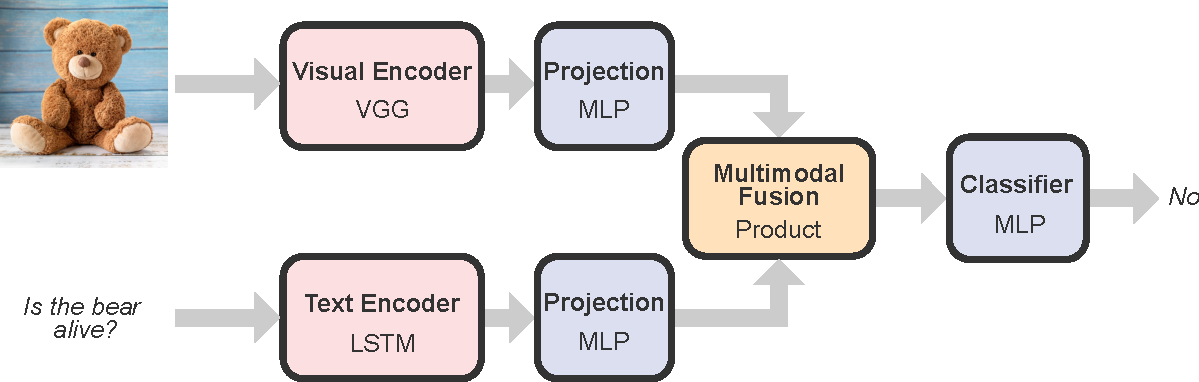
\includegraphics[width=0.8\textwidth]{Figures/Background/vqa_first.pdf}
\caption{First VQA architecture. Image and question embeddings are extracted and then projected to the same dimension. The result is then combined using the element-wise product, and a classifier provides the most likely answer at the output.}
\label{fig:vqa_first}
\end{center}
\end{figure}

Another breakthrough related to attention emerged with \gls{butd} attention~\cite{anderson2018bottom}, where grid features produced by a \gls{cnn} are replaced with object features produced by an \gls{r-cnn}~\cite{ren2015faster}. Attention is then computed along the region features to assign larger weights to the object regions that are more relevant to the question. Later on, \gls{ban} builds on the object-based feature extraction but proposes adding co-attention~\cite{xu2016ask} to \gls{mlb} with the aim of considering the interaction between every object region and every question word.

One of the early signs hinting at the upcoming transition to transformer-based architectures for \gls{vqa} was LXMERT~\cite{tan2019lxmert}. This model comprises three encoder blocks: one for text, one for object relationships, and one to combine both modalities. The cross-modality block has a special design containing a bidirectional cross-attention sub-layer constructed from two uni-directional cross-attention sub-layers, one from text to vision and one from vision to text. LXMERT is notable for being trained on various tasks, including language modeling, masked object prediction, image-text matching, and \gls{vqa}. Between 2020 and 2022, several approaches addressing different aspects of \gls{vqa} were proposed. These include investigating the relevance of grid features against region features~\cite{jiang2020defense}, learning with counterfactuals~\cite{liang2020learning}, data unshuffling~\cite{teney2020unshuffling}, and visual grounding~\cite{khan2021reason}.

Subsequently, the OFA model~\cite{wang2022ofa} emerged as an encoder-decoder transformer with up to 930M parameters, serving, together with Flamingo~\cite{alayrac2022flamingo}, as precursors to \glspl{mllm}, such as GPT-4V~\cite{achiam2023gpt}, BLIP-2~\cite{li2023blip2}, and Llama-adapters~\cite{zhang2023llamaadapter,gao2023llamaadapter}. A significant change introduced by these larger models is their ability to generate free-text answers instead of pre-defined ones, allowing for more varied responses and detailed descriptions.

As depicted in \fig~\ref{fig:vqa_evolution_background}, \glspl{mllm} mark a paradigm shift in the fundamental structure of the \gls{vqa} architecture. As discussed in Sec.~\ref{subsec:mllms}, in numerous state-of-the-art approaches, visual features are extracted with a visual encoder, mapped to the dimension of the language tokens, and then integrated with the language tokens. This facilitates the seamless utilization of the \gls{llm}, which can also be left frozen during the training process~\cite{guo2023images}. More recent advancements in \gls{vqa} focus on adding specialized world knowledge into the model~\cite{wang2024qa} and using synthetic questions to answer human questions~\cite{kim2024generalizing}. 

\subsubsection{Medical VQA}

In the medical domain, the evolution of \gls{medvqa} has closely paralleled the progress made for natural images, with some approaches being directly adapted to the medical domain. \gls{medvqa} is considered to have started later than general \gls{vqa} (see \fig~\ref{fig:vqa_evolution_background}), likely attributed, as mentioned earlier, to limited data availability and the associated annotation costs. The initiation of \gls{medvqa} was significantly influenced by the ImageCLEF VQA-Med challenge, inaugurated in 2018, marking the initial applications of \gls{vqa} to medical images. With a relatively small dataset with only 5,500 question-answer pairs for training, most of the approaches in the challenges were adapted from general \gls{vqa}, such as \gls{san}, \gls{mcb} and \gls{mfb}~\cite{ImageCLEFVQA_Med2018}. Addressing the challenge of limited data, a method was proposed in~\cite{nguyen2019overcoming}, utilizing meta-learning and a \gls{dae} to generalize in limited-data scenarios and exploit unlabeled images, respectively.

Two methods were then introduced for generating answers using different modules based on the type of question asked, either open-ended or close-ended~\cite{zhan2020medical,gupta2021hierarchical}. These practices posed a significant challenge in the early years of \gls{medvqa}, where certain methods were specifically tailored to the challenge data. Some approaches even treated the \gls{vqa} problem as an image classification problem, disregarding the input questions~\cite{al2020inception}. Fortunately, as new datasets emerged, approaches shifted focus towards other aspects, including enhancing the importance assigned to questions~\cite{vu2020question} and incorporating data augmentation techniques~\cite{gong2021cross}. From this point on, the adoption of transformer-based architectures, adapted from general \gls{vqa}, became prominent in \gls{medvqa}. This transition began with a pathology \gls{vqa} model that employed a transformer to fuse text and visual features~\cite{naseem2022vision}. Later, the integration of \glspl{mllm} into \gls{medvqa} has been observed~\cite{vansonsbeek2023openended,seenivasan2023surgicalgpt,he2024pefomed}.

\subsection{Datasets}
\label{sec:vqa_datasets}

In terms of datasets, significant differences exist between general and medical \gls{vqa}. \fig~\ref{fig:vqa_datasets_evolution} shows the most relevant datasets for natural and medical images over time. A notable characteristic of datasets in general \gls{vqa} is the refinement of earlier versions, exemplified by the progression from VQA v1~\cite{antol2015vqa} to VQA v2~\cite{goyal2017making}. Additionally, new versions like VQA-CP~\cite{agrawal2018don} were introduced to mitigate biases. This kind of dataset evolution is hardly observed in the medical domain, where, with some exceptions, there is only one version of the dataset. Due to the lack of data, challenges such as ImageCLEF VQA-Med have also re-used the same dataset used in previous versions~\cite{ImageCLEF-VQA-Med2021}.

\begin{figure}[t]
\begin{center}
\includegraphics[width=\textwidth]{Figures/Background/vqa_datasets_evolution.pdf}
\caption{Evolution of VQA datasets for natural and medical images over time. Dots with triangles and squares indicate datasets produced for a specific VQA challenge.}
\label{fig:vqa_datasets_evolution}
\end{center}
\end{figure}

Perhaps the most important dataset consideration is the number of images and question-answer pairs. As mentioned earlier, data collection in the medical domain is more challenging, resulting in substantially smaller datasets compared to their counterparts in general \gls{vqa}. 

To illustrate this, Table~\ref{tab:datasets_vqa} provides an overview of publicly available \gls{vqa} datasets for medical and natural images. Two conclusions can be drawn: (1) General \gls{vqa} datasets tend to contain more images and more questions than \gls{medvqa} datasets, and (2) \gls{medvqa} datasets often incorporate automatically generated questions. Both of these considerations can be seen as consequences of the difficulties associated with medical data, as presented in Sec.~\ref{subsec:vqa_vs_medvqa}. The first consideration impacts the quality of the models trained with such data, as achieving generalization becomes more challenging, making them more prone to biases. The second consideration limits the applicability or deployment of \gls{medvqa} models in clinical environments, primarily due to the disparity between the nature of automatically generated questions and human-generated questions. Generally, automatically generated questions tend to adhere to a fixed structure that does not fully capture the semantic and syntactic variability and complexity of questions posed by humans. 




\section{Basics of Diabetic Macular Edema (DME) Staging}

We briefly present basic concepts about fundus imaging and \gls{dme} staging due to its relevance in this thesis. \fig~\ref{fig:eye_anatomy} (left) shows the basic anatomy of the eye. This organ exhibits a layered organization crucial for vision. Light initially passes through the transparent cornea, refracting and entering the anterior chamber filled with aqueous humor. The iris, the pigmented structure visible as eye color, regulates the incoming light via the central pupil. The crystalline lens, located behind the iris, further focuses the light onto the retina, the light-sensitive layer lining the posterior chamber. Within the retina, photoreceptor cells, known as rods and cones, convert light energy into electrical signals. These signals are then transmitted through the optic nerve to the visual cortex in the brain, allowing for visual perception. The entire globe of the eye is encased by the tough, white sclera, providing structural support and protection. This intricate interplay of structures enables the eye to capture and process visual information, transforming light into the world we see~\cite{zhu2012eye}.

\begin{table}[ht]
\begin{center}
\begin{tabular}{lp{0.5cm}lp{0.5cm}lp{0.5cm}l}
\toprule
Dataset                       && \# Images         && \# Questions && QA creation \\ \midrule
E-VQA~\cite{yang2023event} && 2,690 && 9,088 && Automatic \\
OK-VQA~\cite{marino2019okvqa}   && 14,031           && 14,055 && Manual \\
VizWiz 2018~\cite{gurari2018vizwiz} && 21,173 && 31,173 && Manual \\
TextVQA~\cite{singh2019towards}   && 28,408           && 45,336 && Manual\\ 
DocVQA~\cite{mathew2021docvqa}   && 12,000           && 50,000 && Manual \\
LoRA~\cite{gao2024lora} && 100,00 && 200,000 && Automatic\\
Visual7W~\cite{zhu2016visual7w}  && 47,300 && 327,929 && Manual \\ 
VQA-CPv1~\cite{agrawal2018don}   && 205,000           && 370,000  && Manual\\
VQAv1~\cite{antol2015vqa}      && 204,721    && 614,163    && Manual  \\ 
VQA-CPv2~\cite{agrawal2018don}   && 219,000          && 658,000  && Manual\\
CLEVR~\cite{johnson2017clevr}   && 100,000 && 864,968   && Automatic \\ 
VQAv2~\cite{goyal2017making}   && 204,721 && 1'105,904 && Manual \\ 
GQA~\cite{hudson2019gqa}  && 113,000           && 22'000,000   &&  Automatic \\ \midrule
RadVisDial (gold)~\cite{kovaleva2020towards}  && 100 && 500 &&  Manual \\ 
VQA-RAD~\cite{lau2018dataset}  && 316 && 3,515 && Manual \\ 
VQA-Med 2020~\cite{ImageCLEF-VQA-Med2020}  && 5,000    &&  5,000 &&  Automatic   \\  
VQA-Med 2021~\cite{ImageCLEF-VQA-Med2021}  && 5,000 && 5,000 && Automatic \\ 
VQA-Med 2018~\cite{ImageCLEFVQA_Med2018} && 2,866    &&   6,413  && Automatic   \\  
DME-VQA~\cite{tascon2022consistency} && 679 && 12,159 && Automatic \\
Slake~\cite{liu2021slake}  && 642 && 14,000 && Manual \\
VQA-Med 2019~\cite{ImageCLEFVQA-Med2019}   && 4,200 &&  15,292 && Automatic \\ 
VQA-Med 2023~\cite{ImageCLEF2023}  && 5,000 && 25,000 && Automatic \\ 
PathVQA~\cite{he2020pathvqa}  && 4,998 && 32,799 && Automatic\\ 
PMC-VQA~\cite{zhang2023pmc}  && 149,000 && 227,000 && Automatic\\ 
RadVisDial (silver)~\cite{kovaleva2020towards}  && 91,060 && 455,300 &&  Automatic \\ \bottomrule
\end{tabular}
\end{center}
\caption{Overview of VQA dataset size sorted by the number of questions. \textbf{Top:} For natural images. \textbf{Bottom:} For medical images.}
\label{tab:datasets_vqa}
\end{table}

\begin{figure}[h]
\begin{center}
\includegraphics[width=\textwidth]{Figures/Background/anatomy_fundus.png}
\caption{\textbf{Left:} Anatomy of the eye (from~\cite{sightresearchukYourEyes}). \textbf{Right:} Fundus image from the IDRiD dataset~\cite{idrid} with hard exudates encircled in light blue.}
\label{fig:eye_anatomy}
\end{center}
\end{figure}

\subsection{Fundus Imaging}

In \gls{dme} risk grade diagnosis from fundus images we are interested in capturing the rear of the eye, which is also known as fundus. This requires a specialized camera focused on the eye while emitting a bright light source, typically a flash or an infrared beam. The light travels through the eye, as described before, and reflects off the structures at the back of the eye and travels back through the pupil. A series of mirrors and lenses within the camera capture and concentrate this reflected light.
Modern fundus cameras are digital, capturing an image directly onto a sensor instead of using film~\cite{bernardes2011digital}. 


\subsection{DME Staging}

In assessing the severity of \gls{dme} through color fundus images, a simplified classification system utilizes a three-point scale (0-2) to categorize disease progression. Grade 0 signifies a healthy retina, devoid of any visible "hard exudates," which appear as yellowish-white deposits. Grade 1 indicates the presence of these deposits confined to the peripheral regions of the retina, outside the central "macular area." Conversely, Grade 2 denotes the presence of hard exudates within the critical macular region, raising potential concerns for vision impairment. For practical purposes, the critical macular region is defined by a circle with a radius of one optic disc diameter~\cite{ren2018diabetic}. \fig~\ref{fig:eye_anatomy} (right) shows an example where hard exudates are within this critical region, leading to Grade 2.

\part{Enabling Localized Queries in VQA}
\label{part:localized}
\chapter{Localized Questions in Medical Visual Question Answering}
\label{chapter:locvqa}
% MICCAI 2023 paper about localized questions

The task of \gls{vqa} has seen a relatively rapid development since it was first introduced back in 2015. With a few exceptions, \gls{vqa} models have been applied to datasets with questions that refer to the entire image. This, however, can limit the interpretability of the model's predictions, as the model can benefit from biases in the data to produce the correct answer while disregarding the parts of the image that contain key information to answer the question. Furthermore, localized questions allow the comparison and quantification of agreement between questions about images and questions about regions. In this work, we present an attention-based method for medical \gls{vqa} that enables the posing of questions about specific user-defined regions of an image while considering the context required to answer them. We benchmark our approach across multiple datasets and against different baselines, showing its effectiveness. 

\textbf{Author Contribution} The contributing authors to this work are Pablo Márquez-Neila and Raphael Sznitman. My contributions to this chapter include the creation of the datasets, the development of the methodology, the conception and realization of the experiments, data analysis and interpretation, and visualization as well as the writing of the manuscript.

\textbf{Publication}  This work is published in the Proceedings of the MICCAI 2023 conference \cite{tascon2023localized}.

\newpage

% Paper contents
\section{Background and Previous Work}
\label{sec:locvqa_locatt_background}

\gls{vqa} models are neural networks that answer natural language questions about an image~\cite{antol2015vqa,goyal2017making,hudson2019gqa,tan2019lxmert}. The capability of \gls{vqa} models to interpret natural language questions is of great appeal, as the range of possible questions that can be asked is vast and can differ from those used to train the models. This has led to many proposed \gls{vqa} models for medical applications in recent years~\cite{ImageCLEFVQA_Med2018,liu2019effective,liao2020aiml,vu2020question,zhan2020medical,gong2021cross,yu2023question}. These models can enable clinicians to probe the model with nuanced questions, thus helping to build confidence in its predictions.

Recent work on \gls{medvqa} has primarily focused on building more effective model architectures~\cite{gong2021cross,ren2020cgmvqa,vu2020question} or developing strategies to overcome limitations in \gls{medvqa} datasets~\cite{Nguyen19,liu2021slake,pelka2018radiology,do2021multiple,vu2020question}. Another emerging trend is to enhance \gls{vqa} performance by addressing the consistency of answers produced~\cite{tascon2022consistency}, particularly when considering entailment questions (\ie, the answer to ``Is the image that of a healthy subject?" should be consistent with the answer to ``Is there a fracture in the tibia?"). Despite these recent advances, however, most \gls{vqa} models are restricted to questions that consider the entire image at a time. Specifically, \gls{vqa} typically uses questions that address content within an image without specifying where this content may or may not be in the image. Yet the ability to ask specific questions about regions or locations of the image would be highly beneficial to any user as it would allow fine-grained questions and model probing. For instance, Fig.~\ref{fig:examples_data} illustrates examples of such \emph{localized questions} that combine content and spatial specifications. In the medical field, posing localized questions can significantly enhance the diagnostic process by providing second opinions to medical experts about suspicious regions. Additionally, this approach can improve trustworthiness by assessing the consistency between answers to both global and localized questions.

To this day, few works have addressed the ability to include location information in \gls{vqa} models. In~\cite{mani2020point}, localization information is posed in questions by constraining the spatial extent to a point within bounding boxes yielded by an object detector. The model then focuses its attention on objects close to this point. However, the method was developed for natural images and relies heavily on the object detector to limit the attention extent, making it difficult to scale in medical imaging applications. Alternatively, the approach from~\cite{vu2020question} answers questions about a pre-defined coarse grid of regions by directly including region information into the question (\eg, ``Is grasper in (0,0) to~(32,32)?"). This method relies on the ability of the model to learn a spatial mapping of the image and limits the regions to be on a fixed grid. Localized questions were also considered in~\cite{tascon2022consistency}, but the region of interest was cropped before being presented to the model, assuming that the surrounding context is irrelevant for answering this type of question.
\begin{figure}[!t]
\begin{center}
\includegraphics[width=0.9\textwidth]{Figures/Part1_LocVQA/01_locatt/examples_data.pdf}
\caption{Examples of localized questions. In some cases (RIS-VQA and INSEGCAT-VQA), the object mentioned in the question is only partially present in the region. We hypothesize that context can play an important role in answering such questions.}
\label{fig:examples_data}
\end{center}
\end{figure}

To overcome these limitations, we propose a novel \gls{vqa} architecture that alleviates the mentioned issues. At its core, we hypothesize that by allowing the \gls{vqa} model to access the entire images and properly encoding the region of interest, this model can be more effective at answering questions about regions. To achieve this, we propose using a multi-glimpse attention mechanism~\cite{ben2017mutan,vu2020question,tascon2022consistency} restricting its focus range to the region in question, but only after the model has considered the entire image. By doing so, we preserve contextual information about the question and its region. We evaluate the effectiveness of our approach by conducting extensive experiments on three datasets and comparing our method to state-of-the-art baselines. Our results demonstrate performance improvements across all datasets. 
\section{Method}
\label{sec:locvqa_locatt_method}

Our method extends a \gls{vqa} model to answer localized questions. We define a \emph{localized question} for an image~$\x$ as a tuple~$(\q, \m)$, where $\q$~is a question, and $\m$~is a binary mask of the same size as~$\x$ that identifies the region to which the question pertains. Our \gls{vqa} model, parameterized by $\bm{\theta}$ and depicted in Fig.~\ref{fig:method_locvqa}, accepts an image and a localized question as input and produces a probability distribution over a finite set~$\mathcal{A}$ of possible answers. The final answer~$\hat{a}$ of the model is the element with the highest probability,
\begin{equation}
    \hat{a} = \argmax_{a\in\mathcal{A}} p(a\mid \q, \x, \m; \bm{\theta}).
\end{equation}
The model proceeds in three stages to produce its prediction: input embedding, localized attention, and final classification.

\subsection{Input Embedding} The question~$\q$ is first processed by an \gls{lstm}~\cite{hochreiter1997long} to produce an embedding~$\hat{\q}\in\real^Q$. Similarly, the image~$\x$ is processed by a ResNet-152~\cite{he2016deep} to produce the feature map~$\hat{\x}\in\real^{C\times{}H\times{}W}$.

\subsection{Localized Attention} An attention mechanism uses the embedding to determine relevant parts of the image to answer the corresponding question. Unlike previous attention methods, we include the region information that the mask defines. Our \emph{localized attention} module (Fig.~\ref{fig:method_locvqa} right) uses both descriptors and the mask to produce multiple weighted versions of the image feature map,~$\hat{\x}'=\att(\hat{\q}, \hat{\x}, \m)$. To do so, the module first computes an attention map~$\g\in\real^{G\times{}H\times{}W}$ with $G$~glimpses by applying unmasked attention~\cite{kim2016hadamard,vu2020question} to the image feature map and the text descriptor. The value of the attention map at location~$(h, w)$ is computed as,
\begin{equation}
    \g_{:hw} = \textrm{softmax}\left(\W^{(g)}\cdot\textrm{ReLU}\left(\W^{(x)}\hat{\x}_{:hw} \odot \W^{(q)}\hat{\q}\right)\right),
\end{equation}
where the index ${:}hw$ indicates the feature vector at location~$(h, w)$, $\W^{(x)}\in\real^{C'\times C}$, $\W^{(q)}\in\real^{C'\times Q}$, and $\W^{(g)}\in\real^{G\times C'}$ are learnable parameters of linear transformations, and $\odot$~is the element-wise product. In practice, the transformations $\W^{(x)}$ and $\W^{(g)}$ are implemented with $1\times{}1$~convolutions and all linear transformations include a dropout layer applied to its input. The image feature maps~$\hat{\x}$ are then weighted with the attention map and masked with~$\m$ as,
\begin{equation}
    \hat{\x}'_{cghw} = \g_{ghw} \cdot \hat{\x}_{chw} \cdot \left(\m\downarrow_{H\times{}W}\right)_{hw},
\end{equation}
where $c$ and~$g$ are the indexes over feature channels and glimpses, respectively, $(h, w)$~is the index over the spatial dimensions, and $\m\downarrow_{H\times{}W}$~denotes a binary downsampled version of~$\m$ with the spatial size of~$\hat{\x}$. This design allows the localized attention module to compute the attention maps using the full information available in the image, thereby incorporating context into them before being masked to constrain the answer to the specified region.

\subsection{Classification} The question descriptor~$\hat{\q}$ and the weighted feature maps~$\hat{\x}'$ from the localized attention are vectorized and concatenated into a single vector of size~$C\cdot{}G + Q$ and then processed by a multi-layer perceptron classifier to produce the final probabilities.

\subsection{Training} The training procedure minimizes the standard cross-entropy loss over the training set updating the parameters of the \gls{lstm} encoder, localized attention module, and the final classifier. The training set consists of triplets of images, localized questions, and the corresponding ground-truth answers. As in~\cite{antol2015vqa}, the ResNet weights are fixed with pre-trained values, and the \gls{lstm} weights are updated during training.

\begin{figure}[!t]
\begin{center}
\includegraphics[width=0.99\textwidth]{Figures/Part1_LocVQA/01_locatt/method_new.pdf}
\caption{\textbf{Left:} Proposed VQA architecture for localized questions. The Localized Attention module allows the region information to be integrated into the VQA while considering the context necessary to answer the question. \textbf{Right:} Localized Attention module.  
}
\label{fig:method_locvqa}
\end{center}
\end{figure}
\section{Experiments and Results}
\label{sec:locvqa_locatt_experiments_and_results}

We compare our model to several baselines across three datasets and report quantitative and qualitative results. Additional results are available in Appendix~\ref{appendix:locvqa}. 

\subsection{Datasets}
\label{subsec:locvqa_datasets}
We evaluate our method on three datasets containing questions about regions which we detail here. The first dataset consists of an existing retinal fundus \gls{vqa} dataset with questions about the image's regions and the entire image. The second and third datasets are generated from public segmentation datasets but  use the method described in~\cite{vu2020question} to generate a \gls{vqa} version with region questions. %Fig.~\ref{fig:examples_data} illustrates examples of question-answer pairs in these datasets which we describe in more detail here:
\begin{description}
    \item[\gls{dme}-VQA~\cite{tascon2022consistency}:] 679~fundus images containing questions about entire images (\eg,~``what is the \gls{dme} risk grade?") and about randomly generated circular regions (\eg,~``are there hard exudates in this region?"). The dataset comprises 9'779~question-answer~(QA) pairs for training, 2'380~for validation, and 1'311 for testing.
    \item[RIS-VQA:] Images from the 2017~Robotic Instrument Segmentation dataset~\cite{allan20192017}. We automatically generated binary questions with the structure ``is there [instrument] in this region?" and corresponding masks as rectangular regions with random locations and sizes. Based on the ground-truth label maps, the binary answers were labeled ``yes'' if the region contained at least one pixel of the corresponding instrument and ``no'' otherwise. The questions were balanced to maintain the same amount of ``yes'' and ``no'' answers. 15'580~QA pairs from 1'423 images were used for training, 3'930 from 355 images for validation, and 13'052 from 1'200 images for testing.
    %Though not reported in the paper, we also experimented with other thresholds to define positive answers. For example, making the threshold dependent on region area (1\%), or by using 10 px as threshold. In both cases, we observed significantly better performance in our method. For example, using the mentioned thresholds on the RIS-VQA dataset, our method has an AUC 0.04 higher than the baseline Crop Region, which is very similar to the difference reported in the paper (0.05). We considered 1 px the least arbitrary threshold and reported results for it
    \item[INSEGCAT-VQA:] Frames of cataract surgery videos from the InSegCat~2 dataset~\cite{fox2020insegcat}. We followed the same procedure as in RIS-VQA to generate balanced binary questions with masks and answers.
    The dataset consists of 29'380~QA pairs from 3'519 images for training, 5'306 from 536 images for validation, and 4'322 from 592 images for testing. % also in this case with 50\% Yes and 50\% No questions. 
\end{description}
Fig.~\ref{fig:object_distribution} shows the distribution of questions in the three datasets.

\begin{figure}[t]
\begin{center}
\includegraphics[width=\textwidth]{Figures/Part1_LocVQA/01_locatt/pie_charts_data.pdf}
\caption{Distribution by question type (DME-VQA) and by question object (RIS-VQA and INSEGCAT-VQA).}
\label{fig:object_distribution}
\end{center}
\end{figure}

\subsection{Baselines and Metrics}
We compare our method to four different baselines, as shown in Fig.~\ref{fig:baselines}:
\begin{description}
    \item[No mask:] no information is provided about the region in the question.
    \item[Region in text~\cite{vu2020question}:] region information is included as text in the question.
    \item[Crop region~\cite{tascon2022consistency}:] image is masked to show only the queried region, with the area outside the region set to zero.
    \item[Draw region:] region is indicated by drawing its boundary on the input image with a distinctive color.
\end{description}
We evaluated the performance of our method using accuracy for the DME-VQA dataset and the area under the \gls{roc} curve and Average Precision (AP) for the RIS-VQA and INSEGCAT-VQA datasets.

\begin{figure}[!t]
\begin{center}
\includegraphics[width=0.98\textwidth]{Figures/Part1_LocVQA/01_locatt/baselines.pdf}
\caption{Illustration of the evaluated baselines for an example image.}
\label{fig:baselines}
\end{center}
\end{figure}

\subsubsection{Implementation Details}

Our \gls{vqa} architecture uses an \gls{lstm}~\cite{hochreiter1997long} with an output dimension~1024 to encode the question and a word embedding size of~300.
% The question length is~12 for normal questions and 21 when the region information is included in the question \PMN{Why do we need to specify this? It sounds strange that we have two exact kinds of questions.}. \STM{Questions with region info are naturally longer, so they require a bigger vector size. It's not essential to mention it.} 
We use the ResNet-152~\cite{he2016deep} with ImageNet weights to encode images of size 448$\times$448, generating feature maps with 2048~channels.
% For multimodal fusion, we use concatenation.
In the localized attention block, the visual and textual features are projected into a 512-dimensional space before being combined by element-wise multiplication. Following \cite{fukui2016multimodal,kim2016hadamard}, the number of glimpses is set to $G=2$ for all experiments.
The classification block is a multi-layer perceptron with a hidden layer of~1024 dimensions. A dropout rate of~0.25 and \gls{relu} activation are used in the localized attention and classifier blocks.

We train our models for 100~epochs using an early stopping condition with patience of 20~epochs. Data augmentation consists of horizontal flips. We use a batch size of 64~samples and the Adam optimizer with a learning rate of $10^{-4}$, which is reduced by a factor of 0.1 when learning stagnates.
% For the DME-VQA dataset, we used weighted cross-entropy, and for the other datasets, we used binary cross-entropy.
Models implemented in PyTorch 1.13.1 and trained on an Nvidia RTX 3090 graphics card\footnote{Our code and data are available at \url{https://github.com/sergiotasconmorales/locvqa}}. 

%%%%%%%%%%%%%%%%%%%%%%%%%%%%%%%
% Results                     %
%%%%%%%%%%%%%%%%%%%%%%%%%%%%%%%

\subsection{Results} 

\label{sec:locvqa_results}


% Table~\ref{tab:locvqa_results_dme} summarizes the results obtained on the DME-VQA dataset for all methods and each type of question. Table~\ref{tab:results_ris_insegcat} shows the RIS-VQA and INSEGCAT-VQA datasets results. Additionally, Table~\ref{tab:results_ris_object} reports the performances for questions pertaining to each type of instrument in the RIS-VQA dataset.  

\begin{table}[!t]
\begin{center}
\begin{tabular}{llp{0.1cm}lp{0.1cm}lp{0.1cm}lp{0.1cm}c}
%
\toprule
\multicolumn{1}{l}{\multirow{2}{*}{Method}} & \multicolumn{9}{c}{Accuracy (\%)}                                                                                                                                               \\ \cmidrule{2-10} 
\multicolumn{1}{c}{} & \multicolumn{1}{c}{Overall}      && \multicolumn{1}{c}{Grade}        && \multicolumn{1}{c}{Whole}        && \multicolumn{1}{c}{Macula}       && \multicolumn{1}{c}{Region} \\ \midrule 
No Mask & \multicolumn{1}{c}{61.1 $\pm$ 0.4} && \multicolumn{1}{c}{80.0 $\pm$ 3.7} && \multicolumn{1}{c}{85.7 $\pm$ 1.2} && \multicolumn{1}{c}{\textbf{84.3 $\pm$ 0.5}} && 57.6 $\pm$ 0.4                \\ 
Region in Text~\cite{vu2020question} & \multicolumn{1}{c}{ 60.0 $\pm$ 1.5} && \multicolumn{1}{c}{57.9 $\pm$ 12.5 } && \multicolumn{1}{c}{85.1 $\pm$ 1.9 } && \multicolumn{1}{c}{ 83.2 $\pm$ 2.4} &&     57.7 $\pm$ 1.0        \\ 
Crop Region~\cite{tascon2022consistency}  & \multicolumn{1}{c}{81.4 $\pm$ 0.3} && \multicolumn{1}{c}{78.7 $\pm$ 1.3} && \multicolumn{1}{c}{81.3 $\pm$ 1.7} && \multicolumn{1}{c}{82.3 $\pm$ 1.4} && 81.5 $\pm$ 0.3               \\
Draw Region  & \multicolumn{1}{c}{ 83.0 $\pm$ 1.0} && \multicolumn{1}{c}{79.6 $\pm$ 2.5 } && \multicolumn{1}{c}{77.0 $\pm$ 4.8 } && \multicolumn{1}{c}{84.0 $\pm$ 1.9 } &&   83.5 $\pm$ 1.0               \\ 
\ours                                          & \multicolumn{1}{c}{\textbf{84.2 $\pm$ 0.6}} && \multicolumn{1}{c}{\textbf{82.8 $\pm$ 0.4}} && \multicolumn{1}{c}{\textbf{87.0 $\pm$ 1.2}} && \multicolumn{1}{c}{83.0 $\pm$ 1.5} && \textbf{84.2 $\pm$ 0.7}                \\ \bottomrule
\end{tabular}
\end{center}
\caption{Average accuracy for different methods on the DME-VQA dataset. The results shown are the average of 5 models trained with different seeds.}
\label{tab:locvqa_results_dme}
\end{table}


\begin{table}[!t]
\begin{center}
\begin{tabular}{lp{0.5cm}lp{0.5cm}cp{0.5cm}c}
\toprule
Dataset                       && Method         && AUC && AP \\ \midrule
\multirow{4}{*}{RIS-VQA}      && No Mask    && 0.500 $\pm$ 0.000    &&  0.500 $\pm$ 0.000  \\ 
                                && Region in Text~\cite{vu2020question} &&  0.677 $\pm$ 0.002 && 0.655 $\pm$ 0.003 \\ 
                              && Crop Region~\cite{tascon2022consistency}    &&  0.842 $\pm$ 0.002 && 0.831 $\pm$ 0.002      \\  
                              && Draw Region && 0.835 $\pm$ 0.003 && 0.829 $\pm$ 0.003 \\ 
                              && \ours           && \textbf{0.885 $\pm$ 0.003} && \textbf{0.885 $\pm$ 0.003}\\ \midrule
\multirow{4}{*}{INSEGCAT-VQA} && No Mask    &&   0.500 $\pm$ 0.000  &&  0.500 $\pm$ 0.000   \\  
                              && Region in Text~\cite{vu2020question} &&  0.801 $\pm$ 0.012 && 0.793 $\pm$ 0.014 \\ 
                              && Crop Region~\cite{tascon2022consistency}    &&  0.901 $\pm$ 0.002   && 0.891 $\pm$ 0.003   \\  
                              && Draw Region && 0.910 $\pm$ 0.003 && 0.907 $\pm$ 0.005\\  
                              && \ours           &&  \textbf{0.914 $\pm$ 0.002}   && \textbf{0.915 $\pm$ 0.002}   \\ \bottomrule
\end{tabular}
\end{center}
\caption{Average test AUC and AP for different methods on the RIS-VQA and INSEGCAT-VQA datasets. The results shown are the average over 5~seeds.}
\label{tab:results_ris_insegcat}
\end{table}

\begin{table}[!t]
\ra{1.2}
\begin{center}
\begin{tabular}{p{0.1cm}p{0.13\linewidth}p{0.3cm}LKLKLK}
\toprule
{} &\multirow{2}{*}{Method}  & \multicolumn{7}{c}{Instrument Type} \\
\cmidrule{3-9} 
&         && Large Needle Driver & Monopolar Curved Scissors & Vessel Sealer & Grasping Retractor & Prograsp Forceps & Bipolar Forceps \\ \midrule
&\makecell[tl]{No\\Mask}    && \makecell[tc]{0.500 \\ $\pm$0}              & \makecell[tc]{0.500 \\ $\pm$0}                     & \makecell[tc]{0.500 \\ $\pm$0}            & \makecell[tc]{0.500 \\$\pm$0}                 & \makecell[tc]{0.500 \\ $\pm$0}              & \makecell[tc]{0.500 \\ $\pm$0}              \\ 
&\makecell[tl]{Region in\\Text~\cite{vu2020question}} &&   \makecell[tc]{0.717\\$\pm$0.003}                  &   \makecell[tc]{0.674\\$\pm$0.001}                        &     \makecell[tc]{0.620\\$\pm$0.011}          &    \makecell[tc]{0.616\\$\pm$0.020}                &    \makecell[tc]{0.647\\$\pm$0.008}              &  \makecell[tc]{0.645\\$\pm$0.003}               \\ 
&\makecell[tl]{Crop\\Region~\cite{tascon2022consistency}}    && \makecell[tc]{0.913 \\$\pm$0.002}               & \makecell[tc]{0.812 \\$\pm$0.003}                     & \makecell[tc]{0.752\\$\pm$0.009}         & \makecell[tc]{0.715\\$\pm$0.015}              & \makecell[tc]{0.773 \\$\pm$0.003}            & \makecell[tc]{0.798 \\$\pm$0.004}           \\ 
&\makecell[tl]{Draw\\Region} &&       \makecell[tc]{0.915\\$\pm$0.003}              &   \makecell[tc]{0.777\\$\pm$0.003}       &   \makecell[tc]{0.783\\$\pm$0.004}      &  \makecell[tc]{0.709\\$\pm$0.012}       &  \makecell[tc]{0.755\\$\pm$0.004}       &     \makecell[tc]{0.805\\$\pm$0.005}            \\ 
&\ours          && \makecell[tc]{\textbf{0.944}\\$\pm$\textbf{0.001}}               & \makecell[tc]{\textbf{0.837} \\$\pm$\textbf{0.005}}                     & \makecell[tc]{\textbf{0.872} \\$\pm$\textbf{0.008}}         & \makecell[tc]{\textbf{0.720} \\$\pm$\textbf{0.031}}              & \makecell[tc]{\textbf{0.834} \\$\pm$\textbf{0.006}}            & \makecell[tc]{\textbf{0.880} \\$\pm$\textbf{0.003}}           
\\ \bottomrule
\end{tabular}
\end{center}
\caption{Average test AUC for different methods on the RIS-VQA dataset as a function of instrument type. Results are averaged over 5 models trained with different seeds. The corresponding table for INSEGCAT-VQA is available in Appendix~\ref{appendix:locvqa}.
}
\label{tab:results_ris_object}
\end{table}

Our method outperformed all considered baselines on the DME-VQA (Table~\ref{tab:locvqa_results_dme}), the RIS-VQA, and the INSEGCAT-VQA datasets (Table~\ref{tab:results_ris_insegcat}), highlighting the importance of contextual information in answering localized questions. Context proved to be particularly critical in distinguishing between objects of similar appearance, such as the bipolar and prograsp forceps in RIS-VQA, where our method led to an 8~percent point performance improvement (Table~\ref{tab:results_ris_object}). In contrast, the importance of context was reduced when dealing with visually distinct objects, resulting in smaller performance gains as observed in the INSEGCAT-VQA dataset. For example, despite not incorporating contextual information, the baseline \emph{crop region} still benefited from correlations between the location of the region and the instrument mentioned in the question (\eg,~the eye retractor typically appears at the top or the bottom of the image), enabling it to achieve competitive performance levels that are less than 2~percent points lower than our method~(Table~\ref{tab:results_ris_insegcat}, bottom).

% Across the different datasets, we see that our approach consistently provides performance improvements. This highlights the importance of context in answering localized questions but also depends on how necessary context is to differentiate between all the objects that can be asked about. For instance, we notice that questions that involve objects with similar aspects (\eg, bipolar and prograsp forceps in RIS-VQA) can benefit more from context. In contrast, when an object is notably different from every other object in the scene (\eg, hard exudates in DME-VQA), the boost in performance is limited. This is observed especially in the INSEGCAT-VQA, in which the visual similarity of the tools is rather low and where the model that does not have access to context appears to benefit from correlations between the region location and the object mentioned in the question (\eg, the eye retractor appears at the top or the bottom of the image).

Similar to our method, the baseline \emph{draw region} incorporates contextual information when answering localized questions. However, we observed that drawing regions on the image can interfere with the computation of guided attention maps, leading to incorrect predictions (Fig.~\ref{fig:examples_att}, column~4). In addition, the lack of masking of the attention maps often led the model to wrongly consider areas beyond the region of interest while answering questions~(Fig.~\ref{fig:examples_att}, column~1). 

When analyzing mistakes made by our model, we observe that they tend to occur when objects or background structures in the image look similar to the object mentioned in the question~(Fig.~\ref{fig:examples_att}, column~3). Similarly, false predictions were observed when only a few pixels of the object mentioned in the question were present in the region.


%the model confuses other objects or tissue with the referred object or when the attention maps do not focus on the actual referred object \PMN{These two reasons say that the model fails when it is confused, which is a bit of a circular reasoning. What are the properties of the images that make the model fail? Do they have something in common?} \STM{They tend to contain tissue that has the shape of tools, for example. Or they contain two very similar tools. Or only a very small portion of the object is in the region. This of course doesn't explain all errors, but that's what I saw in common} \PMN{Also, we are only showing a single failure example, which might be not enough.} \STM{Added one more failure from INSEGCAT and transposed the image to use the space better} (Fig.~\ref{fig:examples_att}, column~3).

% to analyze:
% Importance of context when questions require context + without context model confuses other objects with objects mentioned in the question (first row of examples figure)
% Why our method is better than drawing the regions (drawn regions can interfere in attention maps)
% Errors are still possible while considering context

\begin{figure}[!t]
\begin{center}
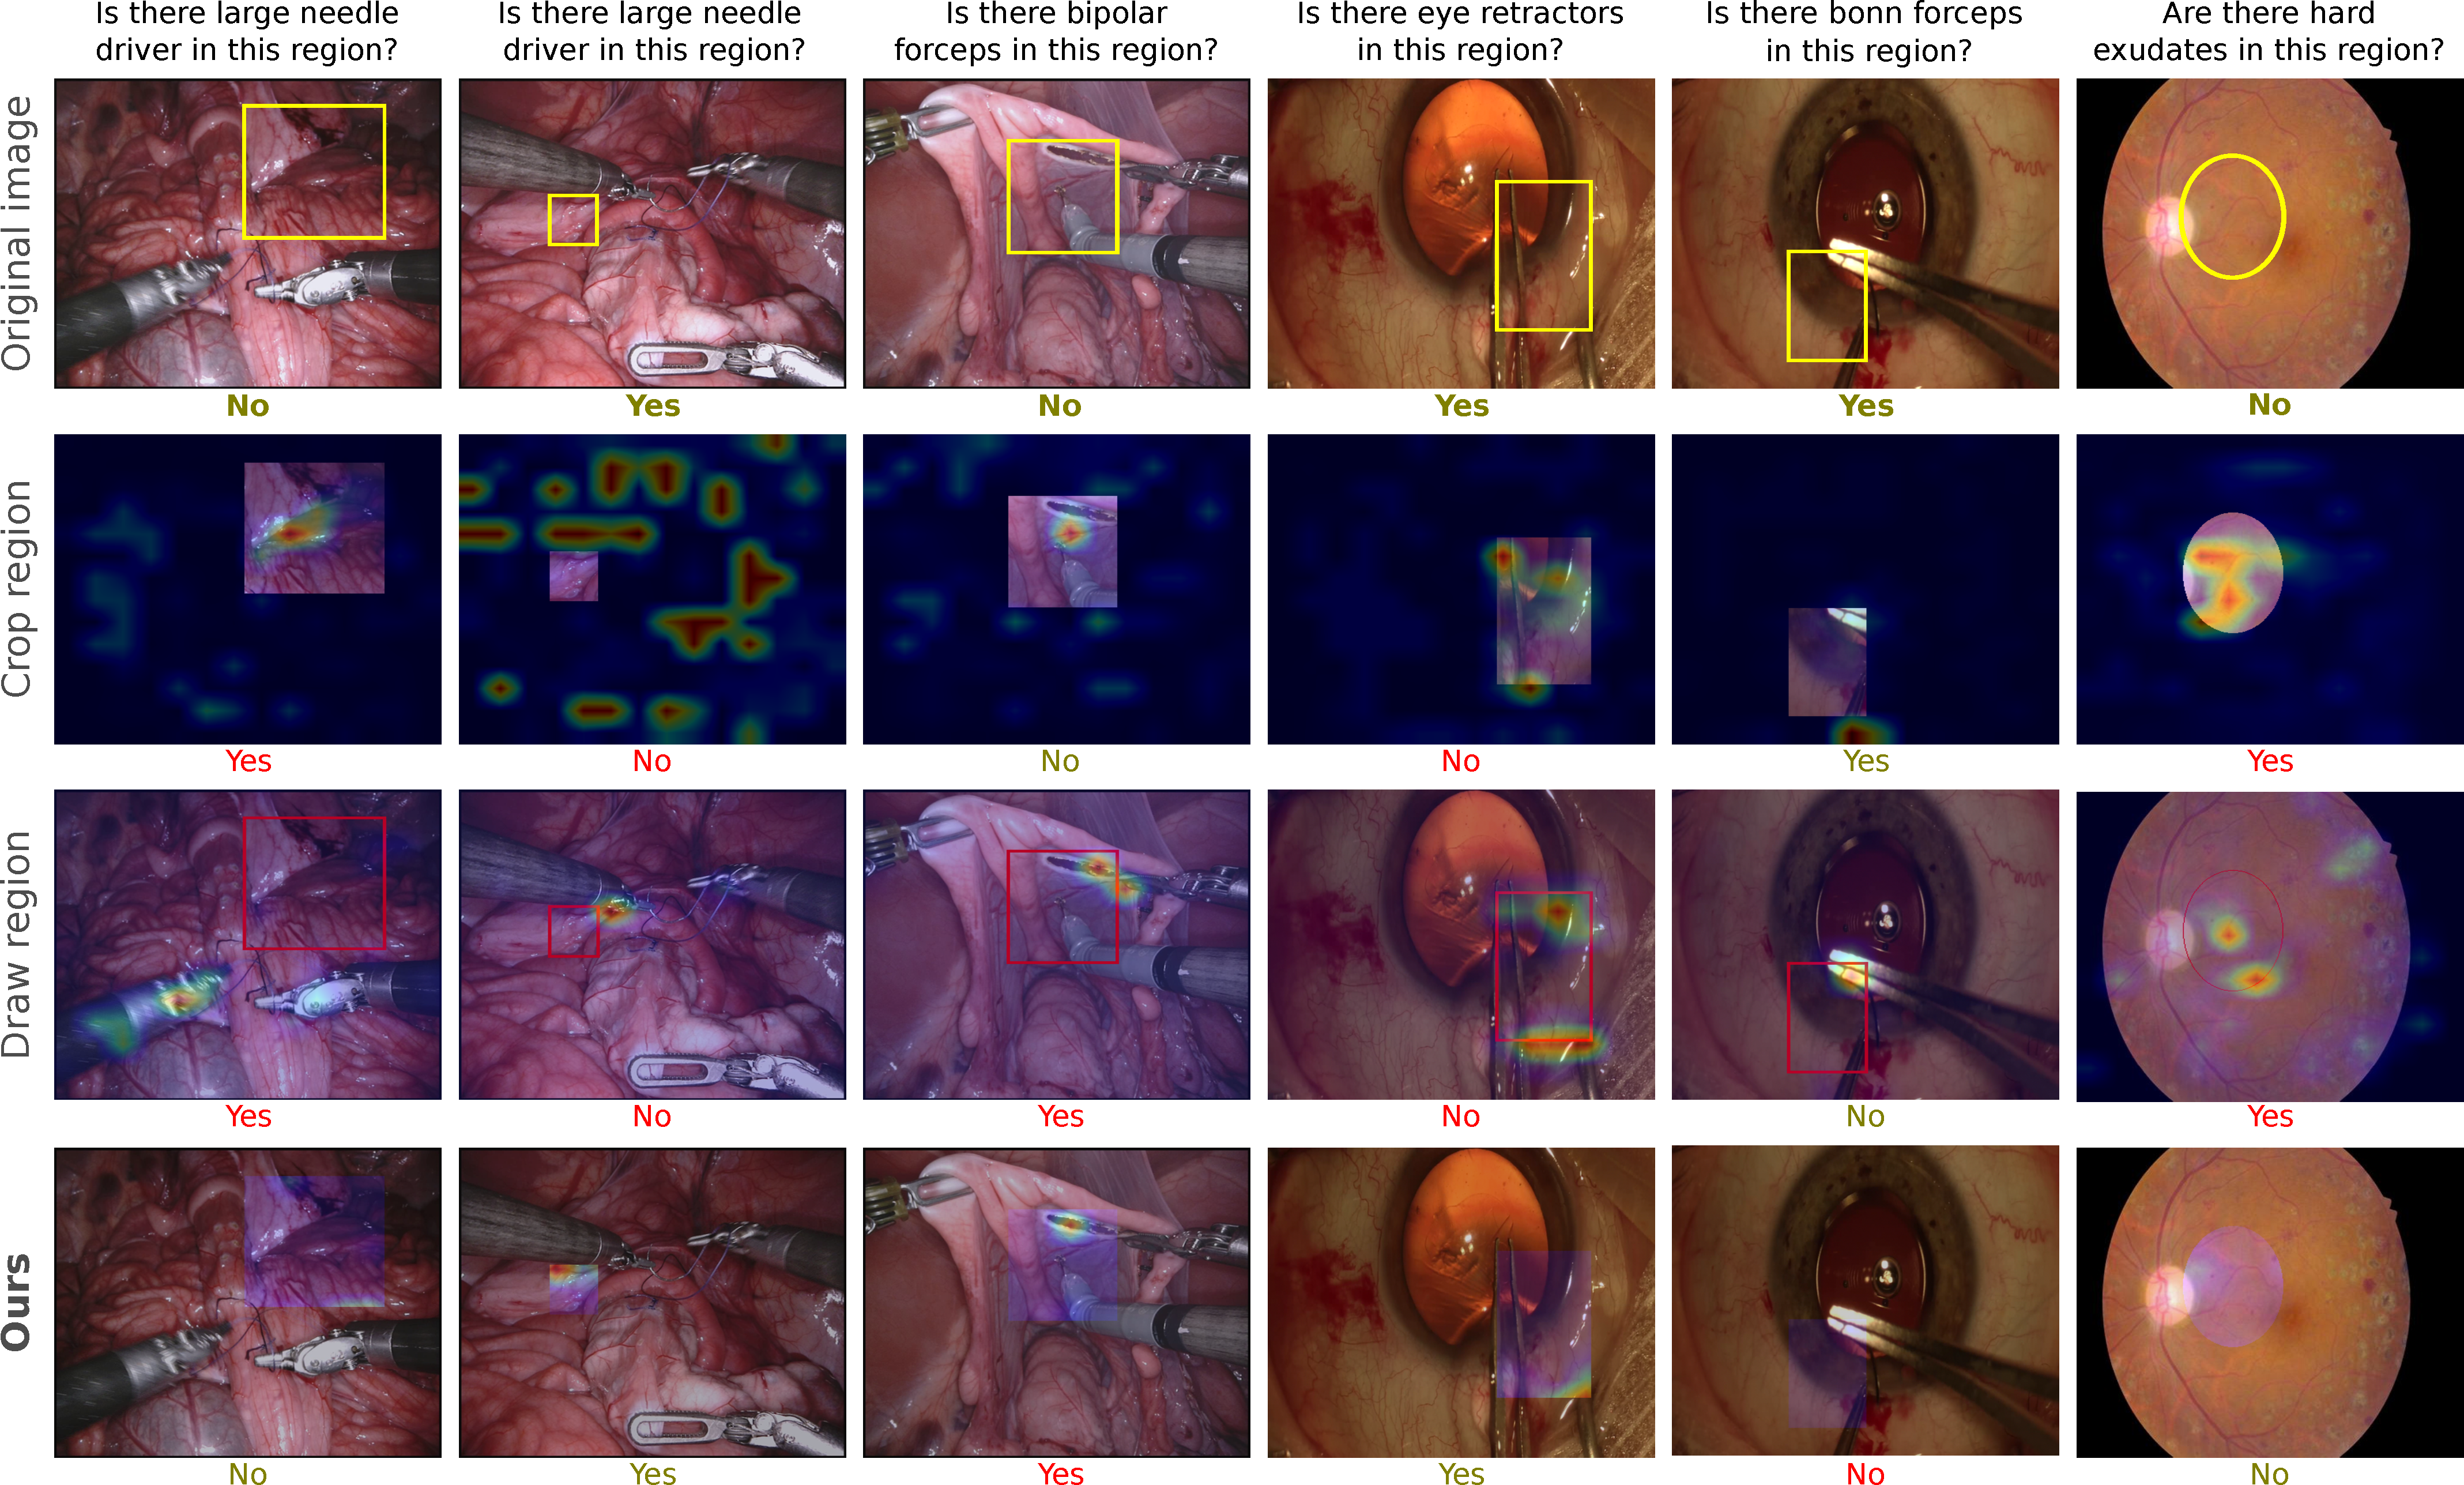
\includegraphics[width=\textwidth]{Figures/Part1_LocVQA/01_locatt/examples_att_small2_transposed.pdf}
\caption{Qualitative examples on the RIS-VQA dataset (columns~1-3), INSEGCAT-VQA (columns~4-5), and DME-VQA (last column). Only the strongest baselines were considered in this comparison. The first row shows the image, the region, and the ground truth answer. Other rows show the overlaid attention maps and the answers produced by each model. Wrong answers are shown in red.}
\label{fig:examples_att}
\end{center}
\end{figure}
\section{Conclusion}

In this work, we proposed a novel \gls{vqa} architecture to answer questions about regions. We compare the performance of our approach against several baselines and across three different datasets. By focusing the model's attention on the region after considering the evidence in the full image, we show how our method brings improvements, especially when the complete image context is required to answer the questions. Future works include studying the agreement between answers to questions about concentric regions, as well as the agreement between questions about images and regions.








\chapter{Targeted Visual Prompting for Medical Visual Question Answering}
\label{chapter:locvqallm}
% MICCAI 2023 paper about localized questions



With growing interest in recent years, \gls{medvqa} has rapidly evolved with \glspl{mllm} emerging as an alternative to classical model architectures. Specifically, their ability to add visual information to the input of pre-trained \glspl{llm} brings new capabilities for image interpretation. However, simple visual errors cast doubt on the actual visual understanding abilities of these models. To address this, region-based questions have been proposed as a means to assess and enhance actual visual understanding through compositional evaluation. To combine these two perspectives, this work introduces targeted visual prompting to equip \glspl{mllm} with region-based questioning capabilities. By presenting the model with both the isolated region and the region in its context in a customized visual prompt, we show the effectiveness of our method across multiple datasets while comparing it to several baseline models.

\textbf{Author Contribution} Co-authored alongside Raphael Sznitman and Plablo Márquez-Neila, my contributions to this project involved creating datasets, formulating methodologies, designing experiments, analyzing and visualizing results, and composing the manuscript.

\textbf{Publication} This work has been submitted to the MICCAI 2024 conference.

\newpage

% Contents
\section{Background and Previous Work}
\label{sec:locvqallm_background}

% introductory paragraph
\gls{vqa} is centered on developing models capable of answering questions about specific images~\cite{antol2015vqa}. This task is particularly challenging within the medical domain due to factors such as a scarcity of annotated data~\cite{Nguyen19,liu2019effective}, the wide variety of imaging modalities and anatomical regions~\cite{gupta2021hierarchical}, as well as the unique characteristics of medical images and terminology, all of which necessitate specialized expertise~\cite{liu2019effective,zhan2020medical}. Furthermore, approaches that leverage the detection of natural objects, which have significantly improved performance in the analysis of natural images~\cite{anderson2018bottom}, are less straightforward when applied to medical imagery~\cite{gupta2021hierarchical}.

Historically, models for \gls{medvqa} treated visual and textual information independently, later merging these features through various fusion techniques. This composite data would then be input into a classifier to determine the most probable answer. However, recent developments in transformer-based models~\cite{vaswani2017attention}, including advancements in~\glspl{llm}, have led to a notable shift in \gls{vqa} strategies. These advancements have paved the way for the adoption of \glspl{mllm} that integrate both visual and textual data more seamlessly, a trend that is emerging in both general~\cite{yin2023survey,tong2024eyes,zhang2024mm} and medical \gls{vqa}~\cite{seenivasan2023surgicalgpt,zhang2023pmc} applications.

% About models not actually understanding images
Despite the remarkable adoption of \glspl{mllm}, recent research has raised concerns about the quality of their visual capabilities (Fig.~\ref{fig:locvqallm_examples_gpt_4v}). This issue primarily arises from the pre-training process of the visual component, which typically relies on models like CLIP~\cite{radford2021learning}. Surprisingly, \glspl{mllm} can perceive certain visually distinct images as similar, a phenomenon that human observers readily recognize as different~\cite{tong2024eyes}. These visual understanding failures were also observed in \gls{vqa} models before the widespread adoption of \glspl{mllm}~\cite{goyal2017making,hudson2019gqa,ribeiro2019red,selvaraju2020squinting}.
\begin{figure}[!h]
\begin{center}
\includegraphics[width=0.9\textwidth]{Figures/Part1_LocVQA/02_llm/examples_gpt_4v.png}
\caption{Examples of visual understanding failures using GPT-4V for the VQA task. From~\cite{tong2024eyes}.}
\label{fig:locvqallm_examples_gpt_4v}
\end{center}
\end{figure}

To enhance explainability in the visual component of \gls{medvqa}, the work in~\cite{tascon2023localized} proposes a novel approach using the formulation of \textit{localized questions}~\cite{tascon2023localized}. These questions allow fine-grained probing of images by focusing on user-defined regions rather than the entire image and facilitate a \textit{compositional evaluation} of the model's reasoning abilities.
To enable such localized questions, the region to query is encoded and directly integrated into the attention mechanism of the model. By doing so, the model gains access to context relevant to answering the question. Alternatively, other proposed strategies include providing the model with a restricted region of the image~\cite{tascon2022consistency} or relying on the language component of the \gls{vqa} model to interpret region coordinates directly included in the question~\cite{vu2020question}. Notably,~\cite{mani2020point} limits spatial focus by considering only certain bounding boxes produced by an object detector. Yet all of these methods suffer from the same common limitation: \glspl{mllm} cannot directly be integrated into these schemes to leverage their benefits for Med-VQA.

%For example, consider the car image on the right in Fig.~\ref{fig:examples_gpt_4v}. Instead of asking a generic question like "How many wheels can you see?" about the entire image, we can pose the same question specifically for regions that do not contain any wheels. 


To this end, we propose to overcome this challenge by introducing a novel approach, namely {\it Targeted Visual Prompting}. By carefully designing a prompt that provides both global and local visual tokens relative to the region of interest defined by the user, our method allows the full advantage of the \gls{mllm} to enhance the performance of the \gls{vqa} model. To validate the effectiveness of our method, we conduct exhaustive experiments across multiple datasets. Our results demonstrate clear performance benefits compared to previously proposed methods, all achieved without introducing additional parameters to the model. %By bridging the gap between MLLMs and domain-specific requirements, Targeted Visual Prompting represents a significant step forward in Med-VQA research.


%In this paper, we aim at advancing visual reasoning in the context of Med-VQA. Our method addresses the limitations of existing MLLMs by enabling fine-grained analysis. 

%The existing approaches, such as context-blind models~\cite{tascon2022consistency}, specific multi-glimpse guided-attention mechanisms~\cite{tascon2023localized,vu2020question}, and object detection requirements~\cite{mani2020point}, exhibit a common limitation: they are not directly applicable to MLLMs. To overcome this challenge, we propose **Targeted Visual Prompting**. In this innovative approach, a carefully designed prompt provides both global and local visual tokens relative to the region of interest defined by the user.
\section{Method}
\label{sec:locvqallm_method}


In general, a \gls{vqa} model with parameters $\thetabf$ generates an answer $\hat{a}$ when given an input image $\x \in \real^{H\times W\times C}$ and a related question represented as a sequence of words, $\q$. %Here, $H$, $W$, and $C$ denote the height, width, and channels of the image, respectively. 
In its most general form, this process can be described as a function $\Psi_{\text{VQA}}$, parameterized by $\thetabf$, that is applied on the image-question pair,
\begin{equation}
    \hat{a} = \Psi_{\text{VQA}} (\x, \q; \thetabf).
\end{equation}
Traditionally, this model's output is a distribution over a set of $N$ candidate answers $\{a_1, a_2, ..., a_N\}$ set beforehand. 

In this work, however, we choose the answer of the \gls{vqa} to be generated by an \gls{llm} in an auto-regressive manner until the end-of-sentence (EOS) token is produced. To make the \gls{llm} multimodal, we adopt the widely used approach of projecting visual embeddings onto the input space of the \gls{llm}~\cite{liu2023visual,tsimpoukelli2021multimodal,wang2023r2gengpt} and 
express this as 
\begin{equation}
    \hat{a} = \Psi_{\text{LLM}} (\Psi_{\text{Vis}} (\x, \thetabf_{\text{Vis}})\W^\text{proj}, \q; \thetabf_{\text{LLM}}),
\end{equation}
\noindent
where $\Psi_{\text{Vis}}$ refers to the visual encoder with parameters $\thetabf_{\text{Vis}}$, and $\W^\text{proj}$ denotes the learnable parameters of the projection layer. Although not explicitly formalized, it is implied that the answer is generated in an auto-regressive fashion, meaning that the next word in the answer depends on the previously predicted words.

To expand the model's capability to handle localized questions, we propose here a dedicated targeted visual prompt that allows two perspectives of the image to be encoded: one containing only the region of the image and the other containing the region in context. 

The targeted visual prompt consists of five components: (1) comprises model instruction, denoted as $\w_{\text{instr}}$; (2) the visual context represented by the image with the region drawn on it, $\x_r$; (3) $\w_\text{det}$ contains a textual prefix for the region; (4) the cropped region $\rbf$; and (5) $\w_q$ includes the question $\q$. Text-containing parts of the prompt undergo tokenization and embedding, while the visual components are processed by a visual encoder and then projected into the input space of the \gls{llm}. Subsequently, the results are concatenated and processed by the \gls{llm}, resulting in the generation of an answer. To handle global questions, the entire image is assigned to $\rbf$. We illustrate our model in Fig.~\ref{fig:method} and summarize the computation of the answer as,
\begin{equation}
    \hat{a} = \Psi_{\text{LLM}} (\w_{\text{instr}}, \Psi_{\text{Vis}} (\x_r, \thetabf_{\text{Vis}})\W^\text{proj}, \w_\text{det}, \Psi_{\text{Vis}} (\rbf, \thetabf_{\text{Vis}})\W^\text{proj}, \w_q; \thetabf_{\text{LLM}}),
\end{equation}

\begin{figure}[!t]
\begin{center}
\includegraphics[width=\textwidth]{Figures/Part1_LocVQA/02_llm/method.pdf}
\caption{Our customized targeted visual prompt is created by providing the model with the region in context, as well as an isolated version of the region. Visual tokens are projected to the input space of the LLM and concatenated with the instruction tokens.}
\label{fig:method}
\end{center}
\end{figure}

\textbf{Training. } As in~\cite{wang2023r2gengpt}, our model is trained using the original auto-regressive training loss of the \gls{llm}. The loss function is the standard negative log-likelihood accumulated over all time steps for predicting the correct next token. For a ground truth answer of length $T$, this loss is expressed as,
\begin{equation}
    \mathcal{L}(\thetabf) = - \sum_{t=1}^T \log p_\theta(a^t | \x, \w, a^{1:t-1}; \thetabf),
\end{equation}
\noindent
where $\x$ and $\w$ denote the visual and textual elements, respectively, and $\mathbf{a} = \{a_1, a_2, ..., a_T\}$ is the ground truth answer.
\section{Experiments and Results}
\label{sec:locvqallm_results}

\subsection{Datasets} 
To evaluate our method, we make use of several publically available datasets: (1) DME-VQA: contains questions on \gls{dme} risk grade and about the presence of biomarkers in the entire image or specific regions. (2) RIS-VQA: contains images from the DaVinci robot during gastrointestinal surgery and questions related to surgical instruments. (3) INSEGCAT-VQA: contains frames from cataract surgery videos and questions about instruments used in this type of surgery. A summary of these is shown in Table~\ref{tab:locvqallm_datasets}, based on~\cite{tascon2023localized}.

\begin{table}[ht]
\begin{center}
\begin{tabular}{lp{0.5cm}lp{0.5cm}cp{0.5cm}c}
\toprule
Dataset                       && Modality         && \# images && \# QA-pairs \\ \midrule
DME-VQA                        && Fundus && 679 && 13470 \\
RIS-VQA                        && Gastrointestinal && 2978 && 32562 \\
INSEGCAT-VQA                   && Cataract surgery && 4647 && 39008 \\
\bottomrule
\end{tabular}
\end{center}
\caption{Main parameters of the used datasets.}
\label{tab:locvqallm_datasets}
\end{table}

\subsection{Baselines} 
We benchmark our method against multiple baselines, which are exemplified in Fig.~\ref{fig:locvqallm_baselines}. In \textbf{No mask}, the model receives no information about the location of the region; in \textbf{Region in text}, the region is specified in the question; in \textbf{Draw region}, the region is marked on top of the image. In \textbf{Context only}, the model only sees the context, but not the contents of the region; in \textbf{Crop region}, the model receives no context; finally, in \textbf{LocAtt}~\cite{tascon2023localized}, the model has access to the image, as well as a binary image representing the region. For these baselines, the visual prompt given to the model is: \textit{``Answer the question below using the context below Context: $<$Img$><$Image$><$/Img$>$Question:$<$Question$>$Answer:"}
\begin{figure}[b]
\begin{center}
\includegraphics[width=\textwidth]{Figures/Part1_LocVQA/02_llm/baselines.pdf}
\caption{Example input images and questions for evaluated baselines. In the baseline ``Region in text," the digits are separated to provide a fair scenario to the LLM.}
\label{fig:locvqallm_baselines}
\end{center}
\end{figure}

\subsection{Implementation Details} 
We use R2GenGPT~\cite{wang2023r2gengpt} as base \gls{mllm}, adapting it from the task of radiology report generation to \gls{vqa}. Following the original implementation of R2GenGPT, we use a pre-trained Swin Transformer~\cite{liu2021swin} as a visual encoder and Llama 2~\cite{touvron2023llama} as \gls{llm} initialized with its official weights. Different from to R2GenGPT, we finetune all modules, including the \gls{llm}, end-to-end. We use the default parameters for the selected backbone model: We train all our models for 15 epochs, with a batch size of 8 and a learning rate of 1e-4, with the AdamW optimizer and a cosine annealing scheduler with a minimum learning rate of 1e-6. For the text generation, we use a repetition penalty of 2.0 as in~\cite{wang2023r2gengpt} but establish a length penalty of -1.0 to encourage short answers. Our implementation uses PyTorch 2.0.1 and two Nvidia A100 cards with 80 GB of memory each.

\subsection{Results} 
\label{sec:locvqallm_results}

Table~\ref{tab:locvqallm_results} summarizes our results on the DME-VQA, RIS-VQA, and INSEGCAT-VQA datasets. The accuracy and F1 score are reported for all datasets. Notably, our method consistently outperforms all evaluated baselines across all datasets, underscoring the efficacy of targeted visual prompting in enhancing \glspl{mllm} with region-based capabilities. 

\begin{table}[!t]
\begin{center}
\begin{tabular}{lp{0.5cm}lp{0.5cm}cp{0.5cm}cp{0.5cm}}
\toprule
Dataset                       && Method         && Accuracy (\%) && F1 score (\%) \\ \midrule
\multirow{7}{*}{DME-VQA}      && No Mask    && 57.32 &&    57.32   \\ 
                                && Region in Text~\cite{vu2020question} &&  62.12 &&  63.59 \\ 
                              && Crop Region~\cite{tascon2022consistency}    &&  86.52   &&  87.26   \\ 
                              %&& Adapted LocAtt~\cite{tascon2023localized}$^\dag$  && 86.30 \\
                              && Draw Region && 86.86 && 86.85 \\ 
                              && Context Only && 88.07  && 88.45 \\ 
                              && \ours           && \textbf{90.30} && \textbf{90.22} \\ 
                             && \textcolor{gray}{LocAtt~\cite{tascon2023localized}$^*$}  && \textcolor{gray}{84.2} && \textcolor{gray}{85.79}  \\
\midrule
\multirow{7}{*}{RIS-VQA}      && No Mask    && 50.00  &&  50.00   \\ 
                                && Region in Text~\cite{vu2020question} &&  64.81 &&  65.39\\ 
                              && Crop Region~\cite{tascon2022consistency}    &&  85.50  &&   85.64   \\ 
                              %&& Adapted LocAtt~\cite{tascon2023localized}$^\dag$  && 86.30 \\
                              && Draw Region && 91.30  && 91.43 \\ 
                              && Context Only && 91.77 && 91.81  \\ 
                              && \ours           && \textbf{92.60} && \textbf{92.54} \\ 
                             && \textcolor{gray}{LocAtt~\cite{tascon2023localized}$^*$}  && \textcolor{gray}{82.73} &&  \textcolor{gray}{86.15}\\
                              \midrule
\multirow{7}{*}{INSEGCAT-VQA} && No Mask    &&   50.00  &&  50.00  \\  
                              && Region in Text~\cite{vu2020question} &&  73.51  && 74.55 \\ 
                              && Crop Region~\cite{tascon2022consistency}    &&  90.91  &&  90.93  \\ 
                              %&& Adapted LocAtt~\cite{tascon2023localized}$^\dag$  && 89.89 \\
                              && Draw Region && 95.44 && 95.43\\  
                            && Context Only && 95.19 &&  95.17 \\ 
                              && \ours           &&  \textbf{95.51}    &&  \textbf{95.47} \\
                              && \textcolor{gray}{LocAtt~\cite{tascon2023localized}$^*$}  && \textcolor{gray}{88.13} && \textcolor{gray}{90.14}\\                              
                              \bottomrule
\end{tabular}
\end{center}
\caption{Accuracy and F1 score comparison to SOTA approaches on the DME-VQA, RIS-VQA and INSEGCAT-VQA datasets. For the DME-VQA dataset, only localized questions are considered (performance on other question types can be found in the supplementary materials). $^*$This result corresponds to a different architecture, but we include it for completeness. }
\label{tab:locvqallm_results}
\end{table}

In the case of the DME-VQA and RIS-VQA datasets, we observe that the performance of \textit{context only} surpasses that of \textit{crop region}. At first glance, this suggests that the context holds more relevance than the specific contents of the region. However, this behavior is likely influenced by spurious correlations between region sizes, locations, and the corresponding answers. For instance, in DME-VQA, images with a high amount of biomarkers often feature smaller regions associated with negative answers. Similarly, in RIS-VQA, the tool can often be determined from its body without considering the tip. 

Notably, the \textit{region in text} baseline exhibits poor performance. Given the use of a powerful \gls{llm} in the pipeline, higher performance might be expected. Different variations were explored for this baseline, including not separating the coordinate digits or replacing coordinate digits with words, but performance did not improve. We hypothesize that the model fails to correctly map location information from the text to the image, which can be at least partly attributed to using a \gls{vit} to embed the image.

We provide qualitative example results in Fig.~\ref{fig:locvqallm_examples}. The first column exemplifies cases where our method demonstrates robustness to subtle evidence (small biomarkers), correlations (surgical suture is usually close to the needle driver), and borderline cases (evidence close to the region). The second column highlights the weaknesses of \textit{context only} when the context fails to provide enough evidence for the answer. Finally, the third column shows errors made by our model.
\begin{figure}[!t]
\begin{center}
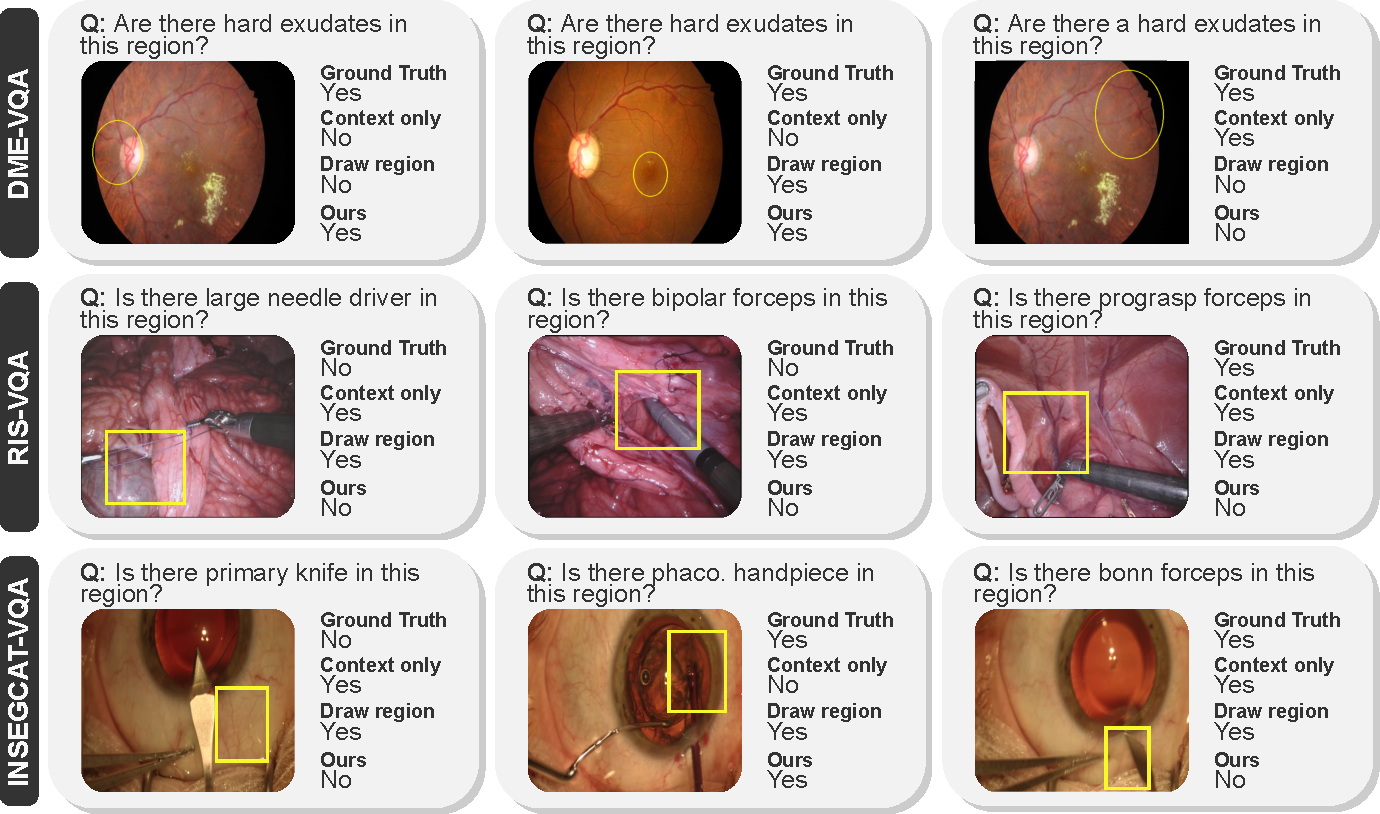
\includegraphics[width=0.90\textwidth]{Figures/Part1_LocVQA/02_llm/examples.pdf}
\caption{Qualitative examples on the DME-VQA (first row), RIS-VQA (second row), and INSEGCAT-VQA (third row) datasets. See Appendix~\ref{appendix:locvqallm} for additional examples.}
\label{fig:locvqallm_examples}
\end{center}
\end{figure}
Fig.~\ref{fig:locvqallm_errors_by_location} shows error maps by region location for the DME-VQA and INSEGCAT-VQA datasets and for the four strongest baselines. On the left side of the plot, the locations of actual positives and negatives are illustrated. For the INSEGCAT-VQA dataset, this visualization reveals a location bias that other baselines without access to the region or the context may be exploiting. Due to the nature of the images (cataract surgery) and questions, regions with positive answers tend to cluster in a specific area. This, coupled with the dissimilarity of objects mentioned in the questions, explains why a baseline like \textit{crop region} achieves relatively high performance on this dataset compared to the other two datasets (see Table~\ref{tab:locvqallm_results}). Similarly, in the case of DME-VQA, it becomes evident that the lack of context in \textit{crop region} results in lower sensitivity, highlighting the significance of context even when the isolated region should theoretically provide sufficient evidence. Fig.~\ref{fig:locvqallm_errors_by_location} also demonstrates that \textit{draw region} and \textit{context only} exhibit marked clusters of false positives and false negatives, potentially indicating the utilization of location biases. In contrast, our method produces a more evenly distributed location for both types of errors.
\begin{figure}[!b]
\begin{center}
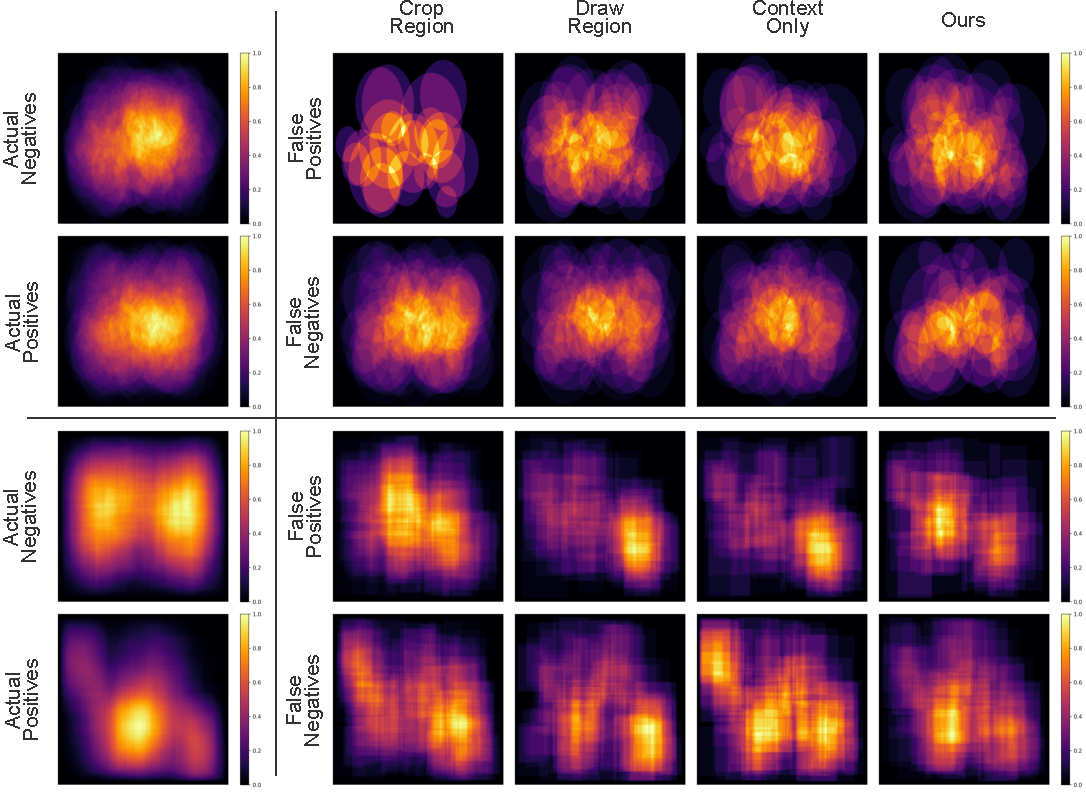
\includegraphics[width=0.85\textwidth]{Figures/Part1_LocVQA/02_llm/errors_by_location.pdf}
\caption{Error analysis by region location for the four strongest baselines. The maps are obtained by adding binary masks representing the regions for all QA pairs in each category and then normalizing. \textbf{Top:} DME-VQA dataset. \textbf{Bottom:} INSEGCAT-VQA dataset. The maps for RIS-VQA can be found in Appendix~\ref{appendix:locvqallm}.}
\label{fig:locvqallm_errors_by_location}
\end{center}
\end{figure}



\section{Conclusion}
\label{sec:locvqallm_conclusion}

In this work, we introduced a novel approach to enable localized questions in multimodal \glspl{llm} for the tasks of \gls{vqa}. Our proposed approach involves the utilization of targeted visual prompting, granting the model access not only to the region and its context within the image but also to an isolated version of the region. By doing so, we allow two perspectives to be encoded in the prompt and allow more fine-grained information to be leveraged. Our approach demonstrates enhanced performance across all evaluated datasets compared to a variety of baselines. Analysis of the results highlights how biases in the datasets can be interpreted and qualitative examples shown depict failure modes of our method. Future works include extending the methodology to accommodate multiple images and enabling the use of comparison questions.
\part{Enhancing Consistency in VQA}
\label{part:consistency}
\chapter{Consistency-preserving Visual Question Answering in Medical Imaging}
\label{chapter:cons_mainsub}
% MICCAI 2022 paper about consistency by including annotations about main and sub

Since \gls{vqa} models can be asked multiple questions about the same image, one important aspect of their behavior is what constraints there should be in the answers, given that the questions are related. This is, what level of agreement there should be in the answers so that these do not produce a contradiction. Most of the research in \gls{medvqa} has been focused on improving architectures and working with limited data, while consistency has been overlooked.  

In this work, we tackle the issue of inconsistency in \gls{medvqa} by using a novel loss function term and corresponding training strategy that allows us to consider relations between question-answer pairs in the training process. Following previous approaches from natural images, we examine the case in which the relation between reasoning and perception questions is known. We evaluate our proposed approach on the task of \gls{dme} staging from fundus images. Our experimental results show that our approach enhances not only the consistency of the model but also the overall performance.


\textbf{Author Contribution} This work was co-authored with Pablo Márquez-Neila and Raphael Sznitman. My contributions include the dataset creation, the formulation and implementation of the method, the experimental setup, result analysis and visualization, and the composition of the manuscript. 

\textbf{Publication} This work is published in the Proceedings of the MICCAI 2022 conference~\cite{tascon2022consistency}.

\newpage

% Paper contents
\section{Background and Previous Work}
\label{sec:mainsub_intro}

\gls{vqa} models are neural networks that answer natural language questions about an image by interpreting the question and the image provided~\cite{antol2015vqa,goyal2017making,hudson2019gqa,tan2019lxmert}. Specifying questions using natural language gives \gls{vqa} models great appeal, as the set of possible questions one can ask is enormous and does not need to be identical to the set of questions used to train the models. Due to these advantages, \gls{vqa} models for medical applications have also been proposed~\cite{gong2021cross,ImageCLEFVQA_Med2018,liao2020aiml,liu2019effective,vu2020question,zhan2020medical}, whereby allowing clinicians to probe the model with subtle differentiating questions and contributing to build trust in predictions.

To date, much of the work in \gls{medvqa} has focused on building more effective model architectures~\cite{gong2021cross,liao2020aiml,vu2020question} or overcoming limitations in \gls{medvqa} datasets~\cite{Nguyen19,liao2020aiml,sarrouti2020nlm,zhan2020medical}. Yet a critical component of \gls{vqa} is the notion of {\it consistency} in the answers produced by a model. Here, consistency refers to a model's capacity to produce answers that are not self-contradictory. For instance, the task of staging \gls{dme} from color fundus photograph illustrated in Fig.~\ref{fig:motivation} involves identifying {\it perception} elements in the image (\eg,~``are there hard exudates visible near the macula?'') to infer a disease stage, which can be expressed as a {\it reasoning} question (\eg,~``what is the stage of disease?''). Ultimately, for any \gls{vqa} model to be trustworthy, it should be able to answer these without contradicting itself (\ie, answer that the image is healthy, but also identify hard exudates in the periphery of the eye).
\begin{figure}[t]
\begin{center}
\includegraphics[width=0.75\textwidth]{Figures/Part2_Consist/01_mainsub/motivation_alt.pdf}
\caption{VQA inconsistency in Diabetic Macular Edema staging from fundus photograph. While the VQA model correctly answers ``Is the image healthy?" (left), it incorrectly answers yes to ``Are there hard exudates here?" for a specified retinal region (right).}
\label{fig:motivation}
\end{center}
\end{figure}

\nocite{wang2021image}

Consistency in \gls{vqa} has been been studied in the broader computer vision context~\cite{goel2021iq,gokhale2020vqa,ray2019sunny,ribeiro2019red,shah2019cycle}, where the relation between perception and reasoning questions is unconstrained. That is, the answers to perception questions do not necessarily imply any information with respect to the reasoning question and vice-versa. In these broad cases, some methods have modeled question implications \cite{ray2019sunny,ribeiro2019red} or rephrased questions~\cite{shah2019cycle} by generating tailored question-answer pairs (\eg,~consistent data-augmentation). Alternatively,~\cite{gokhale2020vqa,teney2019incorporating,yuan2021perception} used relations between questions to impose constraints in the \gls{vqa}'s embedding space. To avoid needing to know the relation between questions,~\cite{selvaraju2020squinting} proposed to enforce consistency by making attention maps of reasoning and perception questions similar to one another. 
However, even though these approaches tackle unconstrained question relations, the ensuring of \gls{vqa} models' consistency remains limited and often reduces the overall performance~\cite{selvaraju2020squinting}.  

Instead, we propose a novel approach to enforce \gls{vqa} consistency that is focused on cases where answers to the perception questions have explicit implications on reasoning question answers and vice-versa (\eg, cancerous cells and severity of cancer found in H\&E staining, or presence of hard exudates and \gls{dme} staging). By focusing on this subset of question relations, our aim is to improve both the accuracy of our model and its consistency, without needing external data as in~\cite{ribeiro2019red,Nguyen19,goel2021iq}. To do this, we allow questions to probe arbitrary image regions by masking irrelevant parts of the image and passing the masked image to the \gls{vqa} model (see Fig.~\ref{fig:motivation}). To then enforce consistency, we propose a new loss function that penalizes incorrect perceptual predictions when reasoning ones are correct for a given image. To validate the impact of our approach, we test it in the context of \gls{dme} staging and show that it outperforms state-of-the-art methods for consistency, without compromising overall performance accuracy. 
\section{Method}
\label{sec:mainsub_method}

We present here our approach, which consists of using a simple \gls{vqa} model with a training protocol that encourages consistency among pairs of perception and reasoning questions. Fig.~\ref{fig:method_mainsub} illustrates this \gls{vqa} model and our training approach.

\subsection{VQA Model} Following~\cite{cadene2019rubi}, our \gls{vqa} model,~$f:\mathcal{I}\times\mathcal{Q}\to \mathcal{P}(\mathcal{A})$, takes a tuple containing an image,~$\x$, and a question,~$\q$, to produce a distribution,~$\p=f(\x,\q)$, over a finite set of possible answers~$\mathcal{A}$ (see Fig.~\ref{fig:method_mainsub}(Top)). After encoding the inputs, the \gls{vqa} model combines visual ($v$) and textual ($q$) features through an attention module ($k$)~\cite{xu2015show} that selects the visual features relevant to the question ($v'$). The final classifier receives a combination of the relevant features and the text features through a fusion module to predict the final distribution.

In some cases, questions may be asking about content related to specific regions of the image (\eg, ``are there hard exudates in this region?''). To process these cases, the input image is masked so that the visible area corresponds to the region mentioned in the question while the rest of the image is set to zero.

Training this model requires a dataset~$\mathcal{T}=\{t^{(i)}=(\x^{(i)}, \q^{(i)}, a^{(i)})\}_{i=1}^N\subseteq\mathcal{I}\times\mathcal{Q}\times\mathcal{A}$ of images and questions annotated with their answers. The \gls{vqa}~loss is simply the cross-entropy between the predicted distribution and the real answer,
\begin{equation}
    \label{eq:vqa_loss}
    \ell_{\textrm{VQA}}(\p, a) = H(\p, a) = -\log \p_a.
\end{equation}
While this loss alone is sufficient to reach a reasonable performance, it ignores the potentially useful interactions that may exist among training questions.
\begin{figure}[!h]
\begin{center}
\includegraphics[width=0.75\textwidth]{Figures/Part2_Consist/01_mainsub/method.pdf}
\caption{\textbf{Top:} VQA model architecture. \textbf{Bottom:} Visualization of the training process with the proposed loss. The total loss, $\ell_{\textrm{tot}}$, is based on two terms: the conventional VQA loss,  $\ell_{\textrm{VQA}}$ and our proposed consistency loss term, $\ell_{\textrm{cons}}$. The latter is computed only for pairs of main (reasoning) and sub (perception) questions. Training mini-batches consist of main and sub-questions at the same time, whereby sub-questions can consider specific regions of the image. Unrelated questions (denoted with ``ind") can also be included in training batches but do not contribute to $\ell_{\textrm{cons}}$.}
\label{fig:method_mainsub}
\end{center}
\end{figure}


\subsection{Consistency Loss} We aim to improve the quality of our \gls{vqa} model by exploiting the relationships between reasoning and perception questions at training time. To this end, we augment the training dataset with an additional binary relation~$\prec$ over the set of questions~$\mathcal{Q}$. Two questions are related, $\q^{(i)}\prec \q^{(j)}$, if $\q^{(i)}$ is a perception question associated to the reasoning question~$\q^{(j)}$. From hence on, we refer to perception questions as \emph{sub-questions} and reasoning questions as \emph{main questions}.

Following the terminology in~\cite{selvaraju2020squinting}, an inconsistency occurs when the \gls{vqa} model infers the main question correctly but the sub-question incorrectly. Using the entropy as a measurement of incorrectness, we propose to impose the consistency at training time by penalizing the cases with high $H^{(i)}=H(\p^{(i)}, a^{(i)})$ and low $H^{(j)}=H(\p^{(j)}, a^{(j)})$ when $\q^{(i)}\prec \q^{(j)}$. To do this, we use an adapted hinge loss that disables the penalty when $H^{(j)}$ is larger than a threshold~$\gamma>0$, but otherwise penalizes large values of~$H^{(i)}$,
\begin{equation}
    \label{eq:cons_loss}
    \ell_{\textrm{cons}}(H^{(i)}, H^{(j)}) = H^{(i)}\max\{0, \gamma - H^{(j)}\}.
\end{equation}
\noindent
%$\gamma \in \mathbb{R}^+$. Fig.~\ref{fig:method_mainsub}(Bottom) illustrates $\ell_{\textrm{cons}}$. 

The final cost function then minimizes the expected value of the \gls{vqa} loss~\eqref{eq:vqa_loss} for the elements of the training dataset and the consistency loss~\eqref{eq:cons_loss} for the pairs of training samples with $\prec$-related questions,
\begin{equation}
    \label{eq:cost}
    \mathbb{E}_{t\sim\mathcal{T}}[\ell_\textrm{VQA}(\p, a)] +
    \lambda\mathbb{E}_{(t^{(i)}, t^{(j)})\sim\mathcal{T}^2}[\ell_\textrm{cons}(H^{(i)}, H^{(j)}) \mid \x^{(i)}=\x^{(j)}, \q^{(i)}\prec\q^{(j)}],
\end{equation}
where $\lambda > 0$ controls the relative strength of both losses and $\mathcal{T}^2$ is the Cartesian product of $\mathcal{T}$ with itself, that is, all pairs of training samples.

To train, this cost is iteratively minimized approximating the expectations with mini-batches. The two expectations of Eq.~\eqref{eq:cost} suggest that two mini-batches are necessary at each iteration: one mini-batch sampled from~$\mathcal{T}$ and a second mini-batch of $\prec$-related pairs sampled from $\mathcal{T}^2$. However, in practice a single mini-batch is sufficient as long as we ensure that it contains pairs of $\prec$-related questions. While this biased sampling could in turn bias the estimation of the first expectation, we did not observe a noticeable impact in our experiments. Fig.~\ref{fig:method_mainsub}(Bottom) illustrates this training procedure.
\section{Experiments and Results}

\subsection{DME Staging}
\gls{dme} staging from color fundus images involves grading images on a scale from 0 to 2, with 0 being healthy and 2 being severe (see Fig.~\ref{fig:dme}). Differentiation between the grades relies on the presence of hard exudates present in different locations of the retina. Specifically, a grade of 0 implies that no hard exudates are present at all, a grade of 1 implies that hard exudates are located in the retina periphery (\ie,~outside a circular region centered at the fovea center with radius of one optic disc diameter), and a grade of 2 when hard exudates are in the macular region~\cite{ren2018diabetic}.
\begin{figure}[b!]
\begin{center}
\includegraphics[width=0.9\textwidth]{Figures/Part2_Consist/01_mainsub/dme_2.pdf}
\caption{DME risk grading. Grade 0 is assigned if there are no hard exudates present in the whole image. Grade 1 is assigned if there are hard exudates, but only located outside a circle centered at the fovea with radius of one optic disc diameter. Grade 2 is assigned if there are hard exudates located within the circle. Examples of main and sub-questions are provided for each grade.}
\label{fig:dme}
\end{center}
\end{figure}

\subsection{Dataset}
To validate our method, we make use of two publicly available datasets: the Indian Diabetic Retinopathy Image Dataset (IDRiD)~\cite{idrid} and the e-Ophta dataset~\cite{decenciere2013teleophta}. From the IDRiD dataset, we use images from the segmentation and grading tasks, which consist of 81 and 516 images, respectively. Images from the segmentation task include segmentation masks for hard exudates and images from the grading task only have the \gls{dme} grade. On the other hand, the e-Ophta dataset comprises 47 images with segmentation of hard exudates and 35 images without lesions. Combining both datasets yields a dataset of 128 images with segmentation masks for hard exudates and 128 images without any lesions, plus 423 images for which only the \gls{dme} risk grade is available. 

In this context, we consider main questions to be those asking ``What is the \gls{dme} risk grade?" when considering the entire image. Sub-questions were then defined as questions asking about the presence of the hard exudates. For instance, as shown in Fig.~\ref{fig:dme}{(Right)}, ``Are there hard exudates in this region?" where the region designated contains the macula. In practice, we set three types of sub-questions: ``are there hard exudates in this image?", ``are there hard exudates in the macula?" and ``are there hard exudates in this region?". We refer to these three questions as \textit{whole}, \textit{macula} and \textit{region} questions, respectively. For the region sub-questions, we consider circular regions that can be centered anywhere, or centered on the fovea, depending on availability of fovea center location annotations. As mentioned in Sec.~\ref{sec:mainsub_method}, to answer questions about regions, images are masked so that only the region is visible.

The total number of question-answer pairs in our dataset consists of 9779 for training {(4.4\% main, 21.4\% sub, 74.2\% ind)}, 2380 for validation {(4.5\% main, 19.2\% sub, 76.3\% ind)} and 1311 for testing {(10\% main, 46.1\% sub, 43.9\% ind)}, with images in the train, validation and test sets being mutually exclusive.

\subsection{Experimental Setup}

We compare our approach to a baseline model that does not use the proposed $\ell_{\textrm{cons}}$ loss, equivalent to setting $\lambda=0$. In addition, we compare our method against the attention-matching method, SQuINT~\cite{selvaraju2020squinting}, as it is a state-of-the-art alternative to our approach that can be used with the same \gls{vqa} model architecture.

Our \gls{vqa} model uses an ImageNet-pretrained ResNet101~\cite{he2016deep} with input image of $448\times 448$~pixels and an embedding of 2048~dimensions for the image encoding. For text encoding, a single-layer \gls{lstm}~\cite{hochreiter1997long} network processes the input question with word encoding of length 300 and produces a single question embedding of 1024~dimensions. The multi-glimpse attention mechanism~\cite{xu2015show} uses 2~glimpses and dropout rate~$0.25$, and the multimodal fusion stage uses standard concatenation. The final classifier is a multi-layer perceptron with hidden layer of 1024 dimensions and dropout rate of 0.25. Hyperparameters~$\lambda$ and~$\gamma$ were empirically adjusted to 0.5 and~1.0, respectively. 

All experiments were implemented using PyTorch~1.10.1 and run on a Linux machine with an NVIDIA RTX 3090 graphic card using 16~GB of memory and 4~CPU cores. All methods use the weighted cross-entropy as the base \gls{vqa} loss function. Batch size was set to~64, and we used Adam for optimization with a learning rate of $10^{-4}$. Maximum epoch number was 100 and we use early stopping policy to prevent overfitting, with patience of 20~epochs \footnote{Our code and data are available at \url{https://github.com/sergiotasconmorales/consistency_vqa}}.

We report accuracy and consistency~\cite{selvaraju2020squinting} performances, using two different definitions of consistency for comparison. Consistency, C1, is the percentage of sub-questions that are answered correctly when the main question was answered correctly. Consistency, C2, is the percentage of main questions that are answered correctly when all corresponding sub-questions were answered correctly.

\subsection{Results}
Table \ref{tab:results} shows the results.
% for the best values of the hyperparameters $\lambda$ and $\gamma$. \RS{I don't understand this. Do we have other values of $\lambda$ and $\gamma$. Do we have that as well for Squint}.
We compare these results to the case in which the value of $\lambda$ is~0, which corresponds to the baseline in which no additional loss term is used. For each case, we present the overall accuracy and the accuracy for each type of question, as well as the consistency values. Fig.~\ref{fig:examples} illustrates the performance of each method with representative qualitative examples.


\begin{table}[!t]
\begin{center}
\resizebox{\textwidth}{!}{
\begin{tabular}{llllllll}
\toprule
\multicolumn{1}{l}{\multirow{2}{*}{Case}}    &  \multicolumn{5}{c}{Accuracy} & \multicolumn{2}{c}{Consistency} \\ \cline{2-8} \multicolumn{1}{c}{}  
                   & \multicolumn{1}{l}{overall}      & \multicolumn{1}{l}{grade}        & \multicolumn{1}{l}{whole}        & \multicolumn{1}{l}{macula}       & \multicolumn{1}{l}{region}       & \multicolumn{1}{c}{C1}            & \multicolumn{1}{c}{C2}          

\\ \hline
\multicolumn{1}{l}{Baseline (no att.)}                                 & \multicolumn{1}{l}{77.54 } & \multicolumn{1}{l}{73.59} & \multicolumn{1}{l}{81.37 } & \multicolumn{1}{l}{83.37}& \multicolumn{1}{l}{76.66 } & \multicolumn{1}{l}{81.70 }  & \multicolumn{1}{l}{91.86 } 

\\ 
\multicolumn{1}{l}{Baseline (att.)}                            & \multicolumn{1}{l}{81.46 } & \multicolumn{1}{l}{80.23} & \multicolumn{1}{l}{83.13 } & \multicolumn{1}{l}{\textbf{87.18} }& \multicolumn{1}{l}{80.58 } & \multicolumn{1}{l}{89.21 }  & \multicolumn{1}{l}{96.92 } 

\\ 
\multicolumn{1}{l}{Baseline (att.) + SQuINT~\cite{selvaraju2020squinting}  }                                  & \multicolumn{1}{l}{80.58} & \multicolumn{1}{l}{77.48} & \multicolumn{1}{l}{82.82} & \multicolumn{1}{l}{85.34}& \multicolumn{1}{l}{80.02} & \multicolumn{1}{l}{88.17}  & \multicolumn{1}{l}{94.62} 

\\ 
\multicolumn{1}{l}{Baseline (att.) + Ours ($\lambda=0.5,\gamma=1$)}             & \multicolumn{1}{l}{\textbf{83.49} } & \multicolumn{1}{l}{\textbf{80.69} } & \multicolumn{1}{l}{\textbf{84.96} } & \multicolumn{1}{l}{\textbf{87.18} } & \multicolumn{1}{l}{\textbf{83.16}} & \multicolumn{1}{l}{\textbf{94.20} } & \multicolumn{1}{l}{\textbf{98.12} } 

\\ \bottomrule                  
\end{tabular}
}
\end{center}
\caption{Average test accuracy and consistency values for the different models. Results shown are averaged over 10 models trained with different seeds. Accuracy values are presented for all questions (overall), for main questions (grade) and for sub-questions (whole, macula and region). Both measures of consistency are shown as well.}
\label{tab:results}
\end{table}
\begin{figure}[!t]
\begin{center}
\includegraphics[width=0.99\textwidth]{Figures/Part2_Consist/01_mainsub/examples_expl_marked_add.pdf}
\caption{Qualitative examples from the test set. Inconsistent sub-answers are highlighted in red. Additional examples are shown in Appendix~\ref{appendix:consistency_mainsub}.  
}
\label{fig:examples}
\end{center}
\end{figure}


\begin{table}[!t]
\begin{center}
\begingroup
\setlength{\tabcolsep}{10pt} % Default value: 6pt
\renewcommand{\arraystretch}{1.5} % Default value: 1
\begin{tabular}{lllllllll}
\toprule
 \multicolumn{1}{c}{\multirow{2}{*}{$\lambda$}} & \multicolumn{1}{c}{\multirow{2}{*}{$\gamma$}} & \multicolumn{5}{c}{Accuracy}   & \multicolumn{2}{c}{Consistency}  \\ \cline{3-9} 
\multicolumn{1}{c}{}                         & \multicolumn{1}{c}{}      &  \multicolumn{1}{c}{overall}                       & \multicolumn{1}{c}{grade}      & \multicolumn{1}{c}{whole}        & \multicolumn{1}{c}{macula}        & \multicolumn{1}{c}{region}     & \multicolumn{1}{c}{C1}            & \multicolumn{1}{c}{C2}          
\\ \hline

\multicolumn{1}{l}{0}                     & \multicolumn{1}{l}{-}                    & \multicolumn{1}{l}{81.46} & \multicolumn{1}{l}{80.23} & \multicolumn{1}{l}{83.13} & \multicolumn{1}{l}{87.18} & \multicolumn{1}{l}{80.58} & \multicolumn{1}{l}{89.21} & \multicolumn{1}{l}{96.92} 

\\ \hline 

\multicolumn{1}{l}{0.2}                     & \multicolumn{1}{l}{0.5}                    & \multicolumn{1}{l}{82.01} & \multicolumn{1}{l}{80.38} & \multicolumn{1}{l}{83.59} & \multicolumn{1}{l}{86.56} & \multicolumn{1}{l}{81.36} & \multicolumn{1}{l}{90.93} & \multicolumn{1}{l}{97.38} 

\\ 
\multicolumn{1}{l}{0.2}                     & \multicolumn{1}{l}{1}                    & \multicolumn{1}{l}{82.65} & \multicolumn{1}{l}{ 79.77} & \multicolumn{1}{l}{ 83.97} & \multicolumn{1}{l}{ 86.64} & \multicolumn{1}{l}{82.30} & \multicolumn{1}{l}{ 93.22} & \multicolumn{1}{l}{97.51 } 

\\ 

\multicolumn{1}{l}{0.2}                     & \multicolumn{1}{l}{1.5}                    & \multicolumn{1}{l}{83.05} & \multicolumn{1}{l}{81.22} & \multicolumn{1}{l}{ 84.27} & \multicolumn{1}{l}{ 87.33} & \multicolumn{1}{l}{82.53} & \multicolumn{1}{l}{ 93.23} & \multicolumn{1}{l}{ 97.56} 


\\ \hline 
\multicolumn{1}{l}{0.3}                     & \multicolumn{1}{l}{0.5}                   & \multicolumn{1}{l}{82.34} & \multicolumn{1}{l}{ 79.92} & \multicolumn{1}{l}{ 83.59} & \multicolumn{1}{l}{ 87.71} & \multicolumn{1}{l}{81.74} & \multicolumn{1}{l}{ 92.32} & \multicolumn{1}{l}{ 97.31} 

\\ 

\multicolumn{1}{l}{0.3}                     & \multicolumn{1}{l}{1}                 & \multicolumn{1}{l}{83.27} & \multicolumn{1}{l}{ 80.53} & \multicolumn{1}{l}{ 84.58} & \multicolumn{1}{l}{ 87.25} & \multicolumn{1}{l}{82.91} & \multicolumn{1}{l}{ 94.01} & \multicolumn{1}{l}{ 98.10} 

\\ 

\multicolumn{1}{l}{0.3}                     & \multicolumn{1}{l}{1.5}                   & \multicolumn{1}{l}{83.28} & \multicolumn{1}{l}{80.84 } & \multicolumn{1}{l}{ 84.43} & \multicolumn{1}{l}{ 87.48} & \multicolumn{1}{l}{82.86} & \multicolumn{1}{l}{ 93.28} & \multicolumn{1}{l}{ 98.29} 


\\ \hline 

\multicolumn{1}{l}{0.4}                     & \multicolumn{1}{l}{0.5}                   & \multicolumn{1}{l}{82.87} & \multicolumn{1}{l}{80.69} & \multicolumn{1}{l}{ 84.89} & \multicolumn{1}{l}{ 87.02} & \multicolumn{1}{l}{82.30} & \multicolumn{1}{l}{ 92.66} & \multicolumn{1}{l}{ 96.66} 

\\ 
\multicolumn{1}{l}{0.4}                     & \multicolumn{1}{l}{1}                 & \multicolumn{1}{l}{82.97} & \multicolumn{1}{l}{ 80.15} & \multicolumn{1}{l}{ 83.97} & \multicolumn{1}{l}{ 86.72} & \multicolumn{1}{l}{82.69} & \multicolumn{1}{l}{ 93.91} & \multicolumn{1}{l}{98.23} 

\\ 
\multicolumn{1}{l}{0.4}                     & \multicolumn{1}{l}{1.5}                  & \multicolumn{1}{l}{83.33} & \multicolumn{1}{l}{ 80.08} & \multicolumn{1}{l}{ 84.20} & \multicolumn{1}{l}{ 86.87} & \multicolumn{1}{l}{83.17} & \multicolumn{1}{l}{ 93.96} & \multicolumn{1}{l}{ 97.77} 

\\ \hline 
\multicolumn{1}{l}{0.5}                     & \multicolumn{1}{l}{0.5}                & \multicolumn{1}{l}{82.54} & \multicolumn{1}{l}{81.07 } & \multicolumn{1}{l}{ 83.66} & \multicolumn{1}{l}{ 88.02} & \multicolumn{1}{l}{81.81} & \multicolumn{1}{l}{ 91.87} & \multicolumn{1}{l}{ 97.73} 

\\ 
\multicolumn{1}{l}{0.5}                     & \multicolumn{1}{l}{1}                    & \multicolumn{1}{l}{83.49} & \multicolumn{1}{l}{80.69 } & \multicolumn{1}{l}{84.96 } & \multicolumn{1}{l}{87.18} & \multicolumn{1}{l}{83.16} & \multicolumn{1}{l}{94.20} & \multicolumn{1}{l}{98.12 } 

\\ 
\multicolumn{1}{l}{0.5}                     & \multicolumn{1}{l}{1.5}             & \multicolumn{1}{l}{83.25} & \multicolumn{1}{l}{ 79.92} & \multicolumn{1}{l}{ 84.58} & \multicolumn{1}{l}{ 86.95} & \multicolumn{1}{l}{83.01} & \multicolumn{1}{l}{ 94.20} & \multicolumn{1}{l}{ 98.12} 

\\ \bottomrule                  
\end{tabular}
\endgroup
\end{center}
\caption{Average test accuracy and consistency values for different values of the parameters $\lambda$ and $\gamma$. The first row ($\lambda\, =\, 0$) corresponds to no consistency enhancement method.}
\label{tab:results_params}
\end{table}
In general, we observe that our proposed approach yields increases in accuracy and consistency when compared to both the baseline and SQuINT. Importantly, this increase in consistency is not at the expense of overall accuracy. Specifically, this indicates that our loss term causes the model to be correct about sub-questions when it is correct about main questions. The observed increase in accuracy also indicates that our approach is not synthetically increasing consistency by reducing the number of correct answers on main questions~\cite{selvaraju2020squinting}. We note that SQuINT results in a reduction in accuracy and consistency, which can be partially explained by the presence of region questions that are not associated to any main question. These questions, which exceed the number of main questions, may affect the constraint in the learned attention maps.

Table~\ref{tab:results_params} shows the effect of $\lambda$ and $\gamma$ on the performance metrics. As expected, we notice that when $\lambda$ increases, the consistency of our approach increases as well and will occasionally deteriorate overall accuracy. The impact of $\gamma$ however is less evident, as no clear trend is visible. This would imply that the exact parameter value used is moderately critical to performances. 
\section{Conclusion}

In this work, we presented a novel method for improving consistency in \gls{vqa} models in cases where answers to sub-questions imply those of main questions and vice-versa. By using a tailored training procedure and loss function that measures the level of inconsistency, we show on the application of \gls{dme} staging, that our approach provides important improvements in both \gls{vqa} accuracy and consistency. In addition, we show that our method's hyperparameters are relatively insensitive to model performance. In the future, we plan to investigate how this approach can be extended to the broader case of unconstrained question relations.
\chapter{Logical Implications for Visual Question Answering Consistency}
\label{chapter:cons_logic}
% CVPR 2023 paper about consistency through logical relations

The previous chapter presented a method to encourage a \gls{vqa} method to be more consistent by considering pairs of reasoning and perception questions and their relationship. While this consideration is useful for imposing a more consistent behavior, the relation of main and sub (or reasoning and perception) between QA pairs requires assumptions about the nature of the questions. We observe that a more general definition of consistency is required, and explore, from the perspective of logic, the possible relations that can exist between the propositions that the QA pairs represent. 

The present work presents a more general framework for consistency enforcement and assessment. We make use of concepts from logic in order to establish a more robust definition of inconsistency. Then, we encourage the model to provide more consistent answers by integrating annotations about logical relations between pairs of propositions into the training process. Since these annotations are not commonly included in \gls{vqa} datasets, we propose an auxiliary method to predict them. We evaluate our method on multiple architectures and across different datasets with both natural and medical images, showing that our consistency framework improves the overall performance of the model while reducing inconsistencies.

\textbf{Author Contribution} The co-authors of this work are Pablo Márquez-Neila and Raphael Sznitman. My contributions are as follows: Data annotation, dataset creation, methodology and implementation thereof, experimental design, result analysis, and visualization, as well as the writing of the manuscript.

\textbf{Publication} This work is published in the Proceedings of the CVPR 2023 conference~\cite{tascon2023logical}.

\newpage

% Paper contents
\section{Background and previous work}

\subsection{Background}
\gls{vqa} models have drawn recent interest in the computer vision community as they allow text queries to question image content. This has given way to a number of novel applications in the space of model reasoning~\cite{wang2015explicit,cadene2019murel,wu2021multi,jing2022maintaining}, medical diagnosis~\cite{nguyen2019overcoming,vu2020question,gupta2021hierarchical,zhan2020medical} and counterfactual learning~\cite{agarwal2020towards,chen2020counterfactual,abbasnejad2020counterfactual}. With the ability to combine language and image information in a common model, it is unsurprising to see a growing use of \gls{vqa} methods.

Despite this recent progress, however, a number of important challenges remain when making \gls{vqa}s more proficient. For one, it remains extremely challenging to build \gls{vqa} datasets that are void of bias. Yet this is critical to ensure subsequent models are not learning spurious correlations or shortcuts~\cite{teney2020unshuffling}. This is particularly daunting in applications where domain knowledge plays an important role (\eg,  medicine~\cite{he2020pathvqa,lau2018dataset,do2021multiple}). Alternatively, ensuring that responses of a \gls{vqa} are coherent, or {\it consistent}, is paramount as well. That is, \gls{vqa} models that answer differently about similar content in a given image imply inconsistencies in how the model interprets the inputs. A number of recent methods have attempted to address this using logic-based approaches~\cite{gokhale2020vqa}, rephrashing~\cite{shah2019cycle}, question generation~\cite{ribeiro2019red,ray2019sunny, goel2021iq} and regularizing using consistency constraints~\cite{tascon2022consistency}. In this work, we follow this line of research and look to yield more reliable \gls{vqa} models.

\begin{figure}[!b]
\centering
\includegraphics[width=0.6\textwidth]{Figures/Part2_Consist/02_logic/image_intro.pdf}
\caption{\textbf{Top:} Conventional VQA models tend to produce inconsistent answers as a consequence of not considering the relations between question and answer pairs. \textbf{Bottom:} Our method learns the logical relation between question and answer pairs to improve consistency.
} 
\label{fig:image_intro}
\end{figure}

We wish to ensure that \gls{vqa} models are consistent in answering questions about images. This implies that if multiple questions are asked about the same image, the model's answers should not contradict themselves. For instance, if one question about the image in \fig~\ref{fig:image_intro} asks ``Is there snow on the ground?", then the answer inferred should be consistent with that of the question ``Is it the middle of summer?" As noted in~\cite{selvaraju2020squinting}, such question pairs involve reasoning and perception, and consequentially lead the authors to define inconsistency when the reasoning and perception questions are answered correctly and incorrectly, respectively. Along this line,~\cite{tascon2022consistency} uses a similar definition of inconsistency to regularize a \gls{vqa} model meant to answer medical diagnosis questions that are hierarchical in nature. What is critical in both cases, however, is that the consistency of the \gls{vqa} model depends explicitly on its answers, as well as the question and true answer. This hinges on the assumption that perception questions are sufficient to answer reasoning questions. Yet, for any question pair, this may not be the case. As such, the current definition of consistency (or inconsistency) has been highly limited and does not truly reflect how \gls{vqa}s should behave. 

To address the need to have self-consistent \gls{vqa} models, we propose a novel training strategy that relies on logical relations. To do so, we re-frame question-answer (QA) pairs as propositions and consider the relational construct between pairs of propositions. This construct allows us to properly categorize pairs of propositions in terms of their logical relations. From this, we introduce a novel loss function that explicitly leverages the logical relations between pairs of questions and answers in order to enforce that \gls{vqa} models be self-consistent. However, datasets typically do not contain relational information about QA pairs, and collecting this would be extremely laborious and difficult. To overcome this, we propose to train a dedicated language model that infers logical relations between propositions.
Our experiments show that we can effectively infer logical relations from propositions and use them in our loss function to train \gls{vqa} models that improve state-of-the-art methods via consistency. We demonstrate this over two different \gls{vqa} datasets, against different consistency methods, and with different \gls{vqa} model architectures.

\subsection{Previous Work}
Since its initial presentation in Antol et al.~\cite{antol2015vqa}, \gls{vqa} has thoroughly advanced. Initial developments focused on multimodal fusion modules, which combine visual and text embeddings~\cite{nam2017dual,cadene2019murel}. From basic concatenation and summation~\cite{antol2015vqa} to more complex fusion mechanisms that benefit from projecting the embeddings to different spaces, numerous approaches have been proposed~\cite{fukui2016multimodal,kim2016hadamard,ben2017mutan}. The addition of attention mechanisms~\cite{kim2018bilinear, nam2017dual,cadene2019murel} and subsequently transformer architectures~\cite{vaswani2017attention} has also contributed to the creation of transformer-based \gls{vlm}, such as LXMERT, which have shown state-of-the-art performances~\cite{tan2019lxmert}. 

More recently, methods have proposed to improve other aspects of \gls{vqa}, including avoiding shortcut learning and biases~\cite{dancette2021beyond,han2021greedy}, improving 3D spatial reasoning~\cite{banerjee2021weakly}, Out-Of-Distribution (OOD) generalization~\cite{cao2021linguistically,teney2020unshuffling}, improving transformer-based vision-language models~\cite{yang2021auto,zhou2021trar}, external knowledge integration~\cite{ding2022mukea,gao2022transform} and model evaluation with visual and/or textual perturbations~\cite{gupta2022swapmix,walmer2022dual}. With the awareness of bias in \gls{vqa} training data, some works have also addressed building better datasets (\eg, VQAv2.0~\cite{goyal2017making}, VQA-CP~\cite{agrawal2018don}, CLEVR~\cite{johnson2017clevr} and GCP~\cite{hudson2019gqa}).

Furthermore, these developments have now given rise to \gls{vqa} methods in specific domains. For instance, the VizWiz challenge~\cite{gurari2018vizwiz,gurari2019vizwiz,chen2022grounding} aims at creating \gls{vqa} models that can help visually impaired persons with routine daily tasks, while there is a growing number of \gls{medvqa} works with direct medicine applications~\cite{nguyen2019overcoming,gupta2021hierarchical,vu2020question,zhan2020medical}. 

\subsubsection{Consistency in VQA} Consistency in \gls{vqa} can be defined as the ability of a model to produce answers that are not contradictory. This is, given a pair of questions about an image, the answers predicted by a \gls{vqa} model should not be contrary (\eg answering ``Yes" to ``Is it the middle of summer?" and ``Winter" to ``What season is it?"). Due to its significance in reasoning, consistency in \gls{vqa} has become a focus of study in recent years~\cite{ribeiro2019red,shah2019cycle,gokhale2020vqa,selvaraju2020squinting,jing2022maintaining}. Some of the first approaches for consistency enhancement focused on creating re-phrasings of questions, either by dataset design or at training time~\cite{shah2019cycle}. Along this line, entailed questions were proposed~\cite{ribeiro2019red,gokhale2020vqa}, such that a question generation module was integrated into a \gls{vqa} model~\cite{ray2019sunny,goel2021iq}, used as a benchmarking method to evaluate consistency~\cite{yuan2021perception} or as a rule-based data-augmentation technique~\cite{ribeiro2019red}. Other approaches tried to shape the embedding space by imposing constraints in the learned representations~\cite{teney2019incorporating} and by imposing similarities between the attention maps of pairs of questions~\cite{selvaraju2020squinting}. Another work~\cite{tascon2022consistency} assumed entailment relations between pairs of questions to regularize training. A more recent approach attempts to improve consistency by using graph neural networks to simulate a dialog in the learning process~\cite{jing2022maintaining}. 

While these approaches show benefits in some cases, they typically only consider that a subset of logical relationships exists between pairs of question-answers or assume that a single relation holds for all QA pairs. Though true in the case of re-phrasings, other question generation approaches cannot guarantee that the produced questions preserve unique relations or that grammatical structure remains valid. Consequently, these methods often rely on metrics that either over or under-estimate consistency by relying on these assumptions. In the present work, we propose a strategy to alleviate these limitations by considering all logical relations between pairs of questions and answers. 

\subsubsection{Entailment Prediction} \glsxtrfull{nli}, or \gls{rte}, is the task of predicting how two input sentences (namely \textit{premise} and \textit{hypothesis}) are related, according to three pre-established categories: entailment, contradiction and neutrality~\cite{maccartney2008modeling}. For example, if the premise is ``A soccer game with multiple males playing" and the hypothesis is ``Some men are playing a sport," then the predicted relation should be an entailment, because the hypothesis logically follows from the premise. Several benchmarking datasets (\eg, SNLI~\cite{young2014image}, MultiNLI~\cite{williams2017broad}, SuperGLUE~\cite{wang2019superglue}, WIKI-FACTCHECK~\cite{sathe2020automated} and ANLI~\cite{nie2019adversarial}) have contributed to the adaption of general-purpose transformer-based models like \gls{bert}~\cite{devlin2018bert}, RoBERTa~\cite{liu2019roberta} and DeBERTa~\cite{he2020deberta} for this task. In this work, we will leverage these recent developments to build a model capable of inferring relations between propositions.
\section{Method}


\label{sec:method}
Given an image $\x \in \mathcal{I}$, a question $\q \in \mathcal{Q}$ about the image and a set $\mathcal{A}=\{a_1,\ldots, a _K\}$ of possible answers to choose from, a \gls{vqa} model is expected to infer the answer $\hat{a} \in \mathcal{A}$ that matches the true answer $a^*$. This can be formulated as, 
\begin{equation}
    \hat{a} = \argmax_{a \in \mathcal{A}} p(a | \x,\q; \bm{\theta}),
    \label{eq:vqa}
\end{equation}
where $\bm{\theta}$ represents the parameters of the \gls{vqa} model.

% In this context, consider the relation between two QA pairs $(\q _i, a_i)$ and $(\q_j, a_j)$ for the same image $\x$ -- for example, the pairs (``Is the horse brown?", ``No") and (``What is the color of the horse?", ``White"). In this case the first pair is a necessary condition for the second one or, equivalently, the second pair is a sufficient condition for the first one.

In this context, we observe that two QA pairs $(\q _i, a_i)$ and~$(\q_j, a_j)$ for the same image~$\x$ can have different kinds of logical relations. In the simplest case, the two pairs may be unrelated, as with the pairs (``Is it nighttime?'', ``Yes'') and (``Is there a bench in the image?'', ``No''). Knowing that one of the pairs is true gives no information about the truth value of the other. 

On the other hand, two pairs may be related by a logical implication, as in the pairs (``Is the horse brown?", ``No") and (``What is the color of the horse?", ``White"). Knowing that the second pair is true implies that the first pair must be true as well. Conversely, if the first pair is false (\emph{the horse is brown}), it implies that the second pair must also be false. In this case, the first pair is a necessary condition for the second one or, equivalently, the second pair is a sufficient condition for the first one. 

Finally, it can be that two QA pairs are related by a double logical implication, as with the pairs (``Is this a vegetarian pizza?'', ``Yes'') and (``Does the pizza have meat on it?'', ``No''). The veracity of the former implies the veracity of the latter, but the veracity of the latter also implies the veracity of the former. In this case, each pair is simultaneously a necessary and sufficient condition for the other pair, and both pairs are then equivalent. 

Note that the logical implication existing between two QA pairs is an intrinsic property of the QA pairs, and does not depend on the correctness of the predictions coming from a \gls{vqa} model. If a \gls{vqa} model considers a sufficient condition true and a necessary condition false, it is incurring an \emph{inconsistency} regardless of the correctness of its predictions.
% When discussing logical implications, we will only care about the truth values of the QA pairs, but not whether the VQA model

Since logical implications are the basis of reasoning, we propose to explicitly use them when training a \gls{vqa} model to reduce its inconsistent predictions.
% If we now consider any potential pair of QAs, then four possible {logical interactions} could be observed: (1) sufficient, (2) necessary, (3) equivalent or (4) unrelated. Since these types of relationships are the basis of reasoning, we propose to explicitly use them when training a VQA model to reduce its inconsistent predictions.
Unfortunately, doing so requires overcoming two important challenges: (1)~a strategy is needed to train \gls{vqa} models with logical relations that leverage consistency in a purposeful manner. Until now, no such approach has been proposed; (2)~\gls{vqa} datasets do not typically contain logical relations between pairs of QA. Acquiring these manually would, however, be both time-consuming and difficult.

We address these challenges in this work by formalizing the idea of consistency and treating QA pairs as logical propositions from which relations can comprehensively be defined. Using this formalism, we first propose a strategy to solve (1) and train a \gls{vqa} model more effectively using logical relations and the consistency they provide~(Sec.~\ref{subsec:loss}). We then show in Sec.~\ref{subsec:relation_prediction} how we infer relations between pairs of propositions, thereby allowing standard \gls{vqa} datasets to be augmented with logical relations.

%%----------------------------$$

%\begin{figure*}[!t]
%\centering
%\includegraphics[width=0.85\textwidth]{images/method.pdf}
%\caption{Overview of our method. The VQA model receives a batch of images and questions that has been sampled so that related questions are consecutive. The scores provided by the model are used to compute a common VQA loss $\ell_{\textrm{VQA}}$, as well as the proposed consistency loss $\ell_{\textrm{cons}}$. For the latter, the logical implications between the pairs of question-answers are considered so as to avoid inconsistent cases.}
%\label{fig:method}
%\end{figure*}


\subsection{Consistency Formulation}
\label{subsec:consistency_framework}

We begin by observing that QA pairs~$(\q, a)$ can be considered and treated as logical propositions.
For instance, the QA (``Is it winter?", ``Yes") can be converted to ``It is winter," which is a logical proposition that can be evaluated as \emph{true} or \emph{false} (\ie,~its \emph{truth value}). Doing so allows us to use a broad definition of consistency, namely one that establishes that two propositions are inconsistent if both cannot be true at the same time~\cite{bradley1979possible}. In the context of this work, we assume the truth value of a proposition~$(\q, a)$ is determined by an agent (either a human annotator or the \gls{vqa} model) after observing the information contained in an image~$\x$. 

Let $\mathcal{D} = \mathcal{I}\times \mathcal{Q} \times \mathcal{A}$ be a \gls{vqa} dataset that contains triplets $(\x^{(n)}, \q_i^{(n)}, a_i^{(n)})$, where $\x^{(n)}$ is the $n$-th image and $(\q_i^{(n)}, a_i^{(n)})$ is the $i$-th question-answer pair about $\x^{(n)}$. In the following, we omit the index~$n$ for succinctness. For a given image $\x$, we can consider a pair of related question-answers as $(\q_i, a_i)$ and $(\q_j, a_j)$ as a pair of propositions. 
Following propositional logic notation, if both propositions are related in such a way that $(\q_i, a_i)$~is a sufficient condition for the necessary condition $(\q_j, a_j)$, we write that $(\q_i, a_i)\rightarrow (\q_j, a_j)$. For convenience, this arrow notation can be adapted to indicate different orderings between the necessary and sufficient conditions:
\begin{itemize}
    \item $(\q_i, a_i) \leftarrow (\q_j, a_j)$ if the proposition $(\q_i,a_i)$ is a necessary condition for $(\q_j,a_j)$. %: \ie, the falsity of $(\q_i,a_i)$ guarantees the falsity of $(\q_j,a_j)$.
    % \item $(\q_i, a_i) \rightarrow (\q_j, a_j)$ if the proposition $(\q_i,a_i)$ is a sufficient condition for $(\q_j,a_j)$: \ie, the truth of $(\q_i,a_i)$ guarantees the truth of $(\q_j,a_j)$. %\PMN{I'm a bit confused. Isn't $(\q_i, a_i) \rightarrow (\q_j, a_j)$ the same as $(\q_j, a_j) \leftarrow (\q_i, a_i)$? Why do we need two different arrows? Is the order of the pair of propositions important?} %\STM{It is not strictly necessary but it serves a function in the definition and using it simplifies the training so that we don't have to deal with the order of the pairs}
    \item $(\q_i, a_i) \leftrightarrow (\q_j, a_j)$ if the propositions $(\q_i,a_i)$ and $(\q_j,a_j)$ are equivalent, \ie, both are simultaneously necessary and sufficient. Note that this is just notational convenience for the double implication $(\q_i, a_i) \rightarrow (\q_j, a_j) \wedge (\q_j, a_j) \rightarrow (\q_i, a_i)$, and in the following derivations the double arrow will be always considered as two independent arrows.
    \item Finally, we will write $(\q_i, a_i) - (\q_j, a_j)$ if the propositions $(\q_i,a_i)$ and $(\q_j,a_j)$ are not related.
\end{itemize}

If a \gls{vqa} model is asked questions $\q_i$ and $\q_j$ about an image $\x$ and there exists a relation $(\q_i, a_i) \rightarrow (\q_j, a_j)$, the answers of the model will be inconsistent whenever it provides answers $\hat{a}_i = a_i$ and $\hat{a}_j \neq a_j$ (\ie, the model evaluates the first proposition as true and the second proposition as false). More generally, for a pair of necessary and sufficient conditions, the agent will be inconsistent if it evaluates the necessary condition as false and the sufficient condition as true~\cite{bradley1979possible}.
In what follows, we exploit these ideas to quantify model inconsistencies in our experiments and to develop a new loss function that encourages logically consistent \gls{vqa} models.

%%----------------------------$$
%%----------------------------$$

\subsection{Logical Implication Consistency Loss}
\label{subsec:loss}

% Additionally, given that VQAs produce a probability distribution over~$\mathcal{A}$, we can consider a probabilistic evaluation of propositions as
% \begin{equation}
%     e((\q, a), \x) = p(a\mid \x, \q, \theta),
% \end{equation}
% which, instead of the truth value of the proposition, produces the 

%  We propose a consistency loss to improve the reasoning quality of the answers provided by a VQA model. Using the consistency framework described in \ref{subsec:consistency_framework} and the annotations about relations, 


The core aim of our method is to encourage the \gls{vqa} model to avoid inconsistent answers. When training, assume that the model receives an image~$\x$ from~$\mathcal{D}$ and two associated propositions~$(\q_1, a_1)$ and~$(\q_2, a_2)$ that are related by a logical implication~$(\q_1, a_1) \rightarrow (\q_2, a_2)$. We define,
\begin{equation}
    \pi_i=\pi \left((\q_i, a_i), \x \right) = p(a_i\mid \x, \q_i; \bm{\theta}),
\end{equation}
as the probability assigned by the \gls{vqa} model that the proposition~$(\q, a)$ is true for the image~$\x$. The model has a high probability of incurring an inconsistency if it simultaneously gives a high probability~$\pi_1$ to the sufficient condition and a low probability~$\pi_2$ to the necessary condition.

We thus define our consistency loss as a function,
\begin{equation}
    \ell_\textrm{cons}(\x, (\q_1, a_1), (\q_2, a_2)) = - (1-\pi_2) \log(1-\pi_1)  - \pi_1 \log(\pi_2),
\end{equation}
that takes an image and a pair of sufficient and necessary propositions, and penalizes predictions with a high probability of inconsistency. As illustrated in \fig~\ref{fig:loss}, $\ell_\textrm{cons}$~is designed to produce maximum penalties when $\pi_1=1$ and~$\pi_2<1$ (\ie,~when the sufficient condition is absolutely certain but the necessary condition is not), and when $\pi_2=0$ and~$\pi_1>0$ (\ie,~when the necessary condition can never be true but the sufficient condition can be true). At the same time, $\ell_\textrm{cons}$ produces minimum penalties when either $\pi_1=0$ or~$\pi_2=1$, as no inconsistency is possible when the sufficient condition is false or when the necessary condition is true. Interestingly, despite its resemblance, $\ell_\textrm{cons}$ is not a cross-entropy, as it is not an expectation over a probability distribution.

% \begin{figure}
%     \centering
%     \includegraphics[width=0.9\linewidth]{images/loss_3d.png}
%     \caption{Caption}
%     \label{fig:loss_3d}
% \end{figure}

\begin{figure}
    \centering
    \includegraphics[width=0.5\linewidth]{Figures/Part2_Consist/02_logic/contour.pdf}
    \caption{Consistency loss~$\ell_\textrm{cons}$ as a function of the estimated probabilities for the sufficient,~$\pi_1$, and necessary,~$\pi_2$, conditions. Note that the loss diverges to~$\infty$ when $\pi_1=1, \pi_2<1$ and when~$\pi_1>0, \pi_2=0$.}
    \label{fig:loss}
\end{figure}

% Since the answers that make a pair of question-answers inconsistent depend on the relation between the pair, the value of our consistency term depends on the relation. Given a pair of questions $(\q_i, \q_j)$ about an image $\x$, with ground truth answers $(a_i, a_j)$ and model answers  $(\tilde{a}_i, \tilde{a}_j)$. Depending on the relation $r \in \{\rightarrow, \leftarrow, \leftrightarrow \}$ between $prop(\q_i, a_i)$ and $prop(\q_j, a_j)$, we define the probability terms $w$, $z$, $w^*$ and $z^*$ as shown in \ref{tab:w_z}. This terms represent the probabilities that the model gives inconsistent answers \ie the probability that a relation is violated by having a false necessary condition. For $r= \,\, \leftrightarrow$, we use $w^*$ and $z^*$ to decompose the equivalence into the combination of a necessary condition and a sufficient condition. \PMN{I do not understand these probabilities and the corresponding table. Are these the probabilities predicted by the model?} \STM{They are the probabilities of having inconsistent answers, depending on the relation. They are predicted by the model}
% \begin{table}[!t]
%   \centering
%   \begin{tabular}{@{}ccccc@{}}
%     \toprule
%     $r$ & $w$ & $z$ & $w^*$ & $z^*$  \\
%     \midrule
%     $\rightarrow$ & $p(\tilde{a}_i = a_i)$ & $p(\tilde{a}_j \neq a_j)$ & 0 & 0 \\
%     $\leftarrow$ & $p(\tilde{a}_i \neq a_i)$ & $p(\tilde{a}_j = a_j)$ & 0 & 0\\
%     $\leftrightarrow$ & $p(\tilde{a}_i = a_i)$ & $p(\tilde{a}_j \neq a_j)$ &$p(\tilde{a}_i \neq a_i)$ & $p(\tilde{a}_j = a_j)$ \\
%     \bottomrule
%   \end{tabular}
%   \caption{Probabilities of having inconsistent answers, depending on the relation between the propositions implied by the QA pairs.}
%   \label{tab:w_z}
% \end{table}

% We compute the consistency loss as shown in \ref{eq:consistency_loss}. \STM{Add justification for using this function as opposed to any other function} The intuition behind the choice of this function is the following: Since the terms $w$ and $z$ measure the probability of having inconsistent answers, we want a function that returns high values when both of these probabilities are close to one, and low values otherwise. 

% \begin{equation}
% \begin{split}
%     \ell_{\textrm{cons}}(w, z) =  -w \log (1- z) - z \log(1-w) \\ -w^* \log (1- z^*) - z^* \log(1-w^*)
%     \label{eq:consistency_loss}
% \end{split}
% \end{equation}

Our final loss is then a linear combination of the consistency loss and the cross-entropy loss $\ell_{\textrm{VQA}}$ typically used to train \gls{vqa} models. Training with this loss then optimizes, 
\begin{equation}
    \min_\theta \mathbb{E}_{\mathcal{D}}[\ell_{\textrm{VQA}}] +
    \lambda\mathbb{E}_{\substack{((\x_i, \q_i, a_i), (\x_j, \q_j, a_j))\sim\mathcal{D}^2 \\ \x_i=\x_j, (\q_i, a_i)\rightarrow (\q_j, a_j)}}[\ell_{\textrm{cons}}],
\end{equation}
where the first expectation is taken over the elements of the training set~$\mathcal{D}$ and the second expectation is taken over all pairs of necessary and sufficient propositions from~$\mathcal{D}$ defined for the same image.
In practice, we follow the sampling procedure described in~\cite{selvaraju2020squinting,tascon2022consistency}, where mini-batches contain pairs of related questions. The hyperparameter~$\lambda$ controls the relative strength between the \gls{vqa} loss and the consistency term. %\STM{Maybe in this sub-section some reviewer can wonder how we deal with equivalences (double implications)}
% \PMN{It would be a good idea either add the formula or explain what kind of loss it is (cross-entropy?)} \STM{Done}, 
% so as to optimize the performance while avoiding inconsistent answers. The total loss for training a VQA model is given by \ref{eq:total_loss}, where the hyperparameter $\lambda$ is used to adjust the relative weight of the consistency term $\ell_{\textrm{cons}}$. Our method is depicted in \ref{fig:method}.
% \begin{equation}
%     \ell_{\textrm{total}} = \ell_{\textrm{VQA}}+\lambda\ell_{\textrm{cons}}
%     \label{eq:total_loss}
% \end{equation}

%%----------------------------$$
%%----------------------------$$

\subsection{Inferring Implications}
\label{subsec:relation_prediction}
By and large, \gls{vqa} datasets do not include annotations with logical relations between question-answers pairs, which makes training a \gls{vqa} with $\ell_{\textrm{cons}}$ infeasible. To overcome this, we propose to train a language model to predict logical implications directly and use these predictions instead. We achieve this in two phases illustrated in \fig~\ref{fig:relation_prediction} and refer to our approach as the Logical-Implication model (LI-MOD).

\begin{figure}[!t]
\centering
\includegraphics[width=0.7\textwidth]{Figures/Part2_Consist/02_logic/bert_relations.pdf}
    \caption{LI-MOD: Approach to predict logical relations between pairs of propositions. A BERT-based NLP model is first pre-trained on the SNLI dataset~\cite{young2014image} to solve a Natural Language Inference task and subsequently fine-tuned with annotated pairs from a subset of Introspect dataset~\cite{selvaraju2020squinting}. The resulting model is used to predict the relations of the remaining part of the dataset.}
\label{fig:relation_prediction}
\end{figure}

First, we pre-train \gls{bert}~\cite{devlin2018bert} on the task of Natural Language Inference using the SNLI dataset~\cite{young2014image}, which consists of pairs of sentences with annotations of entailment, contradiction or neutrality. In this task, given two sentences, a language model must predict one of the mentioned categories. While these categories do not exactly match the logical implication relevant to our objective, they can be derived from the entailment category. To this end, given two propositions $(\q_i,a_i)$ and $(\q_j,a_j)$, we evaluate them using the finetuned \gls{nli} model in the order $(\q_i,a_i),(\q_j,a_j)$, and then repeat the evaluation by inverting the order, to evaluate possible equivalences or inverted relations. If the relation is predicted as neutral in both passes, the pair is considered to be unrelated.

Then, we finetune the \gls{nli} model on a sub-set of annotated pairs from the \gls{vqa} dataset Introspect~\cite{selvaraju2020squinting}. In practice, we use a subset of binary QA pairs that were manually annotated with logical implications. Even though the relation need not be limited to binary questions (\ie, yes/no questions), we chose to do so because the relation annotation is simpler than for open-ended questions. Since BERT expects sentences and not QA pairs, these were first converted into propositions using Parts Of Speech (POS) tagging~\cite{petrov2011universal} and simple rules that apply to binary questions (\eg,~to convert ``Is it winter?," ``Yes" we invert the first two words of the question and remove the question mark). 
%The QA to proposition conversion is followed by the annotation process, for which we built a simple interface that shows pairs and the possible relations to the user so that the adequate relation can be chosen. 
After finetuning the model, the relations were predicted for the remaining part of the dataset. Further implementation details on this are given in~\ref{subsec:imp_details}.

\section{Experiments and Results}
\label{sec:experiments}

We evaluate our proposed consistency loss function on different datasets and using a variety of \gls{vqa} models.

\subsection{Datasets}
\label{subsec:cons_logic_datasets}

\subsubsection{Introspect~\cite{selvaraju2020squinting} } Contains perception questions (or sub-questions) created by annotators for a subset of reasoning questions (or main questions) of the \gls{vqa} v1.0 and v2.0 datasets~\cite{antol2015vqa,goyal2017making}. It contains 27,441 reasoning questions with 79,905 sub-questions in its training set and 15,448 reasoning questions with 52,573 sub-questions for validation. For images that have the same sub-question repeated multiple times, we remove duplicates in the sub-questions for every image in both the train and validation sets.

\subsubsection{DME Dataset~\cite{tascon2022consistency}} Consists of retinal fundus images for the task of \gls{dme} staging. It contains 9,779 QA pairs for training, 2,380 QA pairs for validation and 1,311 QA pairs for testing. There are three types of questions in the dataset: main, sub, and independent questions. Main questions ask about diagnosis information (\ie the stage of the disease) and sub-questions ask about the presence and location of biomarkers. Sub-questions are further subdivided into grade questions, questions about the whole image, questions about a region of the eye called macula, and questions about random regions in the image. To enable questions about image regions, we follow the procedure described in~\cite{tascon2022consistency}, whereby only the relevant region is shown to the model.


%%%%%%%%%%%%%%%%%%%%%%%%%%%%%%%

\subsection{Baseline Methods and Base Models} We consider 3 different consistency enhancement baseline methods. To ensure fair comparisons, all methods use the same \gls{vqa} base models and only differ in the consistency method used. These consist in:\\

{\setlength{\parindent}{0pt}\textit{- None:} Indicating that no consistency preserving method is used with the \gls{vqa} model. This corresponds to the case where $\lambda=0$.}

{\setlength{\parindent}{0pt}\textit{- SQuINT~\cite{selvaraju2020squinting}:} Optimizes consistency by maximizing the similarity between the attention maps of pairs of questions. As such, it requires a \gls{vqa} model that uses guided attention.}

{\setlength{\parindent}{0pt}\textit{- CP-VQA~\cite{tascon2022consistency}:} Assumes entailment relations and uses a regularizer to improve consistency.}


%(1) The case in which no consistency method is used, which corresponds to the case in which $\lambda=0$ in \ref{eq:total_loss}. So that the comparison is fair, for this baseline we also apply the pair sampling method described in \ref{sec:method} (\ie related pairs are in the same mini-batch). 
%(2) SQuINT~\cite{selvaraju2020squinting}, which is a method that aims at optimizing consistency by maximizing the similarity between the attention maps of pairs of questions. (3) Consistency-preserving VQA (C.P. VQA)~\cite{tascon2022consistency}, which assumes entailment relations and uses a regularizer to improve consistency. 

\subsubsection{VQA Architectures} We show experiments using three \gls{vqa} models depending on the dataset used. For experiments on Introspect, we make use of the \gls{ban} model~\cite{kim2018bilinear}, as its structure with guided attention allows the use of SQuINT. In addition, we evaluate the vision-language architecture LXMERT~\cite{tan2019lxmert} on this dataset to evaluate improvement in state-of-the-art, transformer-based \gls{vqa} models. For experiments on the \gls{dme} dataset, we use the base model described in~\cite{tascon2022consistency}, which we denote by MVQA. 


\subsection{Implementation Details}
\label{subsec:imp_details}
\subsubsection{LI-Model} We first pre-train \gls{bert} on SNLI for 5 epochs until it reaches a maximum accuracy of 84.32\% on that dataset. For this pre-training stage, we initialize \gls{bert} with the \textit{bert-base-uncased} weights and use a batch size of~16. We use a weight decay rate of 0.01 and the AdamW optimizer with a learning rate of $2\cdot10^{-5}$. The same setup was kept to finetune the model on a subset of 2'000 pairs of propositions from Introspect which were manually annotated (distribution of labels being: $\leftarrow 60\%, \leftrightarrow 17\%, - 12\%, \rightarrow  11\%$), and an additional 500 pairs were annotated for validation. Notice that LI-MOD is only necessary for the Introspect dataset since, for the \gls{dme} dataset, the implications annotations are available.

\subsubsection{VQA Models}
For our base models, we use the official and publicly available implementations (\gls{ban}~\cite{jackroos2019}, LXMERT~\cite{tan2019lxmert} and MVQA~\cite{tascon2022consistency}) with default configurations. We re-implemented SQuINT~\cite{selvaraju2020squinting} and used the provided implementation of CP-VQA~\cite{tascon2022consistency}, reporting the best results, which were obtained with $\lambda=0.1, \gamma=0.5$ for \gls{ban} and $\lambda=0.5, \gamma=1$ for MVQA (parameters refer to original implementations). For SQuINT, we set the gain of the attention map similarity term to 0.5 for \gls{ban} and 1.0 for MVQA. For Introspect, we train 5 models with different seeds for each parameter set and for \gls{dme}, we train 10 models with different seeds. To train LXMERT, \gls{ban} and MVQA, we use batch sizes of 32, 64 and 128, respectively. Regarding the \gls{vqa} cross-entropy loss, we follow the original implementations and use soft scores for the answers in LXMERT and categorical answers for \gls{ban} and MVQA.

%%%---------------------------%%%
\subsection{Quantifying Consistency}
%$Given a test set, $\mathcal{T}= \{t_n\}^{=1,\ldots,|\mathcal{T}|}$, where $t_n=(\x, \q, a) $ is a test sample triplet, we evaluate the performance of all models using the strict accuracy of predictions as in ~\cite{selvaraju2020squinting,vu2020question} by computing,
%\begin{equation}
%    acc = \frac{1}{|\mathcal{T}|}\sum_{n=1}^{|\mathcal{T}|} 1_{ \{a^n = \tilde{a}^n \}},
%\end{equation}
%where $\tilde{a}^n = \argmax_{a^* \in \mathcal{A}} p(a^* | \x^n,\q^n; \theta)$ is the produced answer of an evaluated method. \STM{I think we could omit the definition of accuracy here. Most recent CVPR papers on consistency only mention that they use accuracy. This would be easier because LXMERT computes the accuracy slightly differenttly due to the soft scores of the GT answers}

Given a test set~$\mathcal{T}= \{t_n\}_{n=1}^{|\mathcal{T}|}$, where $t_n=(\x, \q, a)$ is a test sample triplet, we wish to measure the level of consistency of a \gls{vqa} model~$p$. To this end, we define the set of implications~$G(\mathcal{T}) \subset \mathcal{T}^2$ as the collection of all pairs of test samples~$((\x_i, \q_i, a_i), (\x_j, \q_j, a_j))$ for which~$(\q_i, a_i) \rightarrow (\q_j, a_j)$ and~$\x_i=\x_j$,
% To do so, we define $G_\leftarrow$, $G_\rightarrow$, $G_\leftrightarrow$, $G_\leftrightarrow$ and $G_{-}$ as sets containing all image-question-answer triplets in $\mathcal{T}$ according to their relation. For instance, $G_\leftarrow$ contains all pairs $((\x, \q_i, a_i), (\x, \q_j, a_j))$ for which $(\q_i, a_i) \leftarrow (\q_j, a_j)$. 
and the set of inconsistencies~$I_p(\mathcal{T})$ produced by the \gls{vqa} model as the subset of~$G(\mathcal{T})$ that contains the pairs for which the model evaluated the sufficient condition as true and the necessary condition as false,
\begin{equation}
    \nonumber
    I_p(\mathcal{T}) = \{ (t_i, t_j)\in G(\mathcal{T})\mid
     e_p((\q_i, a_i), \x) \wedge \neg e_p((\q_j, a_j), \x)\}.
\end{equation}
% We count the inconsistencies produced by a VQA model~$p$ evaluated on~$\mathcal{T}$ as the number of times the model evaluates a sufficient condition as true and a necessary condition as false,
% \begin{equation}
%     I_p(\mathcal{T}) = \sum_{(t_i, t_j)\in G(\mathcal{T})} \mathbbm{1}[e_p((\q_i, a_i), \x) \wedge \neg e_p((\q_j, a_j), \x)].
% \end{equation}
The function~$e_p$ returns the truth value of the proposition~$(\q, a)$ for image~$\x$ evaluated by the \gls{vqa} model~$p$,
\begin{equation}
    e_p((\q, a), \x) = [\hat{a}=a],
\end{equation}
where $\hat{a}$ is the answer of maximum probability following Eq.~\eqref{eq:vqa}. In other words, $e_p$~returns whether the estimated answer for question~$\q$ matches the answer of the proposition~$a$.
Finally, the consistency ratio~$c$ for model~$p$ on the test set~$\mathcal{T}$ is the proportion of implications in~$G(\mathcal{T})$ that did not lead to an inconsistency,
\begin{equation}
    c_p(\mathcal{T}) = 1 - \dfrac{|I_p(\mathcal{T})|}{|G(\mathcal{T})|}.
\end{equation}
% \begin{equation}
%     c() = 1 - \frac{I_{\rightarrow} + I_{\leftarrow} + I_{\leftrightarrow}}{|G_{\leftarrow}| + |G_{\leftarrow}| + 2|G_{\leftrightarrow}|}.
%     \label{eq:consistency_metric}
% \end{equation}


% REsults
\subsection{Results}
\label{sec:cons_logic_results}

%%%---------------------------%%%
%%%---------------------------%%%

\subsubsection{Performance Comparison}
For both datasets, we first compare the performance of our method against the baseline consistency methods in Tables \ref{tab:results_introspect} and \ref{tab:cons_logic_results_dme}. In either case, we see that our method outperforms previous approaches by not only increasing overall prediction accuracy but also by increasing consistency. In Figures \ref{fig:examples_introspect} and \ref{fig:examples_dme}, we show illustrative examples of our approach on the Introspect and \gls{dme} datasets, respectively (see additional examples in Appendix~\ref{appendix:consistency_logic}).

%\begin{table}[!b ]
%  \centering
%  \begin{tabular}{@{}lccc@{}}
%    \toprule
%     Model & Cons. Method & Acc. & Cons. \\
%     \midrule
%     BAN & None & 67.14$\pm$0.10 & 69.45$\pm$0.17 \\
%     BAN & SQuINT~\cite{selvaraju2020squinting} & 67.27$\pm$0.19 & 69.87$\pm$0.45 \\
%     BAN & CP-VQA~\cite{tascon2022consistency} & 67.18$\pm$0.24 & 69.52$\pm$0.45\\
%     BAN & {\bf Ours} ($\lambda=0.01$) & {\bf 67.36$\pm$0.19} & {70.38$\pm$0.39} \\
%    \midrule
%    LXMERT & None & 75.10$\pm$0.10 & 76.24$\pm$0.63 \\
%    LXMERT & Random flip & 69.67$\pm$1.24 & 75.99$\pm$3.91\\
%    LXMERT & Flip first & 73.81$\pm$0.47 & 71.94$\pm$2.82\\
%    LXMERT & Flip second & 65.82$\pm$1.03 & {87.56$\pm$2.51}\\
%    LXMERT & {\bf Ours} & {\bf 75.17$\pm$0.08} & {78.75$\pm$0.21} \\
%    \bottomrule
%  \end{tabular}
%  \caption{Results of different consistency methods on the Introspect dataset using two different VQA models: (top) BAN and (bottom) LXMERT. In the case of LXMERT, we show the impact of randomly flipping the answer of either the first or the second question for pairs detected as inconsistent using the relations from LI-MOD. Similarly, {\it flip first} and {\it flip second} refer to flipping the answer of the first and second question in inconsistent pairs, respectively. \STM{STDs added}}
%  \label{tab:results_introspect}
%\end{table}


\begin{table}[!b ]
  \centering
  \begin{tabular}{@{}llcc@{}}
    \toprule
     Model & Cons. Method & Acc. & Cons. \\
     \midrule
     \multirow{4}{*}{BAN} & None & 67.14$\pm$0.10 & 69.45$\pm$0.17 \\
      & SQuINT~\cite{selvaraju2020squinting} & 67.27$\pm$0.19 & 69.87$\pm$0.45 \\
      & CP-VQA~\cite{tascon2022consistency} & 67.18$\pm$0.24 & 69.52$\pm$0.45\\
      & {\bf Ours} ($\lambda=0.01$) & {\bf 67.36$\pm$0.19} & {70.38$\pm$0.39} \\
    \midrule
    \multirow{5}{*}{LXMERT} & None & 75.10$\pm$0.10 & 76.24$\pm$0.63 \\
     & Random flip & 69.67$\pm$1.24 & 75.99$\pm$3.91\\
     & Flip first & 73.81$\pm$0.47 & 71.94$\pm$2.82\\
     & Flip second & 65.82$\pm$1.03 & {87.56$\pm$2.51}\\
     & {\bf Ours} & {\bf 75.17$\pm$0.08} & {78.75$\pm$0.21} \\
    \bottomrule
  \end{tabular}
  \caption{Results of different consistency methods on the Introspect dataset using two different VQA models: \textbf{Top:} BAN, \textbf{bottom:} LXMERT. In the case of LXMERT, we show the impact of randomly flipping the answer of either the first or the second question for related pairs. Similarly, {\it flip first} and {\it flip second} refer to flipping the answer to the first and second question in inconsistent pairs, respectively.}
  \label{tab:results_introspect}
\end{table}

\begin{table*}[t]
\centering
\begin{tabular}{@{}llcccccr@{}}
\toprule
\multirow{2}{*}{Model} &  \multicolumn{1}{l}{\multirow{2}{*}{Consis. Method}}   & \multicolumn{5}{c}{Accuracy}  & \multicolumn{1}{c}{\multirow{2}{*}{Consistency}} \\ \cline{3-7}
\multicolumn{1}{c}{}         &\multicolumn{1}{c}{}                  & \multicolumn{1}{c}{all} & \multicolumn{1}{l}{grade} & \multicolumn{1}{c}{whole} & \multicolumn{1}{c}{macula} & \multicolumn{1}{c}{region} & \multicolumn{1}{l}{}                             \\ 
\midrule
\multirow{4}{*}{MVQA}     &   \multicolumn{1}{l}{None}          & \multicolumn{1}{c}{81.15$\pm$0.49}   & \multicolumn{1}{c}{78.17$\pm$2.07} & \multicolumn{1}{c}{83.44$\pm$1.87} & \multicolumn{1}{c}{87.25$\pm$1.20}  & \multicolumn{1}{c}{80.38$\pm$2.02}  & \multicolumn{1}{c}{89.95$\pm$3.20}                        \\ 

 &  \multicolumn{1}{l}{SQuINT~\cite{selvaraju2020squinting}}& \multicolumn{1}{c}{80.58$\pm$0.78}   & \multicolumn{1}{c}{77.48$\pm$0.40} & \multicolumn{1}{c}{82.82$\pm$0.74} & \multicolumn{1}{c}{85.34$\pm$0.87}  & \multicolumn{1}{c}{80.02$\pm$1.03}  & \multicolumn{1}{c}{89.39$\pm$2.12}               
\\ 

 &  \multicolumn{1}{l}{CP-VQA~\cite{tascon2022consistency}}& \multicolumn{1}{c}{83.49$\pm$0.99}   & \multicolumn{1}{c}{\textbf{80.69$\pm$1.30}} & \multicolumn{1}{c}{84.96$\pm$1.14} & \multicolumn{1}{c}{87.18$\pm$2.18} & \multicolumn{1}{c}{\textbf{83.16$\pm$1.09}}  & \multicolumn{1}{c}{94.20$\pm$2.15}  
\\ 

 &  
\multicolumn{1}{l}{{\bf Ours} ($\lambda=0.25$)}& \multicolumn{1}{c}{\textbf{83.59$\pm$0.69}}   & \multicolumn{1}{c}{80.15$\pm$0.95} & \multicolumn{1}{c}{\textbf{86.22$\pm$1.67}} & \multicolumn{1}{c}{\textbf{88.18$\pm$1.07}}  & \multicolumn{1}{c}{82.62$\pm$1.02}  & \multicolumn{1}{c}{{95.78$\pm$1.19}}  

\\ \bottomrule
                                                 
\end{tabular}
\caption{Comparison of methods on the DME dataset with common MVQA backbone. Accuracy and consistency are reported for all questions, as well as for different medically relevant sub-question categories: grade, whole, macula and region.
}
\label{tab:cons_logic_results_dme}
\end{table*}
\begin{figure*}[!t]
\centering
\includegraphics[width=0.95\textwidth]{Figures/Part2_Consist/02_logic/examples_ban.pdf}
\caption{Qualitative examples from the Introspect dataset using BAN as backbone. Red siren symbols indicate inconsistent cases.}
\label{fig:examples_introspect}
\end{figure*}
\begin{figure*}[!t]
\centering
\includegraphics[width=0.90\textwidth]{Figures/Part2_Consist/02_logic/examples_dme.pdf}
\caption{Examples from the DME dataset and comparison of methods. Red siren symbols indicate inconsistent cases. DME is a disease that is staged into grades (0, 1 or 2), which depend on the number of visual pathological features of the retina. \textbf{Top} and \textbf{middle:} Although all methods correctly predict the answer to the first question, some inconsistencies appear when a necessary condition is false. \textbf{Bottom}: Only the None baseline produces an inconsistency. Note that SQuINT and CP-VQA's answers do not produce inconsistent pairs because both questions were answered incorrectly, and those answers (``2" and ``yes") respect all known relations. 
}
\label{fig:examples_dme}
\end{figure*} 

In Table \ref{tab:results_introspect}, we also show the performance of the state-of-the-art LXMERT \gls{vqa} model when combined with our method. In this case, too, we see that our method provides increased performance via consistency improvements. Here we investigate the performance induced when flipping the answers of one of the members of each related pair at test time. Suppose implication labels are present, either by manual annotation or by LI-MOD. In that case, a trivial manner of correcting an inconsistent QA pair of binary answers is to flip or negate one of the answers. This is far simpler than our proposed method as it permits training the \gls{vqa} model with the standard \gls{vqa} loss. Having obtained the answers from the model when $\lambda=0$, we identify the related pairs and then flip the answers (1) either randomly, (2) of the first QA or (3) of the second QA. By including the flipping baselines, we confirm that the added complexity in training our method results in improved accuracy compared to merely correcting inconsistencies post-hoc. Increases in consistency at the expense of accuracy are explained by the fact that an inconsistent QA pair guarantees that one of the two answers is incorrect, but correcting the inconsistency does not necessarily fix the incorrect answer. This phenomenon is particularly noticeable in the flipping baselines, as they fix inconsistencies without considering their correctness.

In general, we observe that training LXMERT with our consistency loss provides performance gains. Indeed, while random flipping based on LI-MOD clearly deteriorates the performance of LXMERT, so does flipping the first or second answers. This implies that our proposed method indeed leverages the predictions of LI-MOD to make LXMERT more consistent as it improves both model accuracy and consistency. 
\begin{figure}[!t]
\centering
\includegraphics[width=0.8\textwidth]{Figures/Part2_Consist/02_logic/lambda_s.pdf}
\caption{Behavior of the accuracy and consistency as a function of $\lambda$ with 95\% confidence intervals. \textbf{Left:} LXMERT trained on the Introspect dataset (5 models with random seeds for each value of $\lambda$). \textbf{Right:} MVQA trained on the DME dataset (10 models with random seeds for each $\lambda$).}
\label{fig:lambda}
\end{figure}
\subsubsection{Sensitivity of $\bm{\lambda}$}  We now show the sensitivity of our method and its relation to $\lambda$. We evaluate the performance of our method for different values of $\lambda$ to understand the behavior of the performance, both in terms of accuracy and consistency. 

\fig~\ref{fig:lambda} shows the accuracy and consistency of LXMERT and MVQA for different values of $\lambda$. The difference in the ranges of the values is due to the relative magnitude of the loss function terms and depends on the used loss functions (\eg, binary and non-binary cross-entropy) and the ground-truth answer format (\ie, soft scores for LXMERT, as mentioned in Sec.~\ref{subsec:imp_details}). 

In general, we observe very similar behavior for the accuracy, which increases and then slowly decreases as $\lambda$ increases. We sustain that the maximum value the accuracy can reach is established by the number of related pairs that are still inconsistent after training with $\lambda=0$. In other words, the limitations in size impose a limit on how much our method can improve the accuracy. For LXMERT on Introspect, for instance, our model corrected 4,553 (78.9\%) of the 5’771 existing inconsistencies and introduced new inconsistencies by mistakenly altering 1,562 (3.5\%) of the 44,111 consistent samples.

Regarding consistency, we observe a constant increase as $\lambda$ increases. The simultaneous decrease in accuracy as $\lambda$ increases suggests that the relative weight of the consistency loss dominates so that the model no longer focuses on optimizing the cross-entropy. Since it is possible to be consistent without answering correctly, the optimization process results in an increase in consistency at the expense of accuracy for higher values of $\lambda$. However, it is clear from these results that there is a set of $\lambda$ values for which both metrics improve.


 

%\begin{table*}[!t]
%  \centering
%  \begin{tabular}{@{}lccr@{}}
%    \toprule
%    Model & Cons. Method & Acc. & Cons. \\
%    \midrule
%    Base & None & 81.15 & 89.95 \\
%    Base & SQuINT~\cite{selvaraju2020squinting} & 80.58 & 89.39 \\
%    Base & Ours & \textbf{82.85} & \textbf{95.09} \\
%    \bottomrule
%  \end{tabular}
%  \caption{Results on the DME dataset.}
%  \label{tab:cons_logic_results_dme}
%\end{table*}





%\begin{figure}[!t]
%\centering
%\includegraphics[width=0.45\textwidth]{images/dme_plot_consacc_vs_lambda.pdf}
%\caption{Behavior of the accuracy and consistency as a function of the loss term gain $\lambda$ for the DME dataset. 95\% confidence intervals are shown.}
%\label{fig:method}
%\end{figure}


\subsubsection{LI-MOD Performance} We report that the finetuning of \gls{bert} on the subset of annotated relations from Introspect produced $78.67\%$ accuracy in the \gls{nli} task. We analyze the performance of this model for entailment and report an AUC value of 0.86, which indicates good generalization capability considering that only $\approx 2 \%$ of the dataset was annotated with relations. In addition, the overlap in the QA pairs between the train and validation sets of the Introspect dataset is only 1.12\% for binary questions. This shows that our LI-MOD is generalizing to variations in questions and to new combinations of QA pairs. \fig~\ref{fig:roc_dot} shows the \gls{roc} curve for entailment and examples of LI-MOD's predictions. Some of the observed sources of errors in LI-MOD include negations, unusual situation descriptions (\eg, a cat typing a text message), and image-specific references (\eg, ``is \textit{this} animal real?"). 
\begin{figure}
    \centering
    \includegraphics[width=0.8\linewidth]{Figures/Part2_Consist/02_logic/roc_examples_s.pdf}
    \caption{\textbf{Left:} Receiver Operating Characteristic (ROC) for the entailment class of our LI-MOD in validation. \textbf{Right:} Qualitative examples of LI-MOD's predictions.}
    \label{fig:roc_dot}
\end{figure}

%\begin{figure}[!t]
%\centering
%\includegraphics[width=0.4\textwidth]{images/roc.png}
%    \caption{Receiver Operating Characteristic (ROC) for the entailment class of our LI-MOD in validation}
%\label{fig:roc}
%\end{figure}

%\RS{What is the distribution of relations per group in the train and test sets you annotated?} \STM{For train it is $(\leftarrow : 0.595, \leftrightarrow: 0.1725, -: 0.1175, \rightarrow : 0.109, contradictions: 0.006)$. For val it's fairly similar: $(\leftarrow : 0.572, \leftrightarrow: 0.142, -: 0.156, \rightarrow : 0.109)$}

%\begin{figure}[!t]
%\centering
%\includegraphics[width=0.35\textwidth]{images/confusion_matrix_rels.pdf}
%\caption{Confusion matrix for logical implication prediction using our proposed LI-MOD strategy. Note that distribution of labels in both the training used to is given $(\leftarrow : 60\%, \leftrightarrow: 17\%, -: 12\%, \rightarrow : 11\%)$, while the validation set (performance shown here) follows a similar distribution.}
%\label{fig:confusion_matrix}
%\end{figure}
\section{Conclusion}

In this paper, we propose a model-agnostic method to measure and improve consistency in \gls{vqa} by integrating logical implications between pairs of questions in the training process. We also present a method to infer implications between QA pairs using a transformer-based language model. We conduct experiments to validate the generalizability and robustness of our consistency loss against several baselines and across different datasets. Our results show that our method reduces incoherence in responses and improves performance. Future work includes creating a larger dataset with human-annotated relations to use as a general-purpose relations database for \gls{vqa} training.
\part{Discussion and Future Work}
\label{part:discussion_future}
\chapter{Discussion and Conclusion}
\label{chapter:discussion_conclusion}
% Information about how LLMs help with the consistency problem

The previous four chapters presented solutions addressing two specific challenges in \gls{medvqa}: localized questions and consistency. On the one hand, localized questions (\ie, inquiries about specific regions of an image) enhance the ability to perform localized assessments of image contents, proving particularly valuable in diagnosing and offering second opinions on suspicious regions. Furthermore, having the possibility of asking localized questions has implications for model evaluation, allowing for the examination of agreement both within localized questions and between local and global questions. This approach provides more nuanced insights into the model's actual visual understanding. On the other hand, consistency directly involves the quality of the model's reasoning. Avoiding contradictions and correctly quantifying them becomes a crucial aspect of \gls{medvqa} models, influencing their trustworthiness and potential applicability in the medical practice. 

In this chapter, we provide a summary of the findings of the presented works, and discuss their relevance, limitations and significance.

\newpage


\section{Discussion}

\subsection{Localized Questions}

In Chapters~\ref{chapter:locvqa} and~\ref{chapter:locvqallm}, we introduced two methods that enable asking localized questions in \gls{vqa}, with a focus on medical images. The first approach (Chapter~\ref{chapter:locvqa}) utilizes the traditional guided-attention mechanism, allowing the model to learn, for a given question, which parts of the image are most relevant. We employ a binary mask to integrate the region's location information in such a way that the model initially considers the evidence from the whole image, and then restricts the attention to the region. In the second approach (Chapter~\ref{chapter:locvqallm}), we extend localized questions to \glspl{mllm} by creating targeted visual prompts, involving a customized visual prompt with information about the region and its context in the image. 

In both of the presented works, the significance of context became apparent in the results, to the extent that a model can rely solely on context to achieve high performance, specially when the regions encompass only a small portion of a much larger object (Sec.~\ref{sec:locvqallm_results}). While this observation is evident, it raises the question of how much emphasis should be placed on context when answering a localized question. That is, to what extent should the global understanding of the image influence the final answer to the localized question. We argue that this depends on the size of the region relative to the object(s) about which the question is posed. In cases where the region fully contains the object, more importance could be assigned to the region rather than the context. In other scenarios, our localized attention method (Chapter~\ref{chapter:locvqa}) suggests that the context should be leveraged in a sequential manner, mirroring the way a human would answer the question: first considering the entire image in relation to the question to identify relevant structures, and then focusing attention on the region to make a more detailed decision about its contents. Our method in Chapter~\ref{chapter:locvqa} replicates this by injecting the binary mask of the target region into the attention mechanism. One limitation of this way of incorporating the region is that the sub-sampling process of the mask can remove details from the contour of the region, potentially causing errors specially when the region is not rectangular. Our second methods mitigates this issue by allowing the model to separately analyze both the entire image and the region. 

In Chapter~\ref{chapter:locvqallm}, the method presented demonstrates its effectiveness in integrating region-based queries into \glspl{mllm}. In essence, the findings align closely with those of our localized attention method. Specifically, the targeted visual prompting method proves to be more effective in datasets like DME-VQA or RIS-VQA, where both the region's contents and the context are mutually crucial for answering the questions. These datasets also exhibit fewer spurious correlations between the region's location/size and its answer, a characteristic that, in the case of INSEGCAT-VQA, leads to certain baselines relying on shortcuts.

% Also consider limitations of the proposed methods e.g., dataset standard questions
Another crucial aspect to consider regarding localized questions is their applicability to real world scenarios in general \gls{vqa} vs. medical \gls{vqa}. In this regard, we sustain that applications in the medical domain are easier to envision, due to their potential usefulness in diagnosis, where a localized understanding of the image tends to be more relevant. In the presented works, we make use of three medical datasets. The surgical datasets (RIS-VQA and INSEGCAT-VQA) were created due to the availability of the segmentation annotations, but they do not entirely illustrate a real-world application of localized questions, since the usefulness of the questions is restricted to the detection of surgical instruments. 

For natural images, region-defined questions tend to be asked less, in part because of the human tendency to point instead of selecting a region~\cite{mani2020point}. This, however, does not imply that this type of questions is irrelevant for natural images. As discussed earlier, the evaluation of a model's compositional understanding of and reasoning about the reality expressed by an image is an important emerging field. One possible application of localized questions for natural images is the evaluation of a model's reasoning, as discussed later in Sec.~\ref{subsec:the_full_picture}.

\subsection{Consistency Enhancement}
% Also consider limitations of the proposed methods e.g., requires implication annotations
Chapters~\ref{chapter:cons_mainsub} and~\ref{chapter:cons_logic} introduced two methodologies for enhancing consistency in \gls{vqa} models. Both approaches leverage a specialized loss function term during training to penalize instances of inconsistency. The primary distinction between the two lies in the definition of consistency and the mathematical function employed to formulate the specialized loss term. In the first method (Chapter~\ref{chapter:cons_mainsub}), questions are categorized as either main (reasoning) or sub (perception), based on the abstract reasoning level required from the model to answer them. This categorization is used to penalize inconsistent cases with a loss term employing cross-entropy as a measure of correctness. In the second method (Chapter~\ref{chapter:cons_logic}), a more general framework is proposed. Here, QA pairs are treated as propositions, enabling the application of a more general definition of consistency to pairs linked by an implication relation. Inconsistent cases are then penalized using a loss function that provides high values whenever inconsistent cases occur, contributing to the overall robustness of the model.


% Highlight importance of inconsistencies in reasoning
% Link previous item with imporitant of a formal general definition of inconsistency
Given the pivotal role of consistency in reasoning~\cite{selvaraju2020squinting,yuan2021perception,jing2022maintaining}, models exhibiting fewer contradictory or inconsistent answers are perceived as better reasoners. A model that answers ``yes" to both ``is the pizza vegetarian?" and ``is there chicken on the pizza?" is indicative of reasoning issues. As observed, the origin of such contradictions may reside in one or more \gls{vqa} elements. The language model might struggle with accurate associations, the vision encoder could generate erroneous features, or the block that combines language and vision might encounter difficulties in aligning features. Additionally, the issue might stem from the data itself, where the dataset's distribution affects the model's ability to develop a comprehensive understanding of terms like "vegetarian" due to insufficient examples or biases present in the dataset. In our presented approaches, we adopt a more comprehensive approach, considering the entire \gls{vqa} model, and strive to enhance consistency for the given dataset.

% Distinction between reasoning and perception is not trivial
To enhance consistency, it is crucial to establish an appropriate definition that is both general enough to encompass any pair of QA pairs and robust enough to avoid under and overcounting inconsistent cases. In Chapter~\ref{chapter:cons_mainsub}, following~\cite{selvaraju2020squinting}, we use a definition of consistency based on the distinction between reasoning and perception questions. Under this definition, two QA pairs are inconsistent for a given image if the answer to the main question is correct while the answer to the sub-question is incorrect. One limitation of this definition is its subjectivity in distinguishing between reasoning and perception; for instance, the question ``is the car damaged?" could be perceived as either reasoning or perception, depending on the image depicting the car. A picture of a car with scratches and dents would require simply the detection of such deformations (perception), whereas a picture of a car in an accident scene with oil leaks would require the composition of various perception tasks and prior knowledge.

% Assuming same relation between QA pairs is bad (give examples from Introspect). Find a case in which main question does not imply the sub-question. E.g. (1) Is the person about to do a trick? No (2) Is the person sitting? Yes. In this case (2) is sub but it implies the main.
Another flaw in this definition is its exclusive focus on questions, neglecting the consideration of answers. Furthermore, it assumes an implication relation from the main question $q_m$ to the sub-question $q_s$ (i.e., $q_m \rightarrow q_s$). This assumption is not always valid and stems from the disregard of the answers in the categorization process. For instance, consider the pairs ($q_m: \,$``is the person about to do a trick?", $a_m:$ ``no") and ($q_s: \,$``is the person sitting?", $a_s:$ ``yes"). In this scenario, the actual implication relation, considering both questions and answers, is $(q_m, a_m) \leftarrow (q_s, a_s)$. If the model predicts ``no" to both questions (\ie, the sub-question is incorrect but the main question is correct), the pair, according to this definition, would be counted as inconsistent. This, however, overlooks the fact that there is no inherent contradiction between a person not being about to do a trick and a person not sitting.

% our definition is better and more general
% Still, mention that it is hard sometimes to establish implication due to relativity of the propositions (e.g. snow in winter)
% Link previous to importance of dataset quality
To address these issues, Chapter~\ref{chapter:cons_logic} introduces a general definition of consistency for \gls{vqa} that relies on the specific modal relation that exists between QA pairs, which are treated as propositions. According to this definition, a pair of QA is considered inconsistent if the propositions implied by them cannot simultaneously be true. This definition is useful for imposing consistency at training time as well as for measuring consistency, as demonstrated in our study. However, a drawback of this approach lies in the assignment of implications to pairs of propositions, as the validity of such implications is not universally applicable in many cases. For example, in the pair, $p= \,$(``is it summer?", ``no") and $q= \,$(``is there snow?", "yes"), the implication $p \leftarrow q$ may generally hold, but exceptions exist (\eg, a glacier in Switzerland or a city in Norway) where the presence of snow does not necessarily negate the occurrence of summer. In this case, we argue that adopting the most general implication ($p \leftarrow q$) is more advantageous for the model. The model would naturally learn exceptions to these general rules based on the samples within the dataset. Consequently, the accuracy and quality of data annotations become critical for developing models with enhanced consistency.

% Consistency vs. accuracy
% Limitation: Convergence of loss term and cross-entropy do not happen at the same time
When examining consistency, a critical aspect that deserves analysis is its relationship with accuracy. Since a higher consistency does not necessarily imply increased accuracy, it is worth breaking down the potential interactions that can occur for a pair of QA (or propositions). Considering the related binary QA pairs $(q_1, a_1) \rightarrow (q_2, a_2)$, as described in Chapter~\ref{chapter:cons_logic}, the pair will be deemed inconsistent when the model produces answers $\hat{a}_1$ and $\hat{a}_2$ satisfying $\hat{a}_1 = a_1$ and $\hat{a}_2 = \neg a_2$. In the ideal scenario, the model would correct the answer to $q_2$ from $\neg a_2$ to $a_2$ while maintaining $\hat{a}_1 = a_1$, thereby resolving the inconsistency and improving accuracy simultaneously. However, two other outcomes could also render the pair consistent: $(\neg a_1, a_2)$ and $(\neg a_1, \neg a_2)$. The former enhances consistency while maintaining the same accuracy, and the latter improves consistency at the expense of accuracy. In contrast to previously proposed methods that compromise accuracy~\cite{selvaraju2020squinting,ribeiro2019red,goel2021iq}, our proposed methods demonstrate that the model is encouraged to rectify inconsistencies by altering the incorrect answer in the pair, as opposed to changing both answers or modifying the one corresponding to the sufficient condition. This is a relevant outcome under the consideration that regularizers can reach convergence after the main loss term~\cite{teney2019incorporating}. 


% Limitation for M1: Threshold value must be selected
% Limitation in logic: Requires annotations (but they are text based)
Regarding the mathematical definitions of the proposed terms, certain limitations can be identified. In the method presented in Chapter~\ref{chapter:cons_mainsub}, the mathematical function requires a hyperparameter $\gamma$ to determine at which value of the cross-entropy of the main question the penalty should be disabled. While effective in enhancing consistency, this loss term requires a certain level of heuristic exploration to find the most effective value for $\gamma$, making the process somewhat tedious. The generality of our second method removes the need to find the optimal value of a hyperparameter other than the loss term gain. This, coupled with the absence of abrupt changes in the function, constitutes a significant improvement. 

%Finally, a rigorous study on consistency is desirable, employing large \glspl{vlm} across multiple datasets. This exploration would facilitate assessing the degree to which heightened capacity enhances consistency and quantifying any persisting inconsistent cases requiring correction. In pursuit of this objective, various open-source \gls{mllm} can be applied to both medical and non-medical datasets.


% Advantage of logic: Annotations do not need to agree with GT because model can learn that if P->Q then ~Q->~P


\subsection{Bridging Locality and Consistency}
\label{subsec:the_full_picture}

% Contradictions global vs. global move to global vs. local and local vs. local -> this is what constitutes beyond the full picture.

Localized questions and consistency, as discussed, are individually significant for localized examination of images and reasoning, respectively. We will now explore how incorporating localized questions into consistency enhancement can broaden the possibilities for evaluating reasoning and visual understanding.

% DME dataset allowed the evaluation of consistency at a more local level
% Global vs. local
The primary advantage of this combination of localized questions and consistency is the expansion of consistency evaluation from exclusively global-to-global to global-to-local and local-to-local. Here \textit{global} refers to questions about the entire image, and \textit{local} refers to localized questions. With this expansion, the consistency evaluation becomes more detailed and localized, contributing to the reliability of the models. Consider, for instance, the questions from the DME-VQA~\cite{tascon2022consistency} that refer to the presence of hard exudates in the entire image and in a specific region. Here, once again, we emphasize the dependence of consistency on the answers since answering ``yes" to the global question admits both ``yes" and ``no" responses to the local question, depending on the location of the region. However, answering ``no" to the global question imposes, from the standpoint of consistency, a constraint in the answer to the local questions. In this scenario, and assuming the prediction for the global question is correct, the model should answer ``no" to all region-based questions that inquire about the same biomarker. We contend that this type of compositional evaluation can make the consistency assessment of a model more robust, as its understanding of the image is tested at both global and local levels, revealing possible shortcuts or perception errors.

% local vs. local
In the local-to-local context, certain relevant reasoning failures could be detected (or ensured to be absent). Revisiting the questions about hard exudates in the DME-VQA dataset, we underscore the importance of answers to identical questions concerning cases where a region $r_1$ contains another one, $r_2$, with $area(r_1)>area(r_2)$. Given the question $q = \,$``are there hard exudates in this region?" we observe that an affirmative answer to $q_{r_2}$ implies an affirmative answer to $q_{r_1}$ and that a negative answer to $q_{r_1}$ implies a negative answer to $q_{r_2}$. These implications enable the identification of inconsistencies in which the model alters its prediction when exposed to more or less context, respectively. This, however, should be analyzed carefully since the mentioned implications do not apply to all types of images/questions.

% Highlight the importance of models that can properly answer localized questions.
In both extensions of consistency mentioned, namely global-to-local and local-to-local, the approaches presented in this work emphasize the need for models capable of answering localized questions by considering context while also respecting the precise boundaries and contents of regions. Simultaneously, these models should assimilate knowledge about implication violations to enhance performance and overall reasoning capabilities.

\section{Conclusion}

In conclusion, this thesis has delved into the principles of~\gls{vqa} in the medical domain, focusing on two key aspects: enabling localized queries and enhancing consistency. The exploration of these dimensions of \gls{medvqa} contributes to a nuanced understanding of medical image interpretation and reasoning. The devised methodologies, from introducing localized attention mechanisms and a visual prompting technique for \glspl{mllm} to proposing a logic-centric method for consistency, mark noteworthy advances in addressing the challenges posed by VQA in medical scenarios. Furthermore, several \gls{medvqa} datasets were created and made publicly available, fostering research efforts within the research community in the domains of localized questions and consistency.

The work on localized questions introduces novel ways for users to query specific regions of medical images, supporting a more targeted and informative interaction with the model. This has implications for clinical applications, offering potential benefits in diagnosis, second opinions, and overall medical image analysis.

Conversely, the in-depth considerations regarding consistency in VQA models reveal its critical role in improving reasoning capabilities. The presented methods penalize inconsistent cases at training time, resulting in higher consistency and overall performance during inference, thereby showing the adequacy of the enhancement techniques.

By intertwining the realms of localized queries and consistency, this work paves the way for a comprehensive approach to robustness in \gls{medvqa}. This combination not only refines the assessment but also exposes the models to diverse challenges that go beyond global information, ensuring a more robust and trustworthy performance.

In essence, this thesis contributes to the evolving landscape of medical VQA by introducing approaches that enhance interpretability, reasoning, and reliability. As the field continues to advance with the adoption of larger models, the insights and methodologies presented herein offer valuable perspectives, emphasizing the ongoing quest for more accurate, consistent, and context-aware \gls{medvqa} systems.
 

% Also MLLMs were considered 

% Extensive experimentation on multiple datasets


\chapter{Future Work}
\label{chapter:future_work}

The evolution of \gls{vqa} and \gls{medvqa} has been remarkably rapid in the last years, both at the architectural and data levels. Initially, the structure comprised a simple combination of an \gls{rnn}, a \gls{cnn}, a multiplication operation, and a classifier. Over time, this has transformed into sophisticated \glspl{mllm} with billions of parameters, forming complex stacks of layers with attention mechanisms at their core.

On the data front, datasets have expanded to encompass millions of questions, addressing existing biases and incorporating additional information such as scene graphs~\cite{hudson2019gqa}. The \glspl{llm} responsible for reasoning in \glspl{mllm} are trained on internet-scale datasets with hundreds of billions of words. Despite these advancements, visual understanding and multimodal reasoning remain pertinent topics~\cite{tong2024eyes,wang2024exploring,wei2023enhancing,fan2024muffin} that deserve the attention of the research community.

Taking into account these advancements and the works presented in this thesis, this chapter delineates directions and considerations for future work in the domains of consistency and localized questions.

\newpage

\section{Localized Questions}

% Extension to non-binary questions -> Dataset
Regarding the data used to train models that answer localized questions, a natural progression from our current focus on binary questions is the integration of non-binary inquiries. Our study was limited to binary questions due to the absence of publicly available \gls{vqa} datasets featuring questions about regions or other datasets with spatial annotations beyond segmentation masks. In future developments, the formulation of questions could include a spectrum of topics, including anatomical descriptions (\eg, ``which organ is in this region?"), comparisons (\eg, ``how does this region compare to a healthy counterpart in the image?"), spatial relationships (\eg, ``what structures or organs are adjacent to this region?"), functional questions (\eg, ``what is the organ in the region responsible for?"), pathological descriptions (\eg, ``what pathological findings or abnormalities are in this region?"), diagnostic questions (\eg, ``what diagnostic information can be derived from the organ in this region?"), \etc 

Creating datasets for such diverse questions would require active involvement from clinical experts in the generation of each QA pair, as well as carefully considering inter-expert variability to minimize biases in the datasets. Alternatively, leveraging heavily annotated medical datasets could automate the generation of questions. Ideally, a wide range of modalities such as CT, MRI, X-Ray, and OCT, among others, should be included to enhance the applicability of \gls{medvqa} models in clinical practice. Moreover, questions and answers should accurately reflect the style and specialized terminology employed by medical professionals, a goal that could be feasibly attained through the utilization of \glspl{llm}.


% Evaluation of other image modalities such as X-Ray where maybe data is more abundant
% Minimization of biases
Prioritizing the minimization of biases in the data is imperative, particularly considering the potential impact of object size on answer distribution. For instance, in an image with few and small lesions, generating localized questions about healthy tissue might be easier than those about abnormal tissue. These data balance considerations are crucial to reduce model reliance on spurious correlations based on object location or size.

% Improvements on localized attention
Regarding our method from Chapter~\ref{chapter:locvqa} for localized questions, further developments could involve exploring alternative architectures in the text and image embedding blocks. For instance, for the text encoder, investigating the efficacy of the RWKV architecture~\cite{peng2023rwkv} combining \glspl{rnn} with transformers could be a possibility. Additionally, investigating alternative multimodal fusion approaches, like bilinear pooling, could potentially improve performance.

A more drastic modification could involve adopting an attention pyramid, where attention maps are created at different depths of the visual encoder's features. This might address the potential loss of region detail when applying the resized binary mask to visually attended features when the region shape is complex.

Furthermore, delving deeper into the role of glimpses for localized questions could refine the model's handling of redundancy. Observations during experimental development showed instances where one glimpse focuses on the object mentioned in the question while another highlights a different part of the image. Investigating this aspect can contribute to a more nuanced and effective localized questioning approach.

% Improvements on targeted visual prompting
Concerning our efforts in Chapter~\ref{chapter:locvqallm}, alternative approaches might explore the use of \glspl{cnn} for encoding the image, either independently or in conjunction with \glspl{vit}. Such an approach could facilitate a direct mapping of visual tokens to the input image and potentially allow for a combination of both proposed methods. In this scenario, visual features could undergo filtering based on the target regions (localized attention), enabling the \gls{llm} to receive locally attended visual tokens.

\section{Consistency Enhancement}

% Extension to non-binary questions -> Dataset
% Li-MOD needs a lot of improvement -> Exploit more sophisticated LLMs
Similar to the scenario of localized questions, the incorporation of non-binary questions for consistency enhancement represents a crucial advancement. This extension allows for a more comprehensive examination of the model's reasoning capabilities and language understanding. In our exploration using the Introspect-VQA dataset (Chapter~\ref{chapter:cons_logic}), we exclusively employed binary questions due to the intricacies associated with assigning modal relations to non-binary QA pairs. However, the annotations regarding implications could be acquired during dataset creation or generated by a sophisticated \gls{llm}. Leveraging the recent progress in \glspl{llm}, these models could serve as auxiliary tools for logical reasoning/knowledge. By learning from extensive text data and building associations, \glspl{llm} more closely resemble human learning of implications, which takes place in different forms (experience, deductive and inductive reasoning, error correction, \etc). This, linked to the work of this thesis, corresponds to upgrading LI-MOD in the method from Chapter~\ref{chapter:cons_logic}. An added advantage of using a pre-trained \gls{llm} is its potential for zero-shot operation, drawing on the knowledge abstracted from extensive training data.

% Dynamic tuning of \gamma?
For the work presented in Chapter~\ref{chapter:cons_mainsub}, envisioning a dynamic tuning of the hyperparameter $\gamma$ could be explored. However, this should be performed under the revised definition of consistency (Chapter~\ref{chapter:cons_logic}), considering the limitations associated with the main-sub categorization, as discussed earlier. Finding new functions for the loss term could also represent an interesting avenue for further development.

% Refinement of consistency definitions: handle more nuanced scenarios, consider question types, context, image characteristics.
Refining the consistency definitions offers another potential direction, with a focus on considering the context provided in the image to weigh the applied implications. That is, a  more robust definition could relax the implication relation based on the contents of the image. For instance, in the previously examined example (``is it summer?", ``no") $\leftarrow$ (``is there snow?", "yes"), the implication relation holds for most cases, but exceptions exist. A more nuanced definition of consistency for \gls{vqa} could adapt the implication relation based on the specifics of the image contents: if the image shows snow at the top of a mountain, the chances that the relation does not hold increase as compared to an image showing snow on a street in New York. 

% Logic paper: test other architectures such as OFA, BEiT-2 or some MLLM
With respect to the method in Chapter~\ref{chapter:cons_logic}, testing more advanced architectures, such as OFA~\cite{wang2022ofa}, BEIT-3~\cite{wang2022image}, or other \glspl{vlm}, could be pursued to evaluate the method's effectiveness. In this context, the increased capacity and pre-training of these models are anticipated to lead to enlarged consistency. Our method is expected to provide additional benefits in addressing contradictions beyond what increased overall performance can bring. 

% Human-in-the-loop approaches
Finally, exploring human-in-the-loop approaches represents another avenue where models could learn to avoid contradictions by leveraging error feedback provided by humans.


\section{Bridging Locality and Consistency}

We now explore potential avenues for future research at the intersection of localized questions and consistency enhancement. 

% Studies in real-world clinical environments
In the realm of real-world clinical applications, a promising area for investigation involves evaluating the trustworthiness of \gls{vqa} models. This could entail engaging medical experts with \gls{vqa} models featuring varying levels of consistency to assess their trust in the system. Questions about regions would be included, allowing the experts to probe the model in a more dynamic and interactive way. Such interaction would provide insights into the types of contradictions that may impact specialists' reluctance to adopt these models in clinical practice.

% Medical assistants that combine localized questions and consistency quantification
Another avenue pertinent to clinical environments is the development of \gls{mllm}-based medical assistants with consistency enhancement mechanisms. Due to the availability of large datasets, this could be conceived first for pathology and radiology images, building on recent efforts~\cite{pellegrini2023radialog,lu2023foundational,sun2023pathasst}, but should then be expanded to other modalities and should integrate the option to ask questions about user-defined regions. These assistants would enable users to pose questions of any kind (text-only, image, or region) while ensuring coherence in responses. 

% Datasets
With reference to dataset creation, there is a need for the development of more robust datasets incorporating both localized questions and relation annotations. This development would address the challenges outlined previously for each scenario, ensuring the availability of diverse QA pairs that put the model to the test in terms of relations between propositions that also involve prior knowledge (\eg, presence of biomarkers that imply a certain disease). 

% What about expanding the implications to more complex reasoning techniques? E.g. silogism
One significant advancement over implication relations involves the inclusion of more than two propositions. Scenarios could be envisioned where multiple propositions collectively lead to a conclusion (\ie, $A_1 \wedge A_2 \wedge ... \wedge A_N \rightarrow B$). Here, the propositions $A_i, \, i= 1,...,N $ can be treated as one single proposition, allowing the application of the same definition of consistency from Chapter~\ref{chapter:cons_logic}. If a model assigns \textit{true} to $A_i, i= 1,...,N$ but \textit{false} to $B$, the set of propositions will be considered inconsistent. Importantly, the individual pairs $\{ (A_1, B), ..., (A_N, B) \}$ are not considered inconsistent, since the implication relation requires the evaluation of all propositions simultaneously. This can be useful for diagnosis decisions requiring the presence of $N$ biomarkers in the image, or in certain regions. An extension could also be made for cases where the question contains prior information about the patient not present in the image, such as findings from previous images (\ie, longitudinal information) or blood work results. In such scenarios, the question would assert a proposition, and could be included in the consistency evaluation as a complement to the propositions implied by QA pairs.  

% Evaluation metrics, e.g. give different weights to global-to-global and local-to-local
Enhancing the evaluation of consistency in the context of localized questions may require optimizing metrics. Assigning different weights to inconsistencies based on the extent of the visual information associated with the violated implication relation could be a strategic approach. Deeming local-to-local inconsistencies as more critical than global-to-global inconsistencies seems intuitive, given that the former involve less visual information and should be more manageable for the model to address. Global questions often require higher-level reasoning and the composition of various perception tasks, hence, imposing more significant penalties on seemingly straightforward cases appears justifiable. This, of course, rests on the assumption that the model can answer both types of questions at a comparable level.

% Explainability and interpretability methods that summarize the performance. e.g. identify image regions that produce contradictions.
Another possible direction for future work in localized questions and consistency is the development of explainability and interpretability methods. These methods aim to summarize the model's performance and attempt to explain its predictions. For instance, global predictions could be deconstructed into local predictions about non-overlapping regions, showcasing the extent to which the model's interpretation of the entire image can be decomposed into an understanding of its constituent parts (compositional \gls{vqa}). Other approaches could be devised to test a model's comprehension of an image by identifying regions for which the model's answers contradict the response to a global question. Such an approach may uncover objects or structures that the model confuses with those mentioned in the question, contributing to a deeper understanding of model behavior.


% use to end the last part if the thesis is composed of parts
\addtocontents{toc}{\vspace{\normalbaselineskip}}
\cleardoublepage
\bookmarksetup{startatroot}

%%%%%%%%%%%%%%%%%%%%%%%%%%%%%%%%%%%%%%%%%%%%%%
%%%%% BACK PAGES: Bibliography
%%%%%%%%%%%%%%%%%%%%%%%%%%%%%%%%%%%%%%%%%%%%%%
%\cleardoublepage
\phantomsection
\addcontentsline{toc}{chapter}{References}
\printbibliography

% To add bib files, go to head/settings_epfl_template.tex, line 28
\printbibliography[heading=bibintoc]

%%%%%%%%%%%%%%%%%%%%%%%%%%%%%%%%%%%%%%%%%%%%%%
%%%%% BACK PAGES: Appendix
%%%%%%%%%%%%%%%%%%%%%%%%%%%%%%%%%%%%%%%%%%%%%%
\appendix
\renewcommand{\thechapter}{\Alph{chapter}}

\makeatletter\@openrightfalse
\chapter{Localized Questions in Medical Visual Question Answering}
\label{appendix:locvqa}

\begin{table}[!t]
\ra{1.2}
\begin{center}
\begin{tabular}{p{0.1cm}p{0.2\linewidth}p{0.01cm}LKLKL}
\toprule
{} &\multirow{2}{*}{Instrument}  & \multicolumn{6}{c}{Method} \\
\cmidrule{3-8} 
&         && Ignore mask & Region in Text & Crop Region & Draw Region & \ours  \\ \midrule
&Eye retractors    && \makecell[tc]{0.500 \\ $\pm$0}              & \makecell[tc]{0.822 \\ $\pm$0.005}                     & \makecell[tc]{0.882 \\ $\pm$0.002}            & \makecell[tc]{\textbf{0.913} \\$\pm$\textbf{0.002}}                 & \makecell[tc]{0.912 \\ $\pm$0.004}                        \\ 
& Rycroft cannula &&   \makecell[tc]{0.500 \\ $\pm$0}                  &   \makecell[tc]{0.728\\$\pm$0.025}                        &     \makecell[tc]{0.847\\$\pm$0.002}          &        \makecell[tc]{0.910\\$\pm$0.002}       & \makecell[tc]{\textbf{0.912}\\$\pm$\textbf{0.001}}                   \\ 
&Viter. handpiece    && \makecell[tc]{0.500 \\ $\pm$0}               & \makecell[tc]{0.805 \\$\pm$0.024}                     & \makecell[tc]{\textbf{0.960}\\$\pm$\textbf{0.006}}         & \makecell[tc]{0.953\\$\pm$0.005}              & \makecell[tc]{0.881 \\$\pm$0.010}                     \\ 
&Secondary knife &&      \makecell[tc]{0.500 \\ $\pm$0}           &   \makecell[tc]{0.751\\$\pm$0.013}       &   \makecell[tc]{0.822\\$\pm$0.013}      &  \makecell[tc]{0.828\\$\pm$0.011}       &  \makecell[tc]{\textbf{0.830}\\$\pm$\textbf{0.007}}                   \\ 

&Suture needle          && \makecell[tc]{0.500 \\ $\pm$0}                & \makecell[tc]{0.825 \\$\pm$0.019}                     & \makecell[tc]{\textbf{0.889} \\$\pm$\textbf{0.004}}         & \makecell[tc]{0.851 \\$\pm$0.014}              & \makecell[tc]{0. 848\\$\pm$0.018}    \\

&Micro-manipulator&&       \makecell[tc]{0.500 \\ $\pm$0}             &   \makecell[tc]{0.645\\$\pm$0.032}       &   \makecell[tc]{0.846\\$\pm$0.003}      &  \makecell[tc]{0.877\\$\pm$0.007}       &  \makecell[tc]{\textbf{0.889}\\$\pm$\textbf{0.004}}                   \\ 

&Bonn forceps&&       \makecell[tc]{0.500 \\ $\pm$0}              &   \makecell[tc]{0.846\\$\pm$0.020}       &   \makecell[tc]{0.908\\$\pm$0.008}      &  \makecell[tc]{0.897\\$\pm$0.012}       &  \makecell[tc]{\textbf{0.909}\\$\pm$\textbf{0.004}}                   \\ 

&Visco. cannula&&       \makecell[tc]{0.500 \\ $\pm$0}              &   \makecell[tc]{0.879\\$\pm$0.013}       &   \makecell[tc]{\textbf{0.954}\\$\pm$\textbf{0.002}}      &  \makecell[tc]{0.946\\$\pm$0.003}       &  \makecell[tc]{0.937\\$\pm$0.003}                   \\

&Cap. forceps&&       \makecell[tc]{0.500 \\ $\pm$0}              &   \makecell[tc]{0.804\\$\pm$0.039}       &   \makecell[tc]{0.905\\$\pm$0.010}      &  \makecell[tc]{\textbf{0.932}\\$\pm$\textbf{0.018}}       &  \makecell[tc]{0.908\\$\pm$0.010}                   \\

&Phaco. handpiece&&      \makecell[tc]{0.500 \\ $\pm$0}              &   \makecell[tc]{0.717\\$\pm$0.037}       &   \makecell[tc]{0.900\\$\pm$0.008}      &  \makecell[tc]{0.920\\$\pm$0.003}       &  \makecell[tc]{\textbf{0.952}\\$\pm$\textbf{0.003}}                   \\

&Charleux cannula&&       \makecell[tc]{0.500 \\ $\pm$0}              &   \makecell[tc]{0.841\\$\pm$0.044}       &   \makecell[tc]{0.826\\$\pm$0.029}      &  \makecell[tc]{0.915\\$\pm$0.016}       &  \makecell[tc]{\textbf{0.925}\\$\pm$\textbf{0.016}}                   \\

&Lens injector&&      \makecell[tc]{0.500 \\ $\pm$0}            &   \makecell[tc]{0.773\\$\pm$0.006}       &   \makecell[tc]{\textbf{0.941}\\$\pm$\textbf{0.003}}      &  \makecell[tc]{0.927\\$\pm$0.007}       &  \makecell[tc]{0.917\\$\pm$0.007}                   \\

&Cap. cystotome&&       \makecell[tc]{0.500 \\ $\pm$0}              &   \makecell[tc]{0.789\\$\pm$0.009}       &   \makecell[tc]{0.938\\$\pm$0.006}      &  \makecell[tc]{0.934\\$\pm$0.002}       &  \makecell[tc]{\textbf{0.953}\\$\pm$\textbf{0.001}}                   \\

&Primary knife&&      \makecell[tc]{0.500 \\ $\pm$0}              &   \makecell[tc]{0.846\\$\pm$0.011}       &   \makecell[tc]{\textbf{0.954}\\$\pm$\textbf{0.003}}      &  \makecell[tc]{0.926\\$\pm$0.008}       &  \makecell[tc]{0.941\\$\pm$0.004}                   \\

&Hydro. cannula&&       \makecell[tc]{0.500 \\ $\pm$0}               &   \makecell[tc]{0.865\\$\pm$0.006}       &   \makecell[tc]{0.939\\$\pm$0.004}          &  \makecell[tc]{\textbf{0.945}\\$\pm$\textbf{0.006}}    & \makecell[tc]{0.940\\$\pm$0.004}               \\

&A/I handpiece&&      \makecell[tc]{0.500 \\ $\pm$0}            &   \makecell[tc]{0.877\\$\pm$0.021}       &   \makecell[tc]{0.935\\$\pm$0.006}      &  \makecell[tc]{0.906\\$\pm$0.004}       &  \makecell[tc]{\textbf{0.938}\\$\pm$\textbf{0.001}}        \\           
\bottomrule
\end{tabular}
\end{center}
\caption{Average test AUC for different methods on INSEGCAT-VQA. 
}
\label{tab:results_insegcat_object}
\end{table}



\begin{figure}
\begin{center}
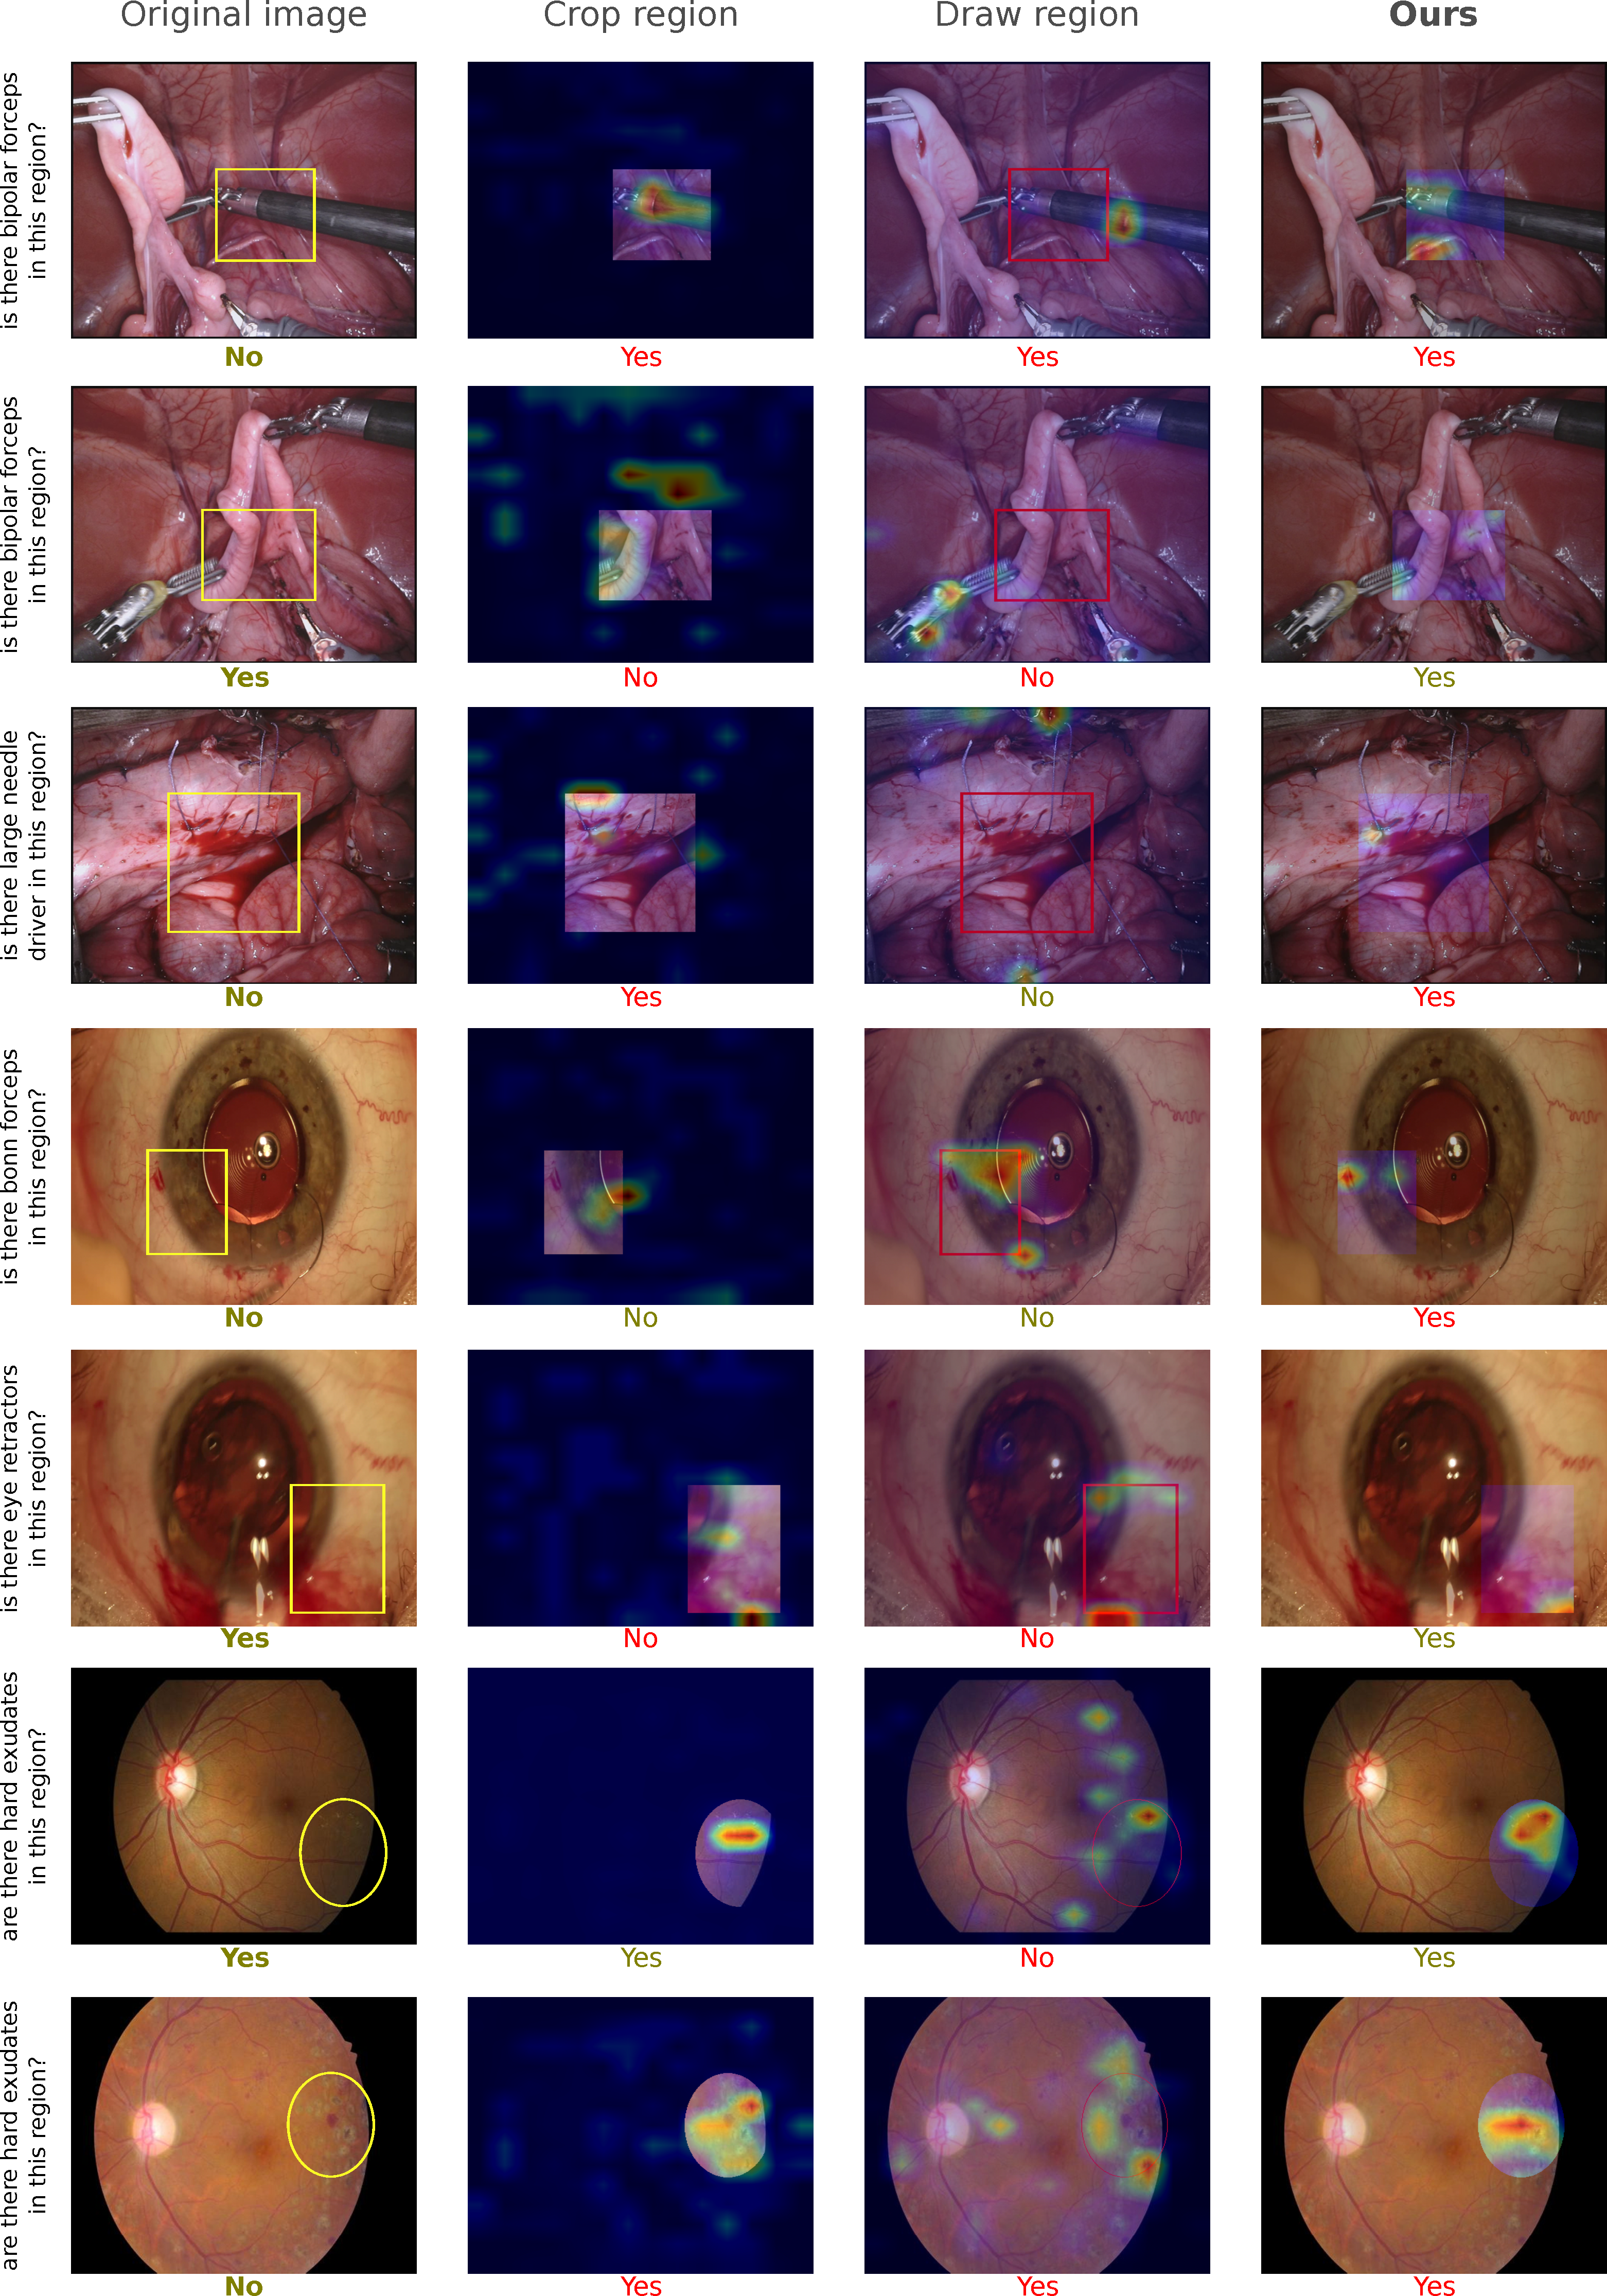
\includegraphics[width=\textwidth]{Figures/Part1_LocVQA/01_locatt/examples_att_supp.pdf}
\caption{Additional qualitative examples from the RIS-VQA (rows 1-3), INSEGCAT-VQA (rows 4-5) and DME-VQA (last two rows) datasets. The first column shows the image, the region, and the ground truth answer. Other columns show the overlaid attention maps and the answers produced by each model. Wrong answers are shown in red.}
\label{fig:examples_supp1}
\end{center}
\end{figure}




\chapter{Targeted Visual Prompting for Medical Visual Question Answering}
\label{appendix:locvqallm}

\begin{table}[!h]
\begin{center}
\begin{tabular}{llp{0.1cm}lp{0.1cm}lp{0.1cm}l}
\toprule
\multicolumn{1}{c}{\multirow{2}{*}{Method}} & \multicolumn{7}{c}{Accuracy (\%)}                                                                                                                                               \\ \cmidrule{2-8} 
\multicolumn{1}{c}{} & \multicolumn{1}{c}{Overall}      && \multicolumn{1}{c}{Grade}        && \multicolumn{1}{c}{Whole}        && \multicolumn{1}{c}{Macula}      \\ \midrule 
No Mask & \multicolumn{1}{c}{60.50} && \multicolumn{1}{c}{81.13} && \multicolumn{1}{c}{76.42} && \multicolumn{1}{c}{85.85}                \\ 
Region in Text & \multicolumn{1}{c}{ 64.75} && \multicolumn{1}{c}{79.25} && \multicolumn{1}{c}{83.96} && \multicolumn{1}{c}{ 82.08}        \\ 
Crop Region  & \multicolumn{1}{c}{86.05} && \multicolumn{1}{c}{80.19} && \multicolumn{1}{c}{83.96} && \multicolumn{1}{c}{84.91}                \\
Draw Region  & \multicolumn{1}{c}{ 86.18} && \multicolumn{1}{c}{79.25} && \multicolumn{1}{c}{83.02} && \multicolumn{1}{c}{83.02}              \\
Context Only  & \multicolumn{1}{c}{ 82.61} && \multicolumn{1}{c}{76.42} && \multicolumn{1}{c}{87.74} && \multicolumn{1}{c}{90.57}              \\
\ours                                          & \multicolumn{1}{c}{89.29} && \multicolumn{1}{c}{79.25} && \multicolumn{1}{c}{83.96} && \multicolumn{1}{c}{84.91}              \\ \bottomrule
\end{tabular}
\end{center}
\caption{Accuracy for the DME-VQA dataset by question type.}
\label{tab:locvqallm_results_dme_appendix}
\end{table}


\begin{figure}[!h]
\begin{center}
\includegraphics[width=\textwidth]{Figures/Part1_LocVQA/02_llm/supplementary_errors_by_location.pdf}
\caption{Error analysis by region location for the four strongest baselines for the RIS-VQA dataset. The maps are obtained by adding binary masks representing the regions for all QA pairs in each category and then normalizing.}
\label{fig:supplementary_errors_by_location}
\end{center}
\end{figure}

\begin{figure}[!h]
\begin{center}
\includegraphics[width=\textwidth]{Figures/Part1_LocVQA/02_llm/examples_supplementary.pdf}
\caption{Additional examples for DME-VQA (rows 1 and 2), RIS-VQA (rows 3 and 4) and Insegcat-VQA (rows 5 and 6).}
\label{fig:examples_supplementary_dme}
\end{center}
\end{figure}	
\chapter{Consistency-preserving Visual Question Answering in Medical Imaging}
\label{appendix:consistency_mainsub}

\begin{figure}[!b]
\begin{center}
\includegraphics[width=\textwidth]{Figures/Part2_Consist/01_mainsub/boxplots.pdf}
\caption{Effect of the variation of the hyperparameters $\lambda$ and $\gamma$, for each metric. The first 5 rows refer to accuracy for all questions (overall), for main questions (main) and for sub-questions (whole, macula and regions). The last two rows correspond to the consistency. In general, a higher value of $\lambda$ leads to a higher consistency, which is the expected behavior. High values of both parameters can produce a decrease in the accuracy of main questions.}
\label{fig:supp_boxplots}
\end{center}
\end{figure}

\begin{figure}[!t]
\begin{center}
\includegraphics[width=\textwidth]{Figures/Part2_Consist/01_mainsub/examples_supplementary_ext.pdf}
\caption{Additional qualitative examples from the DME dataset. Inconsistent answers are highlighted in red. A more consistent behavior is observed in our method in comparison to the baselines (rows 1-2). Even though our method can make mistakes (rows 3-4), it also shows an improvement in the performance on main questions (rows 5-6).}
\label{fig:supp_examples}
\end{center}
\end{figure}	
\chapter{Logical Implications for Visual Question Answering Consistency}
\label{appendix:consistency_logic}

\begin{figure*}[!b]
\centering
\includegraphics[width=0.85\textwidth]{Figures/Part2_Consist/02_logic/examples_ban_supplementary1.pdf}
\caption{Additional qualitative examples from the Introspect dataset using BAN as the backbone. Red siren symbols indicate inconsistent cases. }
\label{fig:examples_introspect1}
\end{figure*}

\begin{figure*}[!t]
\centering
\includegraphics[width=0.85\textwidth]{Figures/Part2_Consist/02_logic/examples_ban_supplementary2.pdf}
\caption{Additional qualitative examples from the Introspect dataset using BAN as the backbone. Red siren symbols indicate inconsistent cases.}
\label{fig:examples_introspect2}
\end{figure*}

\begin{figure*}[!t]
\centering
\includegraphics[width=0.85\textwidth]{Figures/Part2_Consist/02_logic/examples_ban_supplementary3.pdf}
\caption{Additional qualitative examples from the Introspect dataset using BAN as the backbone. Red siren symbols indicate inconsistent cases.}
\label{fig:examples_introspect3}
\end{figure*}

\begin{figure*}[!t]
\centering
\includegraphics[width=0.85\textwidth]{Figures/Part2_Consist/02_logic/examples_ban_supplementary4.pdf}
\caption{Additional qualitative examples from the Introspect dataset using BAN as the backbone. Red siren symbols indicate inconsistent cases.}
\label{fig:examples_introspect4}
\end{figure*}


\begin{figure*}[!t]
\centering
\includegraphics[width=0.85\textwidth]{Figures/Part2_Consist/02_logic/examples_dme_supplementary1.pdf}
\caption{Additional qualitative examples from the DME dataset using MVQA as the backbone. Red siren symbols indicate inconsistent cases. DME is a disease that is staged into grades (0, 1 or 2), which depend on the number of visual pathological features of the retina.}
\label{fig:examples_introspect5}
\end{figure*}


\begin{figure*}[!t]
\centering
\includegraphics[width=0.85\textwidth]{Figures/Part2_Consist/02_logic/examples_dme_supplementary2.pdf}
\caption{Additional qualitative examples from the DME dataset using MVQA as the backbone. Red siren symbols indicate inconsistent cases.}
\label{fig:examples_introspect6}
\end{figure*}	
\@openrighttrue\makeatother

\backmatter
%\cleardoublepage
\phantomsection
\addcontentsline{toc}{chapter}{References}
\printbibliography

% To add bib files, go to head/settings_epfl_template.tex, line 28
%%%%%%%%%%%%%%%%%%%%%%%%%%%%%%%%%%%%%%%%%%%%%%
%%%%% BACK PAGES: Declaration of Originality, CV
%%%%%%%%%%%%%%%%%%%%%%%%%%%%%%%%%%%%%%%%%%%%%%
%----------------------------------------------------------------------------------------
%	BACK PAGES - Declaration of Originality
%----------------------------------------------------------------------------------------

\begin{declaration}
	\addchaptertocentry{\authorshipname} % Add the declaration to the table of contents
	
	\vspace{1cm}
	
	\noindent {\large \bfseries Last name, first name: \authorname \par} \vspace{0.5cm}
	
	\noindent {\large \bfseries Matriculation number: \matriculationnum \par} \vspace{2cm}
	
	{\noindent I  hereby  declare  that  this  thesis represents my  original  work and  that  I  have  used  no  other sources except as noted by citations.\\
		All  data,  tables,  figures  and  text  citations  which  have  been  reproduced  from  any  other source, including the internet, have been explicitly acknowledged as such.\\
		I am aware that in case of non-compliance, the Senate is entitled to withdraw the doctorate degree awarded to me on the basis of the present thesis, in accordance with the “Statut der Universität Bern (Universitätsstatut; UniSt)”, Art. 69, of 7 June 2011.\par} \vspace{1cm}
	
	
	\noindent {Place, Date: \textbf{Bern, March 6, 2024}\par} \vspace{1cm}
	\noindent {Signature:}
    \begin{figure}[h]
    %\begin{right}
    \includegraphics[width=0.3\textwidth]{Figures/signature.png}
    %\end{center}
    \end{figure}
 
\end{declaration}
\include{tail/cv}

%\listoftodos

\end{document}
